%%%%%%%%%%%%%%%%%%%%%%%%%%%%%%%%%%%%%%%%%
% The Legrand Orange Book
% LaTeX Template
% Version 2.4 (26/09/2018)
%
% This template was downloaded from:
% http://www.LaTeXTemplates.com
%
% Original author:
% Mathias Legrand (legrand.mathias@gmail.com) with modifications by:
% Vel (vel@latextemplates.com)
%
% License:
% CC BY-NC-SA 3.0 (http://creativecommons.org/licenses/by-nc-sa/3.0/)
%
% Compiling this template:
% This template uses biber for its bibliography and makeindex for its index.
% When you first open the template, compile it from the command line with the 
% commands below to make sure your LaTeX distribution is configured correctly:
%
% 1) pdflatex main
% 2) makeindex main.idx -s StyleInd.ist
% 3) biber main
% 4) pdflatex main x 2
%
% After this, when you wish to update the bibliography/index use the appropriate
% command above and make sure to compile with pdflatex several times 
% afterwards to propagate your changes to the document.
%
% This template also uses a number of packages which may need to be
% updated to the newest versions for the template to compile. It is strongly
% recommended you update your LaTeX distribution if you have any
% compilation errors.
%
% Important note:
% Chapter heading images should have a 2:1 width:height ratio,
% e.g. 920px width and 460px height.
%
%%%%%%%%%%%%%%%%%%%%%%%%%%%%%%%%%%%%%%%%%

%----------------------------------------------------------------------------------------
%	PACKAGES AND OTHER DOCUMENT CONFIGURATIONS
%----------------------------------------------------------------------------------------

\documentclass[11pt,fleqn]{book} % Default font size and left-justified equations





\usepackage[dvipsnames]{xcolor}






%%%%%%%%%%%%%%%%%%%%%%%%%%%%%%%%%%%%%%%%%
% The Legrand Orange Book
% Structural Definitions File
% Version 2.1 (26/09/2018)
%
% Original author:
% Mathias Legrand (legrand.mathias@gmail.com) with modifications by:
% Vel (vel@latextemplates.com)
% 
% This file was downloaded from:
% http://www.LaTeXTemplates.com
%
% License:
% CC BY-NC-SA 3.0 (http://creativecommons.org/licenses/by-nc-sa/3.0/)
%
%%%%%%%%%%%%%%%%%%%%%%%%%%%%%%%%%%%%%%%%%

%----------------------------------------------------------------------------------------
%	VARIOUS REQUIRED PACKAGES AND CONFIGURATIONS
%----------------------------------------------------------------------------------------

\usepackage{graphicx} % Required for including pictures
\graphicspath{{Pictures/}} % Specifies the directory where pictures are stored

\usepackage{lipsum} % Inserts dummy text

\usepackage{tikz} % Required for drawing custom shapes

\usepackage[english]{babel} % English language/hyphenation

\usepackage[shortlabels]{enumitem}


% \usepackage{enumitem} % Customize lists
\setlist{nolistsep} % Reduce spacing between bullet points and numbered lists

\usepackage{booktabs} % Required for nicer horizontal rules in tables

\usepackage{xcolor} % Required for specifying colors by name
\definecolor{ocre}{RGB}{243,102,25} % Define the orange color used for highlighting throughout the book
\linespread{1.25}
%----------------------------------------------------------------------------------------
%	MARGINS
%----------------------------------------------------------------------------------------

\usepackage{geometry} % Required for adjusting page dimensions and margins

\geometry{
	paper=a4paper, % Paper size, change to letterpaper for US letter size
	top=3cm, % Top margin
	bottom=3cm, % Bottom margin
	left=3cm, % Left margin
	right=3cm, % Right margin
	headheight=14pt, % Header height
	footskip=1.4cm, % Space from the bottom margin to the baseline of the footer
	headsep=10pt, % Space from the top margin to the baseline of the header
	%showframe, % Uncomment to show how the type block is set on the page
}




\usepackage[normalem]{ulem}
\usepackage{amsmath}
\usepackage[english]{babel}
\usepackage{graphicx}
\usepackage{tabulary}
\usepackage{tabularx}
\usepackage{cancel}
\usepackage{pagecolor}
\usepackage{afterpage}
\usepackage{soul}
\usepackage{fixltx2e}
\usepackage[utf8]{inputenc}
\usepackage{siunitx} %degrees for Laboratory
\usepackage{pdflscape} %sidescape figure in Laboratory
\usepackage{float}
\usepackage{afterpage}
\usepackage{xcolor}
\usepackage{framed}
\usepackage{soul}
%\textsubscript{this}
\usepackage{lastpage}
\usepackage[utf8]{inputenc}
\usepackage{ifthen}
\usepackage{amsmath}
\usepackage{fancyhdr}
\usepackage[document]{ragged2e}
% \usepackage[margin=1in,top=1.2in,headheight=57pt,headsep=0.1in]{geometry}
\usepackage{fancyhdr}
\usepackage{caption}
\usepackage{subcaption}
%Chapter 2
\usetikzlibrary{calc}
\usetikzlibrary{arrows}
\usepackage{rotating}%for sidewaysfigure
\usepackage[final]{pdfpages}
\usepackage{gensymb}
\usepackage{tcolorbox}
%\usepackage[dvipsnames]{xcolor}
\usepackage{colortbl}
\usepackage{chemfig}
\usepackage{lscape}
\usepackage{wrapfig}
\usepackage{float}
% FOR CENTERING TEXT IN TABLE
\usepackage{array}
\newcolumntype{C}[1]{>{\centering\arraybackslash}m{#1}}







%----------------------------------------------------------------------------------------
%	FONTS
%----------------------------------------------------------------------------------------

\usepackage{avant} % Use the Avantgarde font for headings
%\usepackage{times} % Use the Times font for headings
\usepackage{mathptmx} % Use the Adobe Times Roman as the default text font together with math symbols from the Sym­bol, Chancery and Com­puter Modern fonts

\usepackage{microtype} % Slightly tweak font spacing for aesthetics
\usepackage[utf8]{inputenc} % Required for including letters with accents
\usepackage[T1]{fontenc} % Use 8-bit encoding that has 256 glyphs

%----------------------------------------------------------------------------------------
%	BIBLIOGRAPHY AND INDEX
%----------------------------------------------------------------------------------------

\usepackage[style=numeric,citestyle=numeric,sorting=nyt,sortcites=true,autopunct=true,babel=hyphen,hyperref=true,abbreviate=false,backref=true,backend=biber]{biblatex}
\addbibresource{bibliography.bib} % BibTeX bibliography file
\defbibheading{bibempty}{}

\usepackage{calc} % For simpler calculation - used for spacing the index letter headings correctly
\usepackage{makeidx} % Required to make an index
\makeindex % Tells LaTeX to create the files required for indexing

%----------------------------------------------------------------------------------------
%	MAIN TABLE OF CONTENTS
%----------------------------------------------------------------------------------------

\usepackage{titletoc} % Required for manipulating the table of contents

\contentsmargin{0cm} % Removes the default margin

% Part text styling (this is mostly taken care of in the PART HEADINGS section of this file)
\titlecontents{part}
	[0cm] % Left indentation
	{\addvspace{5pt}\bfseries} % Spacing and font options for parts
	{}
	{}
	{}

% Chapter text styling
\titlecontents{chapter}
	[1.25cm] % Left indentation
	{\addvspace{12pt}\large\sffamily\bfseries} % Spacing and font options for chapters
	{\color{ocre!60}\contentslabel[\Large\thecontentslabel]{1.25cm}\color{ocre}} % Formatting of numbered sections of this type
	{\color{ocre}} % Formatting of numberless sections of this type
	{\color{ocre!60}\normalsize\;\titlerule*[.5pc]{.}\;\thecontentspage} % Formatting of the filler to the right of the heading and the page number

% Section text styling
\titlecontents{section}
	[1.25cm] % Left indentation
	{\addvspace{3pt}\sffamily\bfseries} % Spacing and font options for sections
	{\contentslabel[\thecontentslabel]{1.25cm}} % Formatting of numbered sections of this type
	{} % Formatting of numberless sections of this type
	{\hfill\color{black}\thecontentspage} % Formatting of the filler to the right of the heading and the page number

% Subsection text styling
\titlecontents{subsection}
	[1.25cm] % Left indentation
	{\addvspace{1pt}\sffamily\small} % Spacing and font options for subsections
	{\contentslabel[\thecontentslabel]{1.25cm}} % Formatting of numbered sections of this type
	{} % Formatting of numberless sections of this type
	{\ \titlerule*[.5pc]{.}\;\thecontentspage} % Formatting of the filler to the right of the heading and the page number

% Figure text styling
\titlecontents{figure}
	[1.25cm] % Left indentation
	{\addvspace{1pt}\sffamily\small} % Spacing and font options for figures
	{\thecontentslabel\hspace*{1em}} % Formatting of numbered sections of this type
	{} % Formatting of numberless sections of this type
	{\ \titlerule*[.5pc]{.}\;\thecontentspage} % Formatting of the filler to the right of the heading and the page number

% Table text styling
\titlecontents{table}
	[1.25cm] % Left indentation
	{\addvspace{1pt}\sffamily\small} % Spacing and font options for tables
	{\thecontentslabel\hspace*{1em}} % Formatting of numbered sections of this type
	{} % Formatting of numberless sections of this type
	{\ \titlerule*[.5pc]{.}\;\thecontentspage} % Formatting of the filler to the right of the heading and the page number

%----------------------------------------------------------------------------------------
%	MINI TABLE OF CONTENTS IN PART HEADS
%----------------------------------------------------------------------------------------

% Chapter text styling
\titlecontents{lchapter}
	[0em] % Left indentation
	{\addvspace{15pt}\large\sffamily\bfseries} % Spacing and font options for chapters
	{\color{ocre}\contentslabel[\Large\thecontentslabel]{1.25cm}\color{ocre}} % Chapter number
	{}  
	{\color{ocre}\normalsize\sffamily\bfseries\;\titlerule*[.5pc]{.}\;\thecontentspage} % Page number

% Section text styling
\titlecontents{lsection}
	[0em] % Left indentation
	{\sffamily\small} % Spacing and font options for sections
	{\contentslabel[\thecontentslabel]{1.25cm}} % Section number
	{}
	{}

% Subsection text styling (note these aren't shown by default, display them by searchings this file for tocdepth and reading the commented text)
\titlecontents{lsubsection}
	[.5em] % Left indentation
	{\sffamily\footnotesize} % Spacing and font options for subsections
	{\contentslabel[\thecontentslabel]{1.25cm}}
	{}
	{}

%----------------------------------------------------------------------------------------
%	HEADERS AND FOOTERS
%----------------------------------------------------------------------------------------

\usepackage{fancyhdr} % Required for header and footer configuration

\pagestyle{fancy} % Enable the custom headers and footers

\renewcommand{\chaptermark}[1]{\markboth{\sffamily\normalsize\bfseries\chaptername\ \thechapter.\ #1}{}} % Styling for the current chapter in the header
\renewcommand{\sectionmark}[1]{\markright{\sffamily\normalsize\thesection\hspace{5pt}#1}{}} % Styling for the current section in the header

\fancyhf{} % Clear default headers and footers
\fancyhead[LE,RO]{\sffamily\normalsize\thepage} % Styling for the page number in the header
\fancyhead[LO]{\rightmark} % Print the nearest section name on the left side of odd pages
\fancyhead[RE]{\leftmark} % Print the current chapter name on the right side of even pages
%\fancyfoot[C]{\thepage} % Uncomment to include a footer

\renewcommand{\headrulewidth}{0.5pt} % Thickness of the rule under the header

\fancypagestyle{plain}{% Style for when a plain pagestyle is specified
	\fancyhead{}\renewcommand{\headrulewidth}{0pt}%
}

% Removes the header from odd empty pages at the end of chapters
\makeatletter
\renewcommand{\cleardoublepage}{
\clearpage\ifodd\c@page\else
\hbox{}
\vspace*{\fill}
\thispagestyle{empty}
\newpage
\fi}

%----------------------------------------------------------------------------------------
%	THEOREM STYLES
%----------------------------------------------------------------------------------------

\usepackage{amsmath,amsfonts,amssymb,amsthm} % For math equations, theorems, symbols, etc

\newcommand{\intoo}[2]{\mathopen{]}#1\,;#2\mathclose{[}}
\newcommand{\ud}{\mathop{\mathrm{{}d}}\mathopen{}}
\newcommand{\intff}[2]{\mathopen{[}#1\,;#2\mathclose{]}}
\renewcommand{\qedsymbol}{$\blacksquare$}
\newtheorem{notation}{Notation}[chapter]

% Boxed/framed environments
\newtheoremstyle{ocrenumbox}% Theorem style name
{0pt}% Space above
{0pt}% Space below
{\normalfont}% Body font
{}% Indent amount
{\small\bf\sffamily\color{ocre}}% Theorem head font
{\;}% Punctuation after theorem head
{0.25em}% Space after theorem head
{\small\sffamily\color{ocre}\thmname{#1}\nobreakspace\thmnumber{\@ifnotempty{#1}{}\@upn{#2}}% Theorem text (e.g. Theorem 2.1)
\thmnote{\nobreakspace\the\thm@notefont\sffamily\bfseries\color{black}---\nobreakspace#3.}} % Optional theorem note

\newtheoremstyle{blacknumex}% Theorem style name
{5pt}% Space above
{5pt}% Space below
{\normalfont}% Body font
{} % Indent amount
{\small\bf\sffamily}% Theorem head font
{\;}% Punctuation after theorem head
{0.25em}% Space after theorem head
{\small\sffamily{\tiny\ensuremath{\blacksquare}}\nobreakspace\thmname{#1}\nobreakspace\thmnumber{\@ifnotempty{#1}{}\@upn{#2}}% Theorem text (e.g. Theorem 2.1)
\thmnote{\nobreakspace\the\thm@notefont\sffamily\bfseries---\nobreakspace#3.}}% Optional theorem note

\newtheoremstyle{blacknumbox} % Theorem style name
{0pt}% Space above
{0pt}% Space below
{\normalfont}% Body font
{}% Indent amount
{\small\bf\sffamily}% Theorem head font
{\;}% Punctuation after theorem head
{0.25em}% Space after theorem head
{\small\sffamily\thmname{#1}\nobreakspace\thmnumber{\@ifnotempty{#1}{}\@upn{#2}}% Theorem text (e.g. Theorem 2.1)
\thmnote{\nobreakspace\the\thm@notefont\sffamily\bfseries---\nobreakspace#3.}}% Optional theorem note

% Non-boxed/non-framed environments
\newtheoremstyle{ocrenum}% Theorem style name
{5pt}% Space above
{5pt}% Space below
{\normalfont}% Body font
{}% Indent amount
{\small\bf\sffamily\color{ocre}}% Theorem head font
{\;}% Punctuation after theorem head
{0.25em}% Space after theorem head
{\small\sffamily\color{ocre}\thmname{#1}\nobreakspace\thmnumber{\@ifnotempty{#1}{}\@upn{#2}}% Theorem text (e.g. Theorem 2.1)
\thmnote{\nobreakspace\the\thm@notefont\sffamily\bfseries\color{black}---\nobreakspace#3.}} % Optional theorem note
\makeatother

% Defines the theorem text style for each type of theorem to one of the three styles above
\newcounter{dummy} 
\numberwithin{dummy}{section}
\theoremstyle{ocrenumbox}
\newtheorem{theoremeT}[dummy]{Theorem}
\newtheorem{problem}{Problem}[chapter]
\newtheorem{exerciseT}{Exercise}[chapter]
\theoremstyle{blacknumex}
\newtheorem{exampleT}{Example}[chapter]
\theoremstyle{blacknumbox}
\newtheorem{vocabulary}{Vocabulary}[chapter]
\newtheorem{definitionT}{Definition}[section]
\newtheorem{corollaryT}[dummy]{Corollary}
\theoremstyle{ocrenum}
\newtheorem{proposition}[dummy]{Proposition}

%----------------------------------------------------------------------------------------
%	DEFINITION OF COLORED BOXES
%----------------------------------------------------------------------------------------

\RequirePackage[framemethod=default]{mdframed} % Required for creating the theorem, definition, exercise and corollary boxes

% Theorem box
\newmdenv[skipabove=7pt,
skipbelow=7pt,
backgroundcolor=black!5,
linecolor=ocre,
innerleftmargin=5pt,
innerrightmargin=5pt,
innertopmargin=5pt,
leftmargin=0cm,
rightmargin=0cm,
innerbottommargin=5pt]{tBox}

% Exercise box	  
\newmdenv[skipabove=7pt,
skipbelow=7pt,
rightline=false,
leftline=true,
topline=false,
bottomline=false,
backgroundcolor=ocre!10,
linecolor=ocre,
innerleftmargin=5pt,
innerrightmargin=5pt,
innertopmargin=5pt,
innerbottommargin=5pt,
leftmargin=0cm,
rightmargin=0cm,
linewidth=4pt]{eBox}	

% Definition box
\newmdenv[skipabove=7pt,
skipbelow=7pt,
rightline=false,
leftline=true,
topline=false,
bottomline=false,
linecolor=ocre,
innerleftmargin=5pt,
innerrightmargin=5pt,
innertopmargin=0pt,
leftmargin=0cm,
rightmargin=0cm,
linewidth=4pt,
innerbottommargin=0pt]{dBox}	

% Corollary box
\newmdenv[skipabove=7pt,
skipbelow=7pt,
rightline=false,
leftline=true,
topline=false,
bottomline=false,
linecolor=gray,
backgroundcolor=black!5,
innerleftmargin=5pt,
innerrightmargin=5pt,
innertopmargin=5pt,
leftmargin=0cm,
rightmargin=0cm,
linewidth=4pt,
innerbottommargin=5pt]{cBox}

% Creates an environment for each type of theorem and assigns it a theorem text style from the "Theorem Styles" section above and a colored box from above
\newenvironment{theorem}{\begin{tBox}\begin{theoremeT}}{\end{theoremeT}\end{tBox}}
\newenvironment{exercise}{\begin{eBox}\begin{exerciseT}}{\hfill{\color{ocre}\tiny\ensuremath{\blacksquare}}\end{exerciseT}\end{eBox}}				  
\newenvironment{definition}{\begin{dBox}\begin{definitionT}}{\end{definitionT}\end{dBox}}	
\newenvironment{example}{\begin{exampleT}}{\hfill{\tiny\ensuremath{\blacksquare}}\end{exampleT}}		
\newenvironment{corollary}{\begin{cBox}\begin{corollaryT}}{\end{corollaryT}\end{cBox}}	

%----------------------------------------------------------------------------------------
%	REMARK ENVIRONMENT
%----------------------------------------------------------------------------------------

\newenvironment{remark}{\par\vspace{10pt}\small % Vertical white space above the remark and smaller font size
\begin{list}{}{
\leftmargin=35pt % Indentation on the left
\rightmargin=25pt}\item\ignorespaces % Indentation on the right
\makebox[-2.5pt]{\begin{tikzpicture}[overlay]
\node[draw=ocre!60,line width=1pt,circle,fill=ocre!25,font=\sffamily\bfseries,inner sep=2pt,outer sep=0pt] at (-15pt,0pt){\textcolor{ocre}{R}};\end{tikzpicture}} % Orange R in a circle
\advance\baselineskip -1pt}{\end{list}\vskip5pt} % Tighter line spacing and white space after remark

%----------------------------------------------------------------------------------------
%	SECTION NUMBERING IN THE MARGIN
%----------------------------------------------------------------------------------------

\makeatletter
\renewcommand{\@seccntformat}[1]{\llap{\textcolor{ocre}{\csname the#1\endcsname}\hspace{1em}}}                    
\renewcommand{\section}{\@startsection{section}{1}{\z@}
{-4ex \@plus -1ex \@minus -.4ex}
{1ex \@plus.2ex }
{\normalfont\large\sffamily\bfseries}}
\renewcommand{\subsection}{\@startsection {subsection}{2}{\z@}
{-3ex \@plus -0.1ex \@minus -.4ex}
{0.5ex \@plus.2ex }
{\normalfont\sffamily\bfseries}}
\renewcommand{\subsubsection}{\@startsection {subsubsection}{3}{\z@}
{-2ex \@plus -0.1ex \@minus -.2ex}
{.2ex \@plus.2ex }
{\normalfont\small\sffamily\bfseries}}                        
\renewcommand\paragraph{\@startsection{paragraph}{4}{\z@}
{-2ex \@plus-.2ex \@minus .2ex}
{.1ex}
{\normalfont\small\sffamily\bfseries}}

%----------------------------------------------------------------------------------------
%	PART HEADINGS
%----------------------------------------------------------------------------------------

% Numbered part in the table of contents
\newcommand{\@mypartnumtocformat}[2]{%
	\setlength\fboxsep{0pt}%
	\noindent\colorbox{ocre!20}{\strut\parbox[c][.7cm]{\ecart}{\color{ocre!70}\Large\sffamily\bfseries\centering#1}}\hskip\esp\colorbox{ocre!40}{\strut\parbox[c][.7cm]{\linewidth-\ecart-\esp}{\Large\sffamily\centering#2}}%
}

% Unnumbered part in the table of contents
\newcommand{\@myparttocformat}[1]{%
	\setlength\fboxsep{0pt}%
	\noindent\colorbox{ocre!40}{\strut\parbox[c][.7cm]{\linewidth}{\Large\sffamily\centering#1}}%
}

\newlength\esp
\setlength\esp{4pt}
\newlength\ecart
\setlength\ecart{1.2cm-\esp}
\newcommand{\thepartimage}{}%
\newcommand{\partimage}[1]{\renewcommand{\thepartimage}{#1}}%
\def\@part[#1]#2{%
\ifnum \c@secnumdepth >-2\relax%
\refstepcounter{part}%
\addcontentsline{toc}{part}{\texorpdfstring{\protect\@mypartnumtocformat{\thepart}{#1}}{\partname~\thepart\ ---\ #1}}
\else%
\addcontentsline{toc}{part}{\texorpdfstring{\protect\@myparttocformat{#1}}{#1}}%
\fi%
\startcontents%
\markboth{}{}%
{\thispagestyle{empty}%
\begin{tikzpicture}[remember picture,overlay]%
\node at (current page.north west){\begin{tikzpicture}[remember picture,overlay]%	
\fill[ocre!20](0cm,0cm) rectangle (\paperwidth,-\paperheight);
\node[anchor=north] at (4cm,-3.25cm){\color{ocre!40}\fontsize{220}{100}\sffamily\bfseries\thepart}; 
\node[anchor=south east] at (\paperwidth-1cm,-\paperheight+1cm){\parbox[t][][t]{8.5cm}{
\printcontents{l}{0}{\setcounter{tocdepth}{1}}% The depth to which the Part mini table of contents displays headings; 0 for chapters only, 1 for chapters and sections and 2 for chapters, sections and subsections
}};
\node[anchor=north east] at (\paperwidth-1.5cm,-3.25cm){\parbox[t][][t]{15cm}{\strut\raggedleft\color{Black}\fontsize{30}{30}\sffamily\bfseries#2}};
\end{tikzpicture}};
\end{tikzpicture}}%
\@endpart}
\def\@spart#1{%
\startcontents%
\phantomsection
{\thispagestyle{empty}%
\begin{tikzpicture}[remember picture,overlay]%
\node at (current page.north west){\begin{tikzpicture}[remember picture,overlay]%	
\fill[ocre!20](0cm,0cm) rectangle (\paperwidth,-\paperheight);
\node[anchor=north east] at (\paperwidth-1.5cm,-3.25cm){\parbox[t][][t]{15cm}{\strut\raggedleft\color{white}\fontsize{30}{30}\sffamily\bfseries#1}};
\end{tikzpicture}};
\end{tikzpicture}}
\addcontentsline{toc}{part}{\texorpdfstring{%
\setlength\fboxsep{0pt}%
\noindent\protect\colorbox{ocre!40}{\strut\protect\parbox[c][.7cm]{\linewidth}{\Large\sffamily\protect\centering #1\quad\mbox{}}}}{#1}}%
\@endpart}
\def\@endpart{\vfil\newpage
\if@twoside
\if@openright
\null
\thispagestyle{empty}%
\newpage
\fi
\fi
\if@tempswa
\twocolumn
\fi}

%----------------------------------------------------------------------------------------
%	CHAPTER HEADINGS
%----------------------------------------------------------------------------------------

% A switch to conditionally include a picture, implemented by Christian Hupfer
\newif\ifusechapterimage
\usechapterimagetrue
\newcommand{\thechapterimage}{}%
\newcommand{\chapterimage}[1]{\ifusechapterimage\renewcommand{\thechapterimage}{#1}\fi}%
\newcommand{\autodot}{.}
\def\@makechapterhead#1{%
{\parindent \z@ \raggedright \normalfont
\ifnum \c@secnumdepth >\m@ne
\if@mainmatter
\begin{tikzpicture}[remember picture,overlay]
\node at (current page.north west)
{\begin{tikzpicture}[remember picture,overlay]
\node[anchor=north west,inner sep=0pt] at (0,0) {\ifusechapterimage\includegraphics[width=\paperwidth]{\thechapterimage}\fi};
\draw[anchor=west] (\Gm@lmargin,-9cm) node [line width=2pt,rounded corners=15pt,draw=ocre,fill=white,fill opacity=0.5,inner sep=15pt]{\strut\makebox[22cm]{}};
\draw[anchor=west] (\Gm@lmargin+.3cm,-9cm) node {\huge\sffamily\bfseries\color{black}\thechapter\autodot~#1\strut};
\end{tikzpicture}};
\end{tikzpicture}
\else
\begin{tikzpicture}[remember picture,overlay]
\node at (current page.north west)
{\begin{tikzpicture}[remember picture,overlay]
\node[anchor=north west,inner sep=0pt] at (0,0) {\ifusechapterimage\includegraphics[width=\paperwidth]{\thechapterimage}\fi};
\draw[anchor=west] (\Gm@lmargin,-9cm) node [line width=2pt,rounded corners=15pt,draw=ocre,fill=white,fill opacity=0.5,inner sep=15pt]{\strut\makebox[22cm]{}};
\draw[anchor=west] (\Gm@lmargin+.3cm,-9cm) node {\huge\sffamily\bfseries\color{black}#1\strut};
\end{tikzpicture}};
\end{tikzpicture}
\fi\fi\par\vspace*{270\p@}}}

%-------------------------------------------

\def\@makeschapterhead#1{%
\begin{tikzpicture}[remember picture,overlay]
\node at (current page.north west)
{\begin{tikzpicture}[remember picture,overlay]
\node[anchor=north west,inner sep=0pt] at (0,0) {\ifusechapterimage\includegraphics[width=\paperwidth]{\thechapterimage}\fi};
\draw[anchor=west] (\Gm@lmargin,-9cm) node [line width=2pt,rounded corners=15pt,draw=ocre,fill=white,fill opacity=0.5,inner sep=15pt]{\strut\makebox[22cm]{}};
\draw[anchor=west] (\Gm@lmargin+.3cm,-9cm) node {\huge\sffamily\bfseries\color{black}#1\strut};
\end{tikzpicture}};
\end{tikzpicture}
\par\vspace*{270\p@}}
\makeatother

%----------------------------------------------------------------------------------------
%	LINKS
%----------------------------------------------------------------------------------------

\usepackage{hyperref}
\hypersetup{hidelinks,backref=true,pagebackref=true,hyperindex=true,colorlinks=false,breaklinks=true,urlcolor=ocre,bookmarks=true,bookmarksopen=false}

\usepackage{bookmark}
\bookmarksetup{
open,
numbered,
addtohook={%
\ifnum\bookmarkget{level}=0 % chapter
\bookmarksetup{bold}%
\fi
\ifnum\bookmarkget{level}=-1 % part
\bookmarksetup{color=ocre,bold}%
\fi
}
}
 % Insert the commands.tex file which contains the majority of the structure behind the template

%\hypersetup{pdftitle={Title},pdfauthor={Author}} % Uncomment and fill out to include PDF metadata for the author and title of the book

%----------------------------------------------------------------------------------------

\begin{document}

%----------------------------------------------------------------------------------------
%	TITLE PAGE
%----------------------------------------------------------------------------------------

\begingroup
\thispagestyle{empty} % Suppress headers and footers on the title page
%\begin{center}
%
\includegraphics[scale=0.6]{Blank.png}\\
%
\includegraphics[scale=0.6]{SCC_Logo_Primary.png}
%\end{center}
\newpagecolor{BurntOrange}\afterpage{\restorepagecolor}
\begin{tikzpicture}[remember picture,overlay]
%\node[inner sep=0pt] (background) at (current page.center) {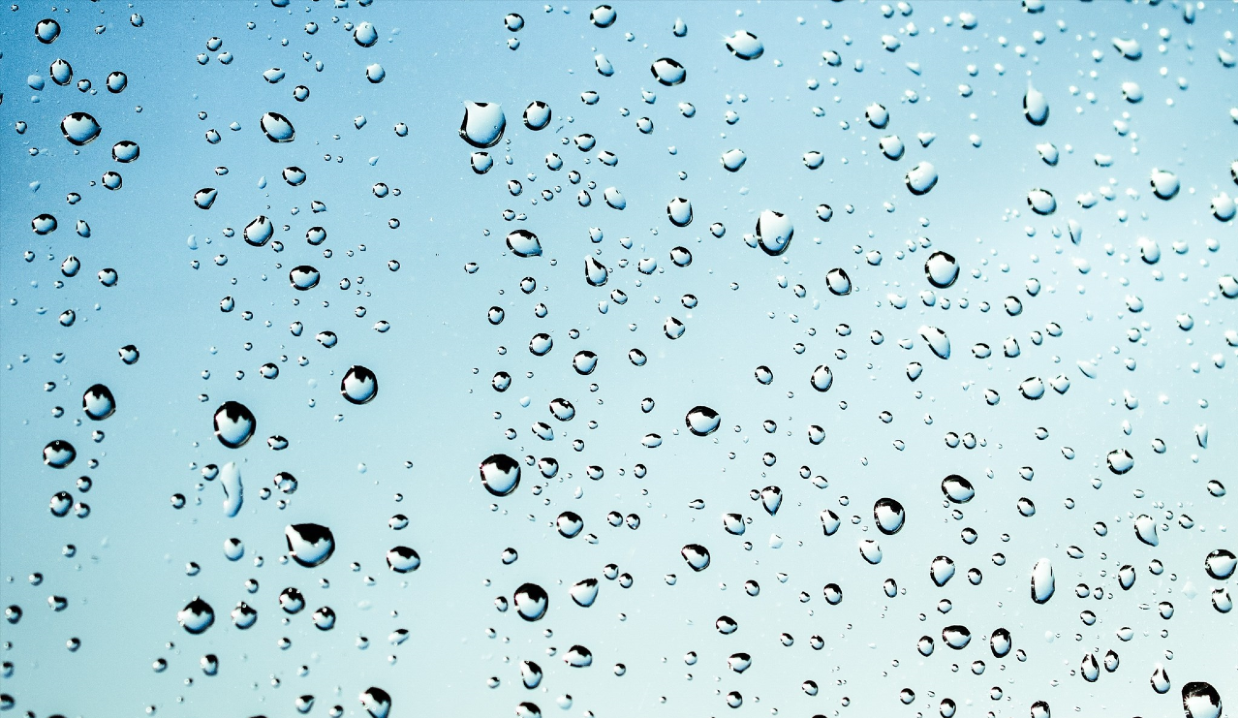
\includegraphics[width=\paperwidth]{Water3.png}};

\node[inner sep=0pt] (background) at (current page.center) {\includegraphics[width=\paperwidth]{WaterBackground1.png}};


\draw (current page.center)node [fill=blue!1!white!10,fill opacity=.3,text opacity=1,inner sep=2cm] { \Huge\centering\bfseries\sffamily\parbox[c][][t]{\paperwidth}{\centering \textcolor{Bittersweet}{WATR 082 - Fall 2021} \\\textcolor{BurntOrange}{Advanced Wastewater Treatment}\\[15pt] % Book title
% {\Large A Profound Subtitle}\\[20pt] % Subtitle
{\large Shabbir Basrai}}}; % Author name
\end{tikzpicture}
\begin{center}

\includegraphics[scale=0.5]{SCC_Logo_Primary.png}
\end{center}
\vfill
\endgroup

%----------------------------------------------------------------------------------------
%	COPYRIGHT PAGE
%----------------------------------------------------------------------------------------

\newpage
~\vfill
\thispagestyle{empty}

\noindent Copyright \copyright\ 2021 Shabbir Basrai\\ % Copyright notice
%
%\noindent \textsc{Published by Publisher}\\ % Publisher
%
%\noindent \textsc{book-website.com}\\ % URL
%
%\noindent Licensed under the Creative Commons Attribution-NonCommercial 3.0 Unported License (the ``License''). You may not use this file except in compliance with the License. You may obtain a copy of the License at \url{http://creativecommons.org/licenses/by-nc/3.0}. Unless required by applicable law or agreed to in writing, software distributed under the License is distributed on an \textsc{``as is'' basis, without warranties or conditions of any kind}, either express or implied. See the License for the specific language governing permissions and limitations under the License.\\ % License information, replace this with your own license (if any)

\noindent \textit{Revision Date: June 2021} % Printing/edition date

%----------------------------------------------------------------------------------------
%	TABLE OF CONTENTS
%----------------------------------------------------------------------------------------

%\usechapterimagefalse % If you don't want to include a chapter image, use this to toggle images off - it can be enabled later with \usechapterimagetrue

\chapterimage{WastewaterTreatmentPlantAerialBandW.jpg} % Table of contents heading image

\pagestyle{empty} % Disable headers and footers for the following pages

\tableofcontents % Print the table of contents itself
\listoffigures
\listoftables
\cleardoublepage % Forces the first chapter to start on an odd page so it's on the right side of the book

\pagestyle{fancy} % Enable headers and footers again

%----------------------------------------------------------------------------------------
%	PART
%----------------------------------------------------------------------------------------



%----------------------------------------------------------------------------------------
%	CHAPTER 1
%----------------------------------------------------------------------------------------

% \chapterimage{chapter_head_2.pdf} % Chapter heading image

% \chapter{Text Chapter}

% \section{Paragraphs of Text}\index{Paragraphs of Text}



% \lipsum[1-7] % Dummy text
% 
%------------------------------------------------

%\section{Citation}\index{Citation}
%
%This statement requires citation \cite{article_key}; this one is more specific \cite[162]{book_key}.

%------------------------------------------------

%\section{Lists}\index{Lists}
%
%Lists are useful to present information in a concise and/or ordered way\footnote{Footnote example...}.
%
%\subsection{Numbered List}\index{Lists!Numbered List}
%
%\begin{enumerate}
%\item The first item
%\item The second item
%\item The third item
%\end{enumerate}
%
%\subsection{Bullet Points}\index{Lists!Bullet Points}
%
%\begin{itemize}
%\item The first item
%\item The second item
%\item The third item
%\end{itemize}
%
%\subsection{Descriptions and Definitions}\index{Lists!Descriptions and Definitions}
%
%\begin{description}
%\item[Name] Description
%\item[Word] Definition
%\item[Comment] Elaboration
%\end{description}


%----------------------------------------------------------------------------------------
%	PART 2
%----------------------------------------------------------------------------------------


%----------------------------------------------------------------------------------------
%	CHAPTER 1
%----------------------------------------------------------------------------------------

%\chapter{Wastewater Math}

\part{Module 1}
\chapterimage{Water1.png} % Chapter heading image

\chapter{Basics of Wastewater Treatment}

\section{Why Treat Wastewater}\index{Why Treat Wastewater}
\begin{itemize}
\item Wastewater is used water from home and industries\\
\item Wastewater must be treated prior to returning it back into the environment - typically into the receiving waters which include lakes, rivers and ocean.


\item Wastewater treatment removes:
\begin{itemize}
\item organic matter
\item inorganic  pollutants including plant nutrients - nitrogen and phosphorous\\
\item pathogenic (disease causing) organisms\\
\end{itemize}

\item Wastewater treatment protects:
\begin{itemize}
\item The environment
\item Human health
\end{itemize}

\item In the receiving waters, inadequately treated wastewater discharge depletes dissolved oxygen levels - \hl{eutrophication}, potentially destructing its normal aquatic life including fish.  Wastewater discharge promotes eutrophication due to:

\begin{itemize}
\item Nutrients such as nitrogen and phosphorous present in wastewater effluent promotes growth of plant and algal matter.  Dissolved oxygen is consumed as a part of the normal decay of this plant and algal matter.  
\item The consumption of organic material present in wastewater discharge by aerobic bacteria also results in oxygen depletion in the receiving waters.  


\end{itemize}
\end{itemize}

\section{Wastewater Treatment Regulations}\index{Wastewater Treatment Regulations}
% \begin{snugshade*}
% \item \noindent\textsc{Wastewater Treatment Regulations}
% \end{snugshade*}

\begin{itemize}
\item The \hl{National Pollutant Discharge Elimination System (NPDES) permit program} was created in 1972 by the Clean Water Act (CWA)
\item Applies to sources that discharge pollutants to waters of the United States.
\item Requires all facilities discharging “pollutants” into any body of water in the USA to obtain and comply with a \hl{NPDES permit}
\item NPDES permit \hl{establishes} \textul{discharge limits}, \textul{monitoring} and \textul{reporting} \hl{requirements}\\
\item The NPDES permitting and enforcement responsibilities have been delegated by the EPA to the State of California for implementation through the \hl{State Water Resources Control Board(SWRCB)} and the \textul{nine} \hl{Regional Water Quality Control Boards (Regional Water Boards)}.
\item In California, NPDES permits are also referred to as waste discharge requirements (WDRs) that regulate discharges to waters of the United States.
\end{itemize}


\section{Wastewater Process Overview}\index{Wastewater Process Overview}
Wastewater treatment involves the following elements:
\subsection{Generation}\index{Generation}
Wastewater originates from domestic, industrial, commercial or agricultural activities. The characteristics of wastewater vary depending on the source. Types of wastewater include: 
\begin{itemize}
\item \hl{Domestic Sewage:}  wastewater derived principally from dwellings, business buildings, institutions, and \\
\item \hl{Industrial Sewage:}  liquid waste from industrial processes\\
\end{itemize}
Typical per person generation of wastewater in the USA is about 70-100 gallons per day

\subsection{Collections}\index{Collections}

\begin{itemize}
\item Wastewater is collected from its point of origin - home, businesses, industries etc. and conveyed via sewer lines to a centralized wastewater treatment facility.  
\item When the rainwater drainage is made part of the sewer system, the system is termed as \hl{Combined System}.  
\item The system where the sewage is conveyed separately from the stormwater flows is termed as \hl{Separated System}.  
\item In the Separated System, the Sanitary Sewers convey the wastewater and the Stormwater Sewer conveys the storm water flows.  
\item For the Combined System, rainstorms pose the threat of overwhelming the sewers and the treatment plant
\end{itemize}


%\begin{figure} 
%
%
%	  	\begin{subfigure}[b]{0.4\linewidth}
%		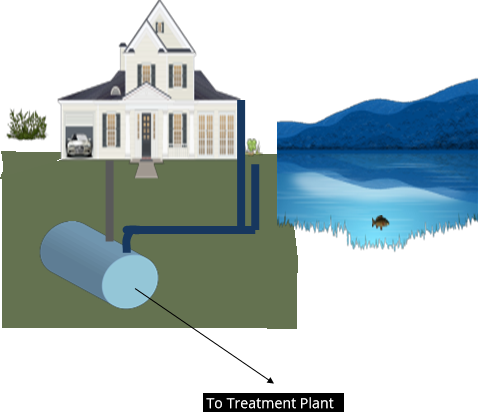
\includegraphics[scale=0.25]{CombinedSystem1} \hspace{0.35cm}
%		\caption{Combined system}
%		\end{subfigure}
%	
%	  	\begin{subfigure}[b]{0.4\linewidth} 
%		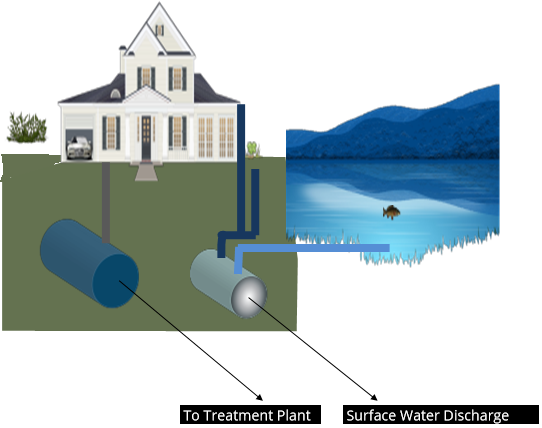
\includegraphics[scale=0.25]{SeperatedSystem1}
%		\caption{Separated systems}
%		\end{subfigure}
%
%
%	\caption{Collections system types}
%
%\end{figure}


	\begin{figure}[h!]
	\centering
  \begin{subfigure}[b]{0.47\linewidth}
  
 \begin{center} 
    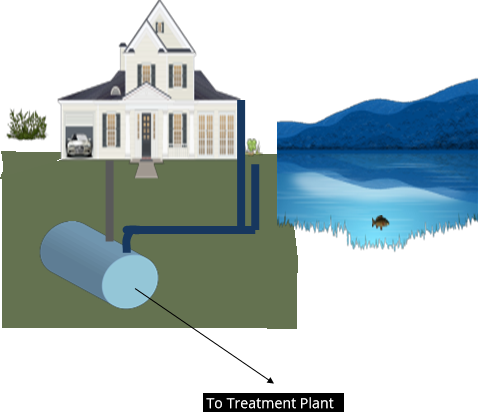
\includegraphics[width=\linewidth]{CombinedSystem1}
    \caption{Combined system}
    \end{center} 
  \end{subfigure}
    \begin{subfigure}[b]{0.50\linewidth}
  \begin{center} 
    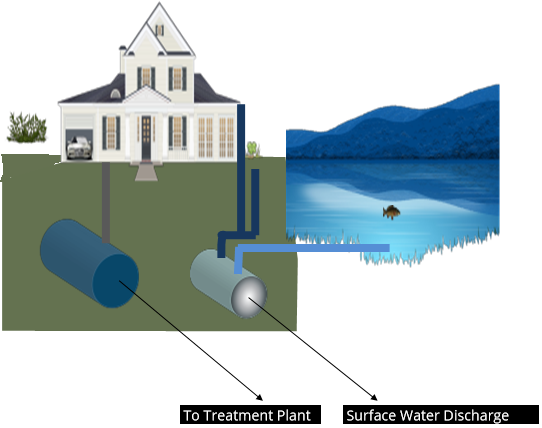
\includegraphics[width=\linewidth]{SeperatedSystem1}
    \caption{Separated systems}
    \end{center} 
  \end{subfigure}
  

  
  \caption{Collections system types}

  \end{figure}



\subsection{Treatment}\index{Treatment}

\begin{itemize}
\item Wastewater treatment includes processes  used for treating the liquid stream and also processes for the treatment of solids which are separated and/or generated during the liquid stream process.
\item The liquid stream wastewater treatment processes involve physical, chemical or biological processes or combinations of these processes depending on the required outflow standards. 
\item Liquid stream is typically treated in a series of steps with increasing level of treatment:
\begin{enumerate}
\item \hl{Preliminary}:  
			
			
		\begin{itemize}
		\item The objective of preliminary treatment is to remove coarse solids and other large materials often found in raw wastewater
		\item Removal of these materials is necessary to enhance the operation and maintenance of subsequent treatment units\\
		\item Preliminary treatment operations typically include a combination of the following processes:
			\begin{itemize}
			\item Screening
			\item Grinding or shredding
			\item Flow measurement
			\item Grit removal
			\item Pre-aeration
			\item Flow equalization
			\end{itemize}
		\end{itemize}
\item \hl{Primary}:
		\begin{itemize}
		\item   The primary process is also a physical process where the separable wastewater solids - solids that float and 			solids that can settle, are removed.
		\item Primary treatment is after preliminary treatment and before secondary treatment
		\item Its two main objectives are: 
			\begin{itemize}
			\item Remove settleable solids
			\item Remove floatable solids
			\end{itemize}
		\item This is a physical process which relies on the physical properties - how heavy or light the suspended solids 				particles are to effect its separation
		\item Provides quiescent conditions for the influent wastewater for the heavier solids to settle and the lighter 				solids to float
		\item Removes settleable solids and floatables
		\item Settled solids are removed as sludge from the bottom of the clarifier
		\item Floatable solids including oil and grease are also removed, as scum from the surface
		\item The shape of the primary clarifier is either rectangular or circular
		\item Effective solids removal in the primary clarifiers will reduce the loading on the expensive secondary treatment 			process.
		\item The amount of solids removed during primary treatment may be enhanced by chemical addition - ferric or ferrous 			chloride as a coagulant and anionic polymer as the flocculant.  This is called Chemically Enhanced Primary Treatment 			(CEPT).
		\end{itemize}
\item \hl{Secondary}:

		\begin{itemize}
		\item While preliminary and primary treatment processes are designed primarily to remove solids from wastewater, 				secondary treatment is for the removal of organics
		\item Secondary treatment is a biological treatment process where microorganisms consume the organic matter present in 			the wastewater.
		\item Secondary treatment involves:
			\begin{itemize}
			\item biological conversion of the dissolved and suspended organics in wastewater into biomass, and
			\item physical settling (separation) process where the solids including the biomass formed during secondary 					treatment is separated and removed from the treated wastewater.
			\end{itemize}
		\item Secondary treatment process incorporates one of the following three approaches:
			\begin{enumerate}
			\item \textbf{Fixed film system}
				\begin{itemize}
				\item Here the microorganisms responsible for the treatment, grow on substrates such
				as rocks, sand or plastic.
				\item When the wastewater is spread over the substrate, the microorganisms up-take the organics present in 						the wastewater
				\item Example of this secondary treatment process include trickling filters and rotating biological 							contactors
				\end{itemize}
			\item \textbf{Suspended Growth System}
				\begin{itemize}
				\item In this type of secondary treatment, the microbes are suspended in the
				wastewater flow being treated. 
				\item Air or oxygen is supplied to maintain an aerobic environment and to keep the microorganisms in 							suspension. 
				\item Example of this secondary treatment approach include the activated sludge treatment process 
				\end{itemize}
			\item \textbf{Pond System}
				\begin{itemize}
				\item Similar to the suspended growth, stabilization ponds are large man made bodies of water which treat 						wastewater using mainly natural processes including sunlight, algae and microorganisms.
				\end{itemize}
			\end{enumerate}
		\end{itemize}


\item \hl{Tertiary or Advanced Treatment:}
	\begin{itemize}
	\item  The tertiary/advanced treatment processes improve the quality of treated water beyond the secondary treatment level. 
	\item  This process may include nutrient removal and disinfection.
	\end{itemize}
	\begin{figure}[h!]
	\centering
\begin{center}
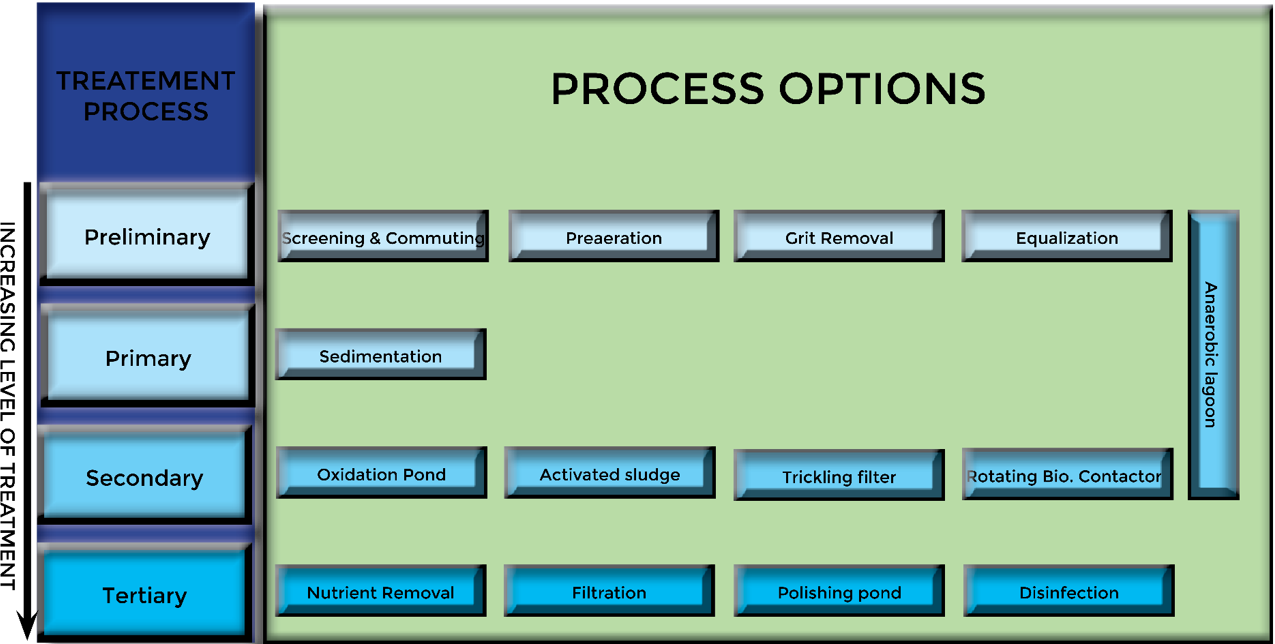
\includegraphics[scale=0.48]{Treatment}
\caption{Process options}
\end{center}
\end{figure}
\end{enumerate}
\vspace{0.5cm}
\item Solids treatment processes are primarily geared to ensure that the solids generated meet the federal regulatory requirements established for wastewater generated solids, at the lowest cost and environmental impact.
\newpage
\textbf{A typical layout/process sequencing in a wastewater treatment plant is shown below:}

	\begin{figure}[h!]
	\centering
\begin{center}
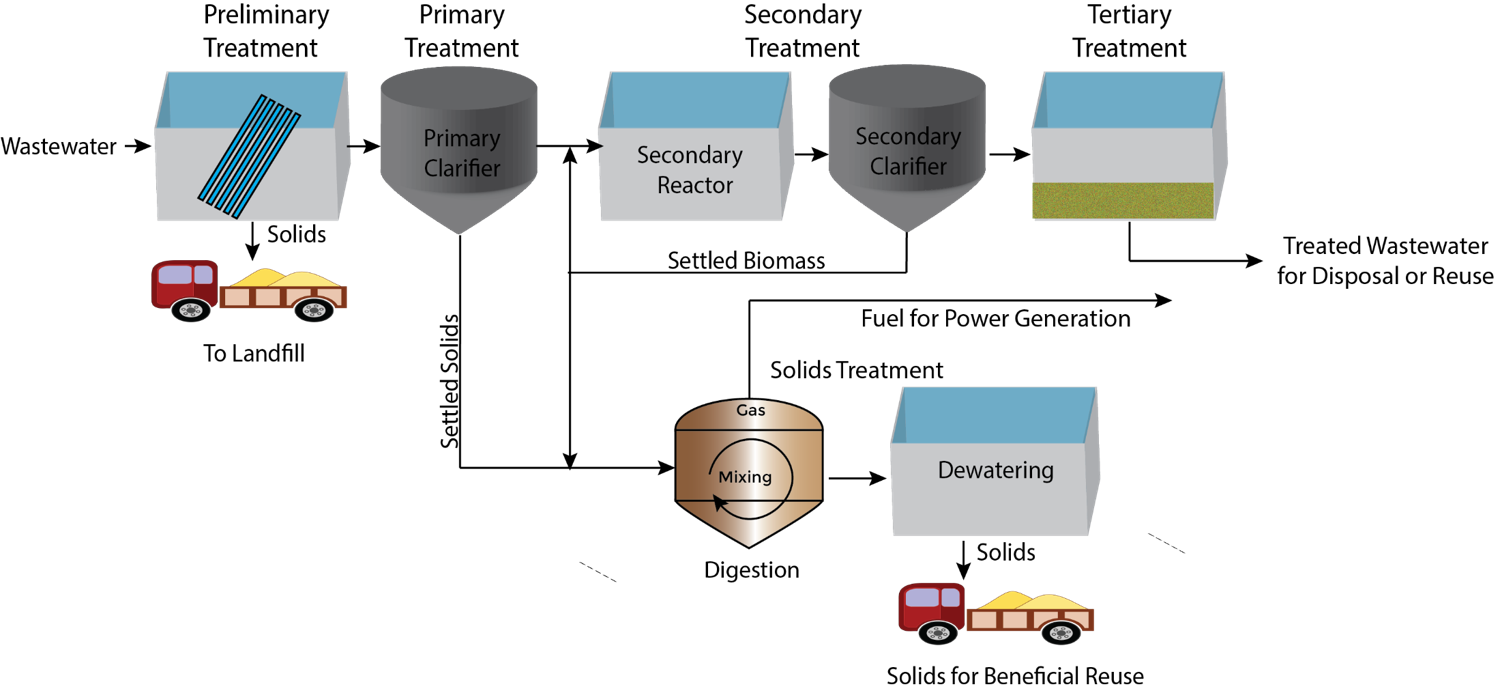
\includegraphics[scale=0.6]{TreatmentFlow}
\end{center}
\caption{Typical wastewater treatment process sequencing}
\end{figure}
\end{itemize}
Individual wastewater treatment processes involve different process options or sequences which are illustrated in Figure 1.3 below:


As the treatment process becomes more advanced along with the increasing awareness of the resources involved in the treatment, there is a move underway to transform Wastewater Treatment Plants (WWTF) to Renewable Resource Recovery Facilities (RRRF) or Water Resource Recovery Facilities (WRRF) - one which produces clean water, recovers energy and generates nutrients.

\subsection{Disposal or Reuse}\index{Disposal or Reuse}

\begin{itemize}
\item Wastewater treatment processes can be designed to \hl{dispose} the treated water where the water is reintroduced to the environment or for \hl{reuse} where the treated water is \hl{reclaimed} or \hl{recycled} - for various purposes including irrigation, industrial use or for potable use.
\item Water disposal methods include:\\
\begin{itemize}
\item \hl{Surface water discharge}
\item \hl{Subsurface discharge}
\end{itemize}
\item Water reuse methods include:\\
\begin{itemize}
\item Potable water reuse
\begin{itemize}
\item \hl{Indirect potable reuse:}  Here the treated water is blended with groundwater or surface water and then reclaimed and treated further 
for drinking (potable) water use
\item \hl{Direct potable reuse:}  Here the treated wastewater is subjected to advanced treatment and introduced directly into a municipal water supply system
\end{itemize}
\item Water reclamation for irrigation or industrial use\\
\item Land application for beneficial use\\
\end{itemize}
\item Solids generated from the wastewater treatment process may be removed and disposed to a landfill or subject to further treatment which may allow for energy recovery - from the organic solids and for beneficial reuse due to its plant nutrient content.\\
\end{itemize}










\chapterimage{MathCover.png} % Chapter heading image

\chapter{Wastewater Math Review}\index{Wastewater Math Review}

\section{Unit Conversions}\index{Unit Conversions}


% \begin{enumerate}
% \definecolor{shadecolor}{RGB}{200, 200, 240}
% \begin{snugshade*}
%\section{Units and Unit Conversion}\index{Units and Unit Conversion}
% 	\item \noindent\textsc{Units and Unit Conversion}
% \end{snugshade*}

For converting one measurement unit to another.

Step 1:  \texthl{Make sure the original unit is for the same measurement as the converted (desired) unit.}  So if the original unit is for area, say in ft$^2$ the converted unit should be another area unit such as in$^2$ or acre but it cannot be gallons as gallon is a unit of volume.

Step 2: Write down the conversion formula as:

$Quantity \enspace in \enspace converted \enspace unit = Quantity \enspace (\cancel{Original \enspace Unit}) *   Conversion  \enspace Factor \enspace  \dfrac{Conversion \enspace unit}{\cancel{Original \enspace unit}}$


\begin{table}[h!]

\begin{center}
    \begin{tabular}{ | p{4cm} |p{8cm}|}
    \hline
    
    
Length  & inches, ft, miles\\
\hline 
Area  & ft$^2$, acres \\
\hline 
Volume & ft$^3$, gallons, acres-ft.\\
\hline 
Density & weight per volume, lbs/ft$^3$, lbs/gallon\\
\hline 
Flow & ft$^3$/min, MGD, acres-ft/day\\
\hline 

	

    \end{tabular}
 \caption{Common units in wastewater calculations}	
    \end{center}

    \end{table}

%Powers of Ten
%
%\begin{center}
%    
%   
%    \begin{tabular}{ | c | p{4cm} | c |p{8cm}|}
%    \hline
%
%%\hline
%%\multicolumn{4}{|c|}{\textbf{ESSAYS}} \\
%%\hline
%%\thead{A Head} & \thead{A Second \\ Head} & \thead{A Third \\ Head} \\
%%\hline%
%
%$10^{12}$ & 1,000,000,000,000 & Tera & Like in tera byte drive - trillion\\
%\hline 
%$10^{9}$ & 1,000,000,000 & Giga & Like in giga byte data - billion\\
%\hline
%$10^{6}$ & 1,000,000 & Mega & Like in mega bytes or megawatts - million\\
%\hline 
%$10^{3}$ & 1,000 & Kilo & Like in kilogram \\
%\hline 
%$10^{0}$ & 1 &  & \\
%\hline 
%$10^{-3}$ & 0.001 & milli & Like in millimeter - thousandth of a meter\\
%\hline 
%$10^{-6}$ & 0.000001 & micro & Like in microgram - millionth of a gram \\
%\hline 
%$10^{-9}$ & 0.000000001 & nano & Like in nanometer - billionth of a meter\\
%\hline 
%
%
%    \end{tabular}
%    
%    \end{center}





\subsection{Example Problems}\index{Example Problems}
\begin{enumerate}
\item Convert 1000 $ft^3$ to cu. yards\\

$1000 \cancel{ft^3}*\dfrac{cu.yards}{27\cancel{ft^3}} = 37 cu.yards$
\vspace{6pt}
\item Convert 10 gallons/min to $ft^3$/hr\\

$\dfrac{10 \cancel{gallons}}{\cancel{min}}*  \dfrac{ft^3}{7.48 \cancel{gallons}}  * \dfrac{60 \cancel{min}}{hr}   = \dfrac{80.2ft^3}{hr}$

\vspace{6pt}
\item Convert 100,000 $ft^3$ to acre-ft.\\
$100,000 \cancel{ft^3} * \dfrac{acre-ft}{43,560 \cancel{ft^2-ft}} =  2.3 acre-ft$\\
\textbf{Note:} From the conversion table: acre = 43,560 $ft^2$\\
Thus, acre-ft  = 43,560 $ft^2$-ft\\
\end{enumerate}


\section{Area and Volume Calculations}
\begin{table}[h!]
\begin{center}
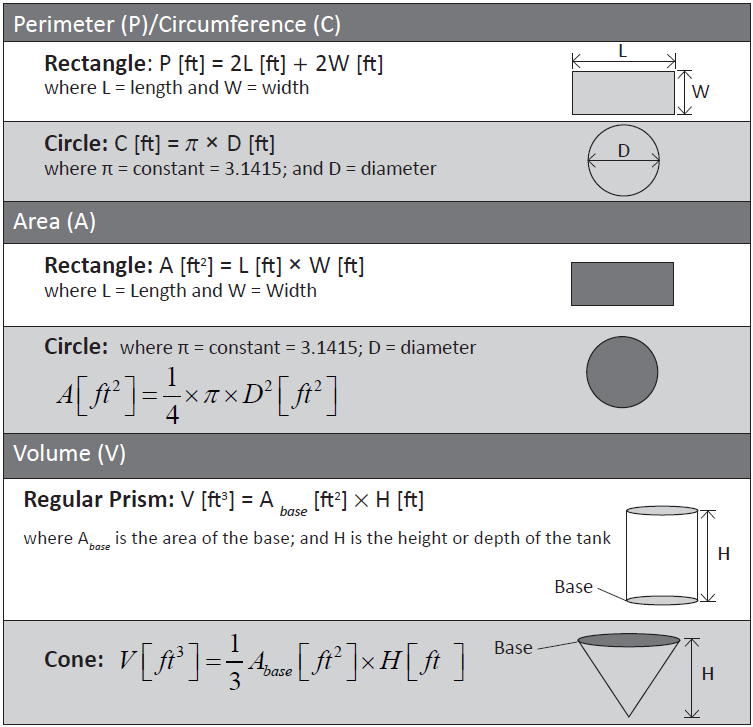
\includegraphics[scale=0.5]{Area&VolumeFormula}
\caption{Area and volume formulas}
\end{center}
\end{table}

\subsection{Example Problems}
% \hl{Example Problems}\\
\begin{enumerate}

\item The floor of a rectangular building is 20 feet long by 12 feet wide and the inside walls are 10 feet high. Find the total surface area of the inside walls of this building\\
Solution:\\
% \begin{center}
\begin{tikzpicture}
	%%% Edit the following coordinate to change the shape of your
	%%% cuboid
      
	%% Vanishing points for perspective handling
	\coordinate (P1) at (-7cm,1.5cm); % left vanishing point (To pick)
	\coordinate (P2) at (8cm,1.5cm); % right vanishing point (To pick)

	%% (A1) and (A2) defines the 2 central points of the cuboid
	\coordinate (A1) at (0em,0cm); % central top point (To pick)
	\coordinate (A2) at (0em,-2cm); % central bottom point (To pick)

	%% (A3) to (A8) are computed given a unique parameter (or 2) .8
	% You can vary .8 from 0 to 1 to change perspective on left side
	\coordinate (A3) at ($(P1)!.8!(A2)$); % To pick for perspective 
	\coordinate (A4) at ($(P1)!.8!(A1)$);

	% You can vary .8 from 0 to 1 to change perspective on right side
	\coordinate (A7) at ($(P2)!.7!(A2)$);
	\coordinate (A8) at ($(P2)!.7!(A1)$);

	%% Automatically compute the last 2 points with intersections
	\coordinate (A5) at
	  (intersection cs: first line={(A8) -- (P1)},
			    second line={(A4) -- (P2)});
	\coordinate (A6) at
	  (intersection cs: first line={(A7) -- (P1)}, 
			    second line={(A3) -- (P2)});

	%%% Depending of what you want to display, you can comment/edit
	%%% the following lines

	%% Possibly draw back faces

	\fill[gray!40] (A2) -- (A3) -- (A6) -- (A7) -- cycle; % face 6
	\node at (barycentric cs:A2=1,A3=1,A6=1,A7=1) {\tiny Floor=W*L};
	
	\fill[gray!50] (A3) -- (A4) -- (A5) -- (A6) -- cycle; % face 3
	\node at (barycentric cs:A3=1,A4=1,A5=1,A6=1) {\tiny Wall - W*H};
	
	\fill[gray!10, opacity=0.2] (A5) -- (A6) -- (A7) -- (A8) -- cycle; % face 4
	\node at (barycentric cs:A5=1,A6=1,A7=1,A8=1) {\tiny Wall - L*H};
	
	\fill[gray!10,opacity=0.5] (A1) -- (A2) -- (A3) -- (A4) -- cycle; % f2
	\node at (barycentric cs:A1=1,A2=1,A3=1,A4=1) {\tiny Wall - L*H};
	
	\fill[gray!40,opacity=0.2] (A1) -- (A4) -- (A5) -- (A8) -- cycle; % f5
	\node at (barycentric cs:A1=1,A4=1,A5=1,A8=1) {\tiny Ceiling=W*L};	
	
	\draw[thick,dashed] (A5) -- (A6);
	\draw[thick,dashed] (A3) -- (A6);
	\draw[thick,dashed] (A7) -- (A6);

	%% Possibly draw front faces

	%\fill[orange] (A1) -- (A8) -- (A7) -- (A2) -- cycle; % face 1
	\node at (barycentric cs:A1=1,A8=1,A7=1,A2=1) {\tiny Wall - W*H};
	


	%% Possibly draw front lines
	\draw[thick] (A1) -- (A2);

	\draw[<->] (-1.8,0.38) -- (-1.8,-1.3)node [midway, above=-1.8mm] {\hspace{-1.3cm}\tiny Height=10'};
	\draw[<->] (-1.6,-1.4) -- (-.3,-2.1)node [midway, above=-2.6mm] {\hspace{-1.3cm}\tiny Length=20'};
	\draw[<->] (2.6,-1.13) -- (0.2,-2.2)node [midway, below=.6mm] {\hspace{1.2cm}\tiny Width=12'};
	\draw[thick] (A3) -- (A4);
	\draw[thick] (A7) -- (A8);
	\draw[thick] (A1) -- (A4);
	\draw[thick] (A1) -- (A8);
	\draw[thick] (A2) -- (A3);
	\draw[thick] (A2) -- (A7);
	\draw[thick] (A4) -- (A5);
	\draw[thick] (A8) -- (A5);
	
	% Possibly draw points
	% (it can help you understand the cuboid structure)
%	\foreach \i in {1,2,...,8}
%	{
%	  \draw[fill=black] (A\i) circle (0.15em)
%	    node[above right] {\tiny \i};
%	}
	% \draw[fill=black] (P1) circle (0.1em) node[below] {\tiny p1};
	% \draw[fill=black] (P2) circle (0.1em) node[below] {\tiny p2};
\end{tikzpicture}\\
% \end{center}
2 Walls W*H + 2 Walls L*H= $2*12*10ft^2 + 2*20*10ft^2$\\
$=240+400=\boxed{640ft^2}$\\

2 Walls W*H + 2 Walls L*H + Floor + Ceiling= $2*12*10ft^2 + 2*20*10ft^2 + 2*12*20ft^2$\\
$=240+400+480=\boxed{1,120ft^2}$\\
\vspace{0.3cm}
\item How many gallons of paint will be required to paint the inside walls of a 40 ft long x 65 ft wide x 20 ft high tank if the paint coverage is 150 sq. ft per gallon.  Note:  We are painting walls only.  Disregard the floor and roof areas.\\
Solution:\\
\vspace{0.3cm}
% \begin{center}
\begin{tikzpicture}
	%%% Edit the following coordinate to change the shape of your
	%%% cuboid
      
	%% Vanishing points for perspective handling
	\coordinate (P1) at (-7cm,1.5cm); % left vanishing point (To pick)
	\coordinate (P2) at (8cm,1.5cm); % right vanishing point (To pick)

	%% (A1) and (A2) defines the 2 central points of the cuboid
	\coordinate (A1) at (0em,0cm); % central top point (To pick)
	\coordinate (A2) at (0em,-2cm); % central bottom point (To pick)

	%% (A3) to (A8) are computed given a unique parameter (or 2) .8
	% You can vary .8 from 0 to 1 to change perspective on left side
	\coordinate (A3) at ($(P1)!.8!(A2)$); % To pick for perspective 
	\coordinate (A4) at ($(P1)!.8!(A1)$);

	% You can vary .8 from 0 to 1 to change perspective on right side
	\coordinate (A7) at ($(P2)!.7!(A2)$);
	\coordinate (A8) at ($(P2)!.7!(A1)$);

	%% Automatically compute the last 2 points with intersections
	\coordinate (A5) at
	  (intersection cs: first line={(A8) -- (P1)},
			    second line={(A4) -- (P2)});
	\coordinate (A6) at
	  (intersection cs: first line={(A7) -- (P1)}, 
			    second line={(A3) -- (P2)});

	%%% Depending of what you want to display, you can comment/edit
	%%% the following lines

	%% Possibly draw back faces

	\fill[gray!40] (A2) -- (A3) -- (A6) -- (A7) -- cycle; % face 6
	\node at (barycentric cs:A2=1,A3=1,A6=1,A7=1) {};
	
	\fill[gray!50] (A3) -- (A4) -- (A5) -- (A6) -- cycle; % face 3
	\node at (barycentric cs:A3=1,A4=1,A5=1,A6=1) {\tiny Wall - W*H};
	
	\fill[gray!10, opacity=0.2] (A5) -- (A6) -- (A7) -- (A8) -- cycle; % face 4
	\node at (barycentric cs:A5=1,A6=1,A7=1,A8=1) {\tiny Wall - L*H};
	
	\fill[gray!10,opacity=0.5] (A1) -- (A2) -- (A3) -- (A4) -- cycle; % f2
	\node at (barycentric cs:A1=1,A2=1,A3=1,A4=1) {\tiny Wall - L*H};
	
	\fill[gray!40,opacity=0.2] (A1) -- (A4) -- (A5) -- (A8) -- cycle; % f5
	\node at (barycentric cs:A1=1,A4=1,A5=1,A8=1) {};	
	
	\draw[thick,dashed] (A5) -- (A6);
	\draw[thick,dashed] (A3) -- (A6);
	\draw[thick,dashed] (A7) -- (A6);

	%% Possibly draw front faces

	%\fill[orange] (A1) -- (A8) -- (A7) -- (A2) -- cycle; % face 1
	\node at (barycentric cs:A1=1,A8=1,A7=1,A2=1) {\tiny Wall - W*H};
	


	%% Possibly draw front lines
	\draw[thick] (A1) -- (A2);

	\draw[<->] (-1.8,0.38) -- (-1.8,-1.3)node [midway, above=-1.8mm] {\hspace{-1.3cm}\tiny Height=20'};
	\draw[<->] (-1.6,-1.4) -- (-.3,-2.1)node [midway, above=-2.6mm] {\hspace{-1.3cm}\tiny Length=45'};
	\draw[<->] (2.6,-1.13) -- (0.2,-2.2)node [midway, below=.6mm] {\hspace{1.2cm}\tiny Width=65'};
	\draw[thick] (A3) -- (A4);
	\draw[thick] (A7) -- (A8);
	\draw[thick] (A1) -- (A4);
	\draw[thick] (A1) -- (A8);
	\draw[thick] (A2) -- (A3);
	\draw[thick] (A2) -- (A7);
	\draw[thick] (A4) -- (A5);
	\draw[thick] (A8) -- (A5);
	
	% Possibly draw points
	% (it can help you understand the cuboid structure)
%	\foreach \i in {1,2,...,8}
%	{
%	  \draw[fill=black] (A\i) circle (0.15em)
%	    node[above right] {\tiny \i};
%	}
	% \draw[fill=black] (P1) circle (0.1em) node[below] {\tiny p1};
	% \draw[fill=black] (P2) circle (0.1em) node[below] {\tiny p2};
\end{tikzpicture}\\
% \end{center}
\vspace{0.3cm}
2 Walls W*H + 2 Walls L*H = $2*65*20ft^2 + 2*40*20ft^2= 2,600+1,600=4,200ft^2$\\
$\implies @150\dfrac{ft^2}{gal} \enspace paint \enspace coverage \enspace \rightarrow \enspace \dfrac{4,200\cancel{ft^2}}{150\dfrac{\cancel{ft^2}}{gal}}=\boxed{28 \enspace gallons}$
\vspace{0.3cm}
\item What is the circumference of a 100 ft diameter circular clarifier?\\
\vspace{0.3cm}
Solution:\\
\vspace{0.3cm}
$Circumference=\pi*D=3.14*100ft=\boxed{314ft}$
\vspace{0.3cm}
\item If the surface area of a clarifier is 5,025$ft^2$, what is its diameter?\\
\vspace{0.3cm}
Solution:\\
\vspace{0.3cm}
$Surface \enspace area=\dfrac{\pi}{4}*D^2 \enspace \implies 5025(ft^2)=0.785*D^2 (ft^2)$\\
$\implies D^2=\dfrac{5025}{0.785} \implies D=\sqrt{6401.3}=\boxed{80ft}$
\vspace{0.3cm}

\item How many gallons of wastewater would 600 feet of 6-inch diameter pipe hold, approximately?\\
\vspace{0.3cm}
Solution:\\

\vspace{0.3cm}
% \begin{center}
\begin{tikzpicture}
\draw (0,0) ellipse (0.1cm and 0.3cm);
\draw (10,0) ellipse (0.1cm and 0.3cm);
\draw [-] (0,-0.29) -- (10,-0.29);
\draw [-] (0,0.29) -- (10,0.29);
\draw [<->] (10,-0.28) -- (10,0.28) node [midway, below=-3mm] {\hspace{2.6cm}Diameter=6"};
\draw [<->] (0,-.68) -- (10,-.68)node [midway, below] {\hspace{0.9cm}Length=600'};
\end{tikzpicture}
% \end{center}
\vspace{0.3cm}
$Volume=\dfrac{\pi}{4}D^2*L=0.785*\Big(\dfrac{6}{12}\Big)^2*600\cancel{ft^3}*7.48\dfrac{gallons}{\cancel{ft^3}}=\boxed{881 \enspace gallons}$
\vspace{0.5cm}
\item A 110 ft diameter digester with a 12 ft deep cone is operated at a side water depth of 20 ft.  Caluclate the volume of sludge in the digester in $ft^3$ and gallons.\\
\vspace{0.3cm}
Solution:\\
\vspace{0.3cm}
% \begin{center}
\begin{tikzpicture}
\draw (0,0) ellipse (2cm and 0.3cm);
\draw (0,-2.3) ellipse (2cm and 0.3cm);
\draw (0,-.8) ellipse (2cm and 0.3cm);
\draw [-] (2,-2.3) -- (2,0);
\draw [<->] (-2,0) -- (2,0) node [midway, below=-0.9cm] {\hspace{0.9cm}Diameter (D)=110'}; 
\draw [<->] (-2.6,-2.3) -- (-2.6,0) node [midway, below=-.3cm] {\hspace{-2.6cm}Cylinder Height};
\draw [<->] (2.5,-2.3) -- (2.5,-0.8) node [midway, below=-0.2cm] {\hspace{5.2cm}Side Water Depth (SWD) =20'};
\draw [-] (0,-4) -- (2,-2.3);
\draw [-] (0,-4) -- (-2,-2.3);
\draw [-] (0,-4) -- (2,-2.3);
\draw [-] (-2,0) -- (-2,-2.3);
\draw [<->] (2.5,-2.3) -- (2.5,-4)node [midway, below=-0.4cm] {\hspace{3.8cm}Cone Depth (CD)=12'};
\end{tikzpicture}\\
% \end{center}
$Digester \enspace volume=Volume_{cylinder}+Volume_{cone}$\\
$\implies Digester \enspace volume=\dfrac{\pi}{4}D^2*SWD+\dfrac{1}{3}*\Bigg(\dfrac{\pi}{4}*D^2*CD\Bigg)$\\
\vspace{0.3cm}
$=0.785*110^2*20+1.05*110^2*12=\boxed{227,988ft^3}$\\
\vspace{0.3cm}
$227,988\cancel{ft^3}*7.48\dfrac{gallons}{\cancel{ft^3}}=\boxed{1,705,352 \enspace gallons}$
\end{enumerate}

\section{Pounds Formula}



Pounds formula is used for:
\begin{itemize}
\item Calculating the quantity in pounds of a particular wastewater constituent entering or leaving a wastewater treatment process
\item Calculating the pounds of chemicals to be added\\
\end{itemize}
So if the concentration of a particular constituent (in mg/liter) and the volume or flow of wastewater is given, one can calculate the amount of that constituent in pounds using the following – Pounds Formula:
$$lbs \enspace \textbf{or} \enspace \dfrac{lbs}{day}=concentration(\dfrac{mg}{l})*8.34*volume(MG) \enspace \textbf{or} \enspace flow(\dfrac{MG}{day}(MGD)$$

\begin{figure}[h!]
\begin{center}
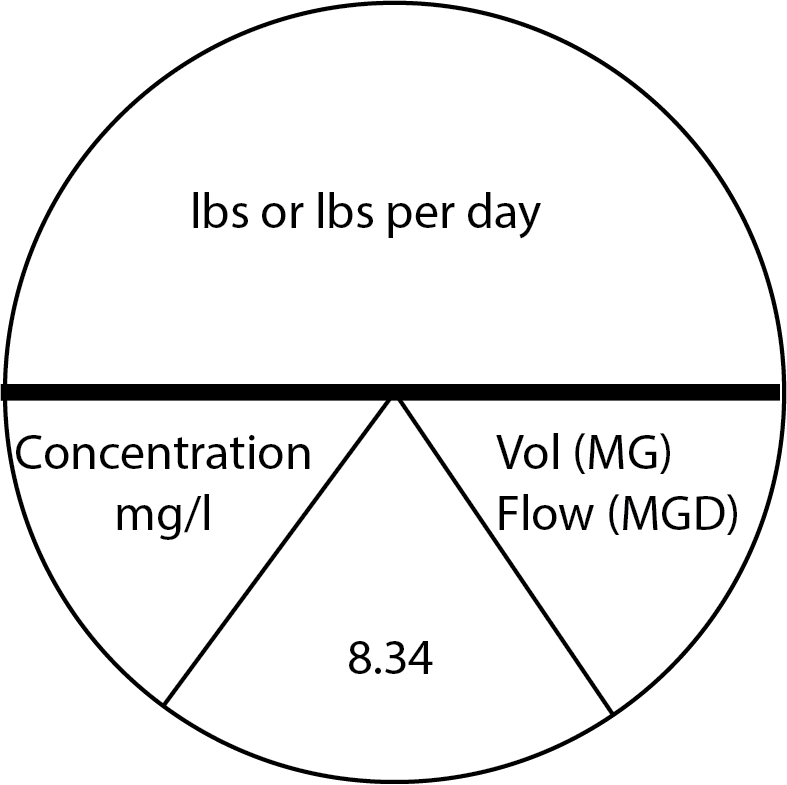
\includegraphics[scale=0.5]{PoundsFormula}
\end{center}
\caption{Pounds formula "nomograph"}
\end{figure}
\vspace{0.3cm}
There are three variables – (lbs, concentration and volume) and one constant (8.34) in the pounds formula.  Knowing any of the two variables in the formula, one can calculate the third (unknown) variable by rearranging the equation.


\newpage
\subsection{Concentration}\index{Concentration}

Concentration is typically expressed as mg/l which is the weight of the constituent (mg) in one  liter of solution (wastewater).  As one liter of water weighs one-million mg, a concentration of 1 mg/l implies 1 mg of constituent per 1 million mg of water or one part per million (ppm). \\ \textbf{Thus, mg/l and ppm are synonymous.}\\  
\vspace{6pt}
Sometimes the constituent concentration is expressed in terms of percentage.\\
\vspace{6pt}
For example:  sludge containing 5\% solids or a 12.5\% chlorine concentration solution.\\
\vspace{6pt}
As one liter of water weighs 1,000,000 mg, one percent of that weight is 10,000 mg.  \texthl{So 1\% solids implies 10,000 mg of solids per liter or 10,000 mg/l or 10,000 ppm.}\\
\vspace{6pt}
$1\%  \enspace concentration = 10,000 \enspace ppm \enspace or \enspace\dfrac{mg}{l}$\\
\vspace{4pt}
$0.1\% \enspace  concentration = 1,000 \enspace ppm \enspace or \enspace \dfrac{mg}{l}$\\
\vspace{4pt}
$0.01\% \enspace  concentration = 100 \enspace ppm \enspace or \enspace \dfrac{mg}{l}$\\
\vspace{4pt}
$10\% \enspace concentration = 100,000 \enspace ppm \enspace or \enspace \dfrac{mg}{l}$\\
\vspace{4pt}
$5\% \enspace  concentration = 50,000 \enspace ppm \enspace or \enspace \dfrac{mg}{l}$\\
\vspace{4pt}
$12.5\% \enspace  concentration = 125,000 \enspace ppm \enspace or \enspace \dfrac{mg}{l}$\\
\vspace{0.5cm}
\subsection{Example Problems}
% \hl{Example Problems}\\
\begin{enumerate}[1.]
\item Calculate the lbs/day of solids entering the plant given the influent flow is 5 MGD with an average solids concentration  of 250 mg/l.\\
\vspace{0.5cm}
Solution:\\
\vspace{0.5cm}
Applying lbs formula:\\
$\dfrac{lbs}{day}=5 MGD *250\dfrac{mg}{l}*8.34 = \boxed{10,425\dfrac{lbs}{day}}$
\\
\vspace{6pt}
\item Calculate the lbs of solids in the primary sludge if the sludge flow is 7500 gallons and the solids concentration is 4.5\%.\\
\vspace{0.5cm}
Solution:\\
\vspace{0.5cm}
Applying lbs formula:\\
\vspace{0.5cm}
$lbs \enspace solids = \dfrac{7500}{1,000,000}MG * 4.5*10,000 *8.34 = \boxed{2,815 \enspace lbs \enspace solids}$\\
\textbf{Note:}\\  
1) 7500 gallons was converted to MG by dividing by 1,000,000\\
\vspace{0.5cm}
$7500 \enspace gallons * \dfrac{1 MG}{1,000,000 \enspace gallon}$\\
\vspace{0.5cm}
2) 4.5\% was converted to mg/l by multiplying by 10,000 as 1\%=10,000mg/l
\end{enumerate}


\section{Process Removal Efficiency Calculations}\index{Process Removal Efficiency Calculations}

\begin{itemize}
\item Process removal rate or removal efficiency is the percentage of the inlet concentration removed.  
\item It is used for quantifying the pollutant removal during wastewater treatment and is established based upon the amount of a particular wastewater constituent entering and leaving a treatment process.

\item $Process \enspace Removal \enspace Rate \enspace (\%) = \dfrac{Pollutant \enspace  In-Pollutant\enspace  Out}{Pollutant \enspace In}*100$\\

\item If 10 units of a pollutant are entering a process and 8 units of pollutant are leaving (process removes 2 units), then the process removal rate for that pollutant is (10-8)/10*100=20\%.  In this example the process is 20\% efficient in removing that particular pollutant.

\item The amount of pollutant can be measured in terms of concentration (mg/l) or in terms of mass loading (lbs).  The pounds formula is used for calculating the mass loadings.  
\end{itemize}
The above example is for calculating the removal efficiency using the inlet and outlet concentrations or mass loading.\\
The methods below can be used for calculating either the inlet or outlet pollutant concentrations, if the removal efficiency and the corresponding inlet or outlet concentrations are given. 


\hl{Case 1:  Calculating outlet conc. (X) given the inlet conc. and removal efficiency (RE\%):}

\tikzstyle{block} = [rectangle, draw, fill=red!40, 
    text width=6em, text centered, rounded corners, minimum height=3em]
\tikzstyle{arrow} = [draw, -latex']
\begin{figure}[!h]
\centering
\begin{tikzpicture}[node distance =1.5cm, auto]
    \draw ++(0,0) node [block] (Process) {Process};
   \node[node distance=1.9in] (dummy_in) [left of=Process] {In};
   \node[node distance=1.9in] (dummy_out) [right of=Process] {Out};
	\node (Removal) [below of=Process, yshift=-0in] {$\tiny{Removal \enspace Efficiency=RE\% \enspace (Given)}$};
    \path [arrow] (dummy_in)-- (Process)  node [above] {\hspace{-5.8cm}$A \enspace mg/l \enspace (Given) $} node [below] {\hspace{-5.8cm}$100 \enspace mg/l$};
    \path [arrow] (Process) -- (dummy_out)  node [above] {\hspace{-4cm}$X \enspace mg/l \enspace (Unknown)$} node [below] {\hspace{-3.9cm}($100-RE\%)\enspace mg/l$};
   \draw[arrow] (Process) -- (Removal);
\end{tikzpicture}
\end{figure}
Using the fact that if the inlet concentration was 100 mg/l, the outlet concentration would be 100 minus the removal efficiency.\\
Setup the equation as:  $\dfrac{Out}{In}: \enspace \dfrac{X \enspace mg/l}{A \enspace mg/l}=\dfrac{100-RE\%}{100}$\\
Calculate X using cross multiplication - if $\dfrac{A}{B}=\dfrac{C}{D} \implies A=B*\dfrac{C}{D}$:\\
$X \enspace mg/l=A \enspace mg/l*\dfrac{100-RE\%}{100}$\\

\hl{Case 2:  Calculating inlet conc. (X) given the outlet conc. and removal efficiency (RE\%):}

\begin{figure}[!h]
\centering
\begin{tikzpicture}[node distance =1.5cm, auto]
    \draw ++(0,0) node [block] (Process) {Process};
   \node[node distance=1.9in] (dummy_in) [left of=Process] {In};
   \node[node distance=1.9in] (dummy_out) [right of=Process] {Out};
	\node (Removal) [below of=Process, yshift=-0in] {$Removal \enspace Efficiency=RE\% \enspace (Given)$};
    \path [arrow] (dummy_in)-- (Process)  node [above] {\hspace{-5.8cm}$X \enspace mg/l \enspace (Unknown)$} node [below] {\hspace{-5.8cm}$100 \enspace mg/l$};
    \path [arrow] (Process) -- (dummy_out)  node [above] {\hspace{-4cm}$A \enspace mg/l \enspace (Given)$} node [below] {\hspace{-3.9cm}($100-RE\%)\enspace mg/l$};
   \draw[arrow] (Process) -- (Removal);
\end{tikzpicture}
\end{figure}
Using the fact that if the inlet concentration was 100 mg/l, the outlet concentration would be 100 minus the removal efficiency.\\
Setup the equation as:  $\dfrac{In}{Out}: \enspace \dfrac{X \enspace mg/l}{A \enspace mg/l}=\dfrac{100}{100-RE\%}$\\
\vspace{0.3cm}
Calculate X using cross multiplication - if $\dfrac{A}{B}=\dfrac{C}{D} \implies A=B*\dfrac{C}{D}$:\\
$X \enspace mg/l=A \enspace mg/l*\dfrac{100}{100-RE\%}$\\

\vspace{0.4cm}
\hl{Example Problems:}\\

\begin{enumerate}

\item What is the \% removal efficiency if the influent concentration is 10 mg/L and the effluent concentration is 2.5 mg/L?\\
$Removal \enspace Rate (\%) = \dfrac{In-Out}{In}*100 \implies \dfrac{10-2.5}{10}*100=\boxed{75\%}$



\item Calculate the outlet concentration if the inlet concentration is 80 mg/l and the process removal efficiency is 60\%\\
Solution:\\

\tikzstyle{block} = [rectangle, draw, fill=red!40, 
    text width=6em, text centered, rounded corners, minimum height=3em]
\tikzstyle{arrow} = [draw, -latex']
\begin{figure}[!h]
\centering
\begin{tikzpicture}[node distance =1.5cm, auto]
    \draw ++(0,0) node [block] (Process) {Process};
   \node[node distance=1.5in] (dummy_in) [left of=Process] {In};
   \node[node distance=1.5in] (dummy_out) [right of=Process] {Out};
	\node (Removal) [below of=Process, yshift=-0in] {$Removal \enspace Efficiency=60\%$};
    \path [arrow] (dummy_in)-- (Process)  node [above] {\hspace{-4.39cm}$80mg/l$} node [below] {\hspace{-4.39cm}$100mg/l$};
    \path [arrow] (Process) -- (dummy_out)  node [above] {\hspace{-3.cm}$Xmg/l$} node [below] {\hspace{-3cm}40mg/l};
   \draw[arrow] (Process) -- (Removal);
\end{tikzpicture}
%\caption[MFCC]{Diagrama en bloques del cálculo de las MFCC para un frame.}
%\label{MFCC}
\end{figure}

$\dfrac{Out}{In} \enspace:\enspace\dfrac{Actual \enspace Outlet (X)}{80}=\dfrac{100-60}{100}$\\
$\implies \dfrac{Actual \enspace Outlet (X)}{80} =0.4$\\
$\implies Actual \enspace  Outlet (X) = 0.4 * 80 = \boxed{32 mg/l}$\\


\item Calculate the inlet concentration if the outlet concentration is 80 mg/l and the process removal efficiency is 60\%\\

\tikzstyle{block} = [rectangle, draw, fill=red!40, 
    text width=6em, text centered, rounded corners, minimum height=3em]
\tikzstyle{arrow} = [draw, -latex']
\begin{figure}[!h]
\centering
\begin{tikzpicture}[node distance =1.5cm, auto]
    \draw ++(0,0) node [block] (Process) {Process};
   \node[node distance=1.5in] (dummy_in) [left of=Process] {In};
   \node[node distance=1.5in] (dummy_out) [right of=Process] {Out};
	\node (Removal) [below of=Process, yshift=-0in] {$Removal \enspace Efficiency=60\%$};
    \path [arrow] (dummy_in)-- (Process)  node [above] {\hspace{-4.39cm}$Xmg/l$} node [below] {\hspace{-4.39cm}$100mg/l$};
    \path [arrow] (Process) -- (dummy_out)  node [above] {\hspace{-3.cm}80mg/l} node [below] {\hspace{-3cm}40mg/l};
   \draw[arrow] (Process) -- (Removal);
\end{tikzpicture}
\end{figure}

$\dfrac{In}{Out} \enspace : \enspace \dfrac{Actual \enspace inlet \enspace  (X)}{80}=\dfrac{100}{100-60}\implies \dfrac{Actual \enspace inlet \enspace  (X)}{80}=2.5$\\    
Rearranging the equation:   $Actual \enspace inlet (X)=2.5*80 = \boxed{200 mg/l}$\\

\item If a plant removes 35\% of the influent BOD in the primary treatment and 85\% of the remaining BOD in the secondary system, what is the BOD of the raw wastewater if the BOD of the final effluent is 20mg/l\\
Solution:\\

\begin{figure}[!h]
\centering
\begin{tikzpicture}[node distance =1.5cm, auto]
    \draw ++(0,0) node [block] (Primary) {Primary};
    
   \node[node distance=1.9in] (dummy_in) [left of=Primary] {Influent BOD};
   \node[node distance=1.9in] (dummy_out) [right of=Primary] {Primary BOD Out};
	\node (Removal) [below of=Primary, yshift=-0in] {$Removal \enspace Efficiency=35\% $};
    \path [arrow] (dummy_in)-- (Primary)  node [above] {\hspace{-4.8cm}$X \enspace mg/l \enspace$} node [below] {};
    \path [arrow] (Primary) -- (dummy_out)  node [above] {\hspace{-4.9cm}$0.65X \enspace mg/l$} node [below] {};
   \draw[arrow] (Process) -- (Removal);
\end{tikzpicture}
\end{figure}


\begin{figure}[!h]
\centering
\begin{tikzpicture}[node distance =1.5cm, auto]
    \draw ++(0,0) node [block] (Secondary) {Secondary};
    
   \node[node distance=1.9in] (dummy_in) [left of=Secondary] {Primary BOD Out};
   \node[node distance=1.9in] (dummy_out) [right of=Secondary] {Secondary BOD Out};
	\node (Removal) [below of=Secondary, yshift=-0in] {$Removal \enspace Efficiency=85\% $};
    \path [arrow] (dummy_in)-- (Secondary)  node [above] {\hspace{-4.8cm}$0.65X \enspace mg/l \enspace$} node [below] {\hspace{-5cm}$100 \enspace mg/l$};
    \path [arrow] (Secondary) -- (dummy_out)  node [above] {\hspace{-4.9cm}$20 \enspace mg/l$} node [below] {\hspace{-4.9cm}$15 \enspace mg/l$};
   \draw[arrow] (Process) -- (Removal);
\end{tikzpicture}
\end{figure}
\vspace{0.3cm}
For the Secondary process:\\
$\dfrac{In}{Out}: \enspace \dfrac{0.65X}{20}=\dfrac{100}{15} \implies X \enspace mg/l=\dfrac{100*20}{15*0.65}=\boxed{205 \enspace mg/l}$\\

\vspace{0.3cm}
Alternate Solution \#1

$\xrightarrow[
				\text{X}\dfrac{mg}{l}
			]
			{
			\text{Influent BOD}
			}
 \boxed{Primary}
 \xrightarrow[
 				\text{X-0.35X=X*(1-0.35)=0.65X}\dfrac{mg}{l}
 			]
 			{
 			\text{Primary Effluent BOD}
 			}
 \boxed{Secondary}
 \xrightarrow[
				\text{0.65X-0.5525X=(0.65-0.5525)X=0.0975X }
			 ]
			{
			\text{Secondary Effluent BOD}
			}
$\\
\hspace{2.8cm}$\downarrow$ {\tiny(0.35X)BOD Removed}\hspace{3.2cm}$\downarrow$ {\tiny(0.65*0.85)X = 0.5525X BOD Removed}\\
$\implies 0.0975X=20 \implies X=\dfrac{20}{0.0975}=\boxed{205\dfrac{mg}{l}}$\\

\vspace{0.3cm}

Alternate Solution \#2:\\
$\xrightarrow[\text{X}\dfrac{mg}{l}]{\text{Influent BOD}}\boxed{Primary}\xrightarrow[\text{0.65X}]{\text{Primary Effluent BOD}}\boxed{Secondary}\xrightarrow[\text{(0.65*0.15)X}]{\text{Secondary Effluent BOD}}$\\
\hspace{2.8cm}$\downarrow$ {\tiny(0.35X)BOD Removed}\hspace{2.2cm}$\downarrow$ {\tiny(0.65X*0.85)BOD Removed}\\

Primary Effluent BOD = Influent BOD * (1-Primary BOD Removal), and\\
Secondary Effluent BOD=[Primary Effluent BOD]*(1-Secondary BOD Removal)\\
Secondary Eff. BOD=[Influent BOD * (1-Primary BOD Removal)]*(1-Secondary BOD Removal)\\

Therefore, 20 = [X*(1-0.35)] * (1-0.85)= X*0.65*0.15\\
$\implies 20 \enspace \dfrac{mg}{l}= 0.0975X \implies X=\dfrac{20}{0.0975}=\boxed{205 \enspace \dfrac{mg}{l}}$\\

\end{enumerate}

\section{Preliminary Treatment Calculations}\index{Preliminary Treatment Calculations}

\subsection{Channel Velocity and Flow Rate}\index{Channel Velocity and Flow Rate}
Flow Rate - Q (volume/time) = velocity (distance or length traveled /time) * surface area\\
Velocity is the speed at which the water is flowing.  It is measured in units of length/time – ft./sec.\\
Velocity of water flowing through can be calculated by dividing the flow rate by area of the flow stream.\\
\vspace{0.5cm}
$Velocity \enspace \dfrac{length}{time}= \dfrac{flow \enspace rate(\dfrac{volume \enspace or \enspace cubic \enspace length}{time})}{surface \enspace area \enspace in \enspace the \enspace direction \enspace of \enspace flow-square \enspace length}$\\
\newpage
\textbf{For a flow in a channel:}\\
\vspace{0.5cm}
\hl{Example Problems:}\\
\begin{enumerate}[1.]
\item Calculate the velocity of a 14 MGD flow in a 6 ft wide channel with a water depth of two feet.\\
\begin{center}
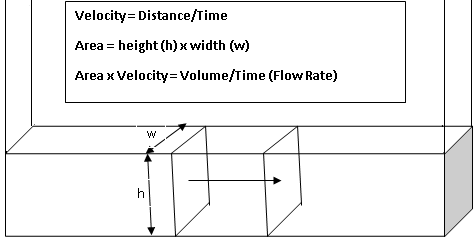
\includegraphics[scale=0.5]{ChannelFlow3}
\end{center}
$Flow (Q) = Velocity (V) * Area (A)$\\
$\implies 14 \dfrac{MG}{day}* \dfrac{10^6 gal}{MG} * \dfrac{ft^3}{7.48 gal}*\dfrac{day}{24*60*60} = V \dfrac{ft}{sec}* 6 ft * 2 ft \implies 21.7 \dfrac{ft^3}{sec}= 12V\dfrac{ft^3}{sec}$\\
$\implies V \dfrac{ft}{sec}= \dfrac{21.7}{12}= \boxed{1.8\dfrac{ft}{sec}}$\\

\item Calculate the flow, in gpd, that would pass through a grit chamber 2 feet wide, at a depth of 6 inches, with a velocity of 1 ft /sec\\
Solution:\\
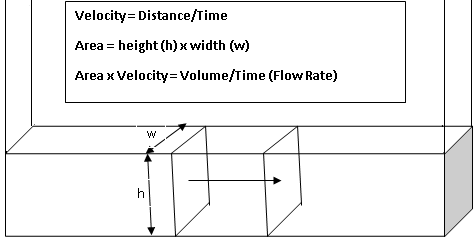
\includegraphics[scale=0.5]{ChannelFlow3}\\
$Q=V*A$\\
$Q=1\dfrac{ft}{s}*(2*0.5)ft^2=1\dfrac{ft^3}{s}$\\
$Q=1\dfrac{\cancel{ft^3}}{\cancel{s}}*\dfrac{(1440*60)\cancel{s}}{day}*7.48\dfrac{gal}{\cancel{ft^3}}=\boxed{646,272\dfrac{gal}{day}}$
\vspace{0.5cm}
\item A wastewater channel is 3.25 feet wide and is conveying a wastewater flow of 3.5 MGD. The wastewater flow is 8 inches deep. Calculate the velocity of this flow.\\
Solution:\\
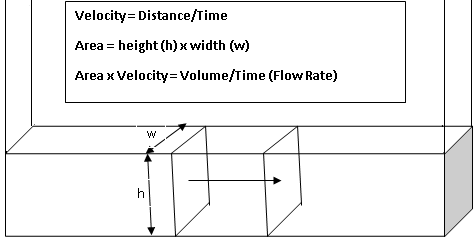
\includegraphics[scale=0.5]{ChannelFlow3}\\
$Q=V*A \implies V=\dfrac{Q}{A}$\\
$\implies V\dfrac{ft}{s}=\dfrac{3.5\dfrac{\cancel{MG}}{\cancel{day}}*\dfrac{1000000\cancel{gal}}{\cancel{MG}}*\dfrac{ft^{\cancel{3}}}{7.48\cancel{gal}}*\dfrac{\cancel{day}}{(1440*60)s}}{(3.25*0.75)\cancel{ft^2}}=\boxed{2.2\dfrac{ft}{s}}$
\vspace{0.5cm}
\item A plastic float is dropped into a wastewater channel and is found to travel 10 feet in 4.2 seconds. The channel is 2.4 feet wide and is flowing 1.8 feet deep. Calculate the flow rate of this wastewater in cubic feet per second.\\
Solution:\\
$Q=V*A$\\
$\implies Q\Big(\dfrac{ft^3}{s}\Big)=\dfrac{10ft}{4.2s}*(2.4*1.8)ft^2=\boxed{10.3\dfrac{ft^3}{s}}$
\end{enumerate}

\subsection{Grit Removal Rates}\index{Grit Removal Rates}
\emph{Typical grit removal ranges from 0.5 to 30 ft$^3$/MG}\\
\vspace{0.3cm}
\hl{Example Problems:}\\
\begin{enumerate}[1.]
\item At a wastewater treatment plant which receives a flow rate of 650,000 gallons per day, a total of 50 cubic feet of grit was removed for the month. Calculate the rate of grit removal assuming 30 days in a month.\\
Solution:\\
$Grit Removal\dfrac{ft^3}{MG}=50\dfrac{ft^3}{ \cancel{month}}*\dfrac{\cancel{month}}{30\cancel{days}}*\dfrac{\cancel{day}}{650,000\cancel{gal}}*1,000,000\dfrac{\cancel{gal}}{MG}=\boxed{2.6\dfrac{ft^3}{MG}}$
\end{enumerate}

\section{Primary Treatment Calculations}\index{Primary Treatment Calculations}

\subsection{Hydraulic or Surface Loading Rate}\index{Hydraulic or Surface Loading Rate}

The hydraulic or surface loading rate measures how rapidly wastewater moves through the primary clarifier.  It is measured in terms of the number of gallons flowing each day through one square foot surface area of the clarifier. 
$$Clarifier \enspace hydraulic \enspace loading \enspace 	\Big(\dfrac{gpd}{ft^2}\Big) =\dfrac{Clarifier \enspace influent 	\enspace flow (gpd)}{Clarifier \enspace surface \enspace area 	(ft^2)}$$ 
		Rectangular clarifier surface area  = width * length\\
		Circular clarifier surface area  = 0.785 * Diameter$^2 $\\
\subsection{Detention Time}\index{Detention Time}

Detention time is the length of time that wastewater stays in the settling tank is called the detention time.  It is also the time it takes for a unit volume of wastewater to pass entirely through a primary clarifier\\
$$Clarifier \enspace detention \enspace time \enspace (hr) = 	\dfrac{ Clarifier \enspace volume (cu.ft \enspace or \enspace gal)}{Influent \enspace flow \enspace (cu.ft \enspace or \enspace gal)/hr)}$$
Rectangular clarifier volume = width * length * depth of water\\
Circular clarifier volume = 0.785 * Diameter$^2$ * depth of water\\
Typically volume is calculated in cu. ft and influent flow is given in gallons.  Use 7.48 gal/ft$^3$ conversion factor to convert volume in cu. ft to gallons.\\

\subsection{Weir Overflow Rate}\index{Weir Overflow Rate}
The weirs at the end of the primary clarifier allow for the even distribution of the the outlet flow across the entire length of the weir.  An adequate length of weir is needed to ensure smooth and even flow of wastewater over the weirs.  Weir overflow rate measures the number of gallons of wastewater per day flowing over one foot of weir. 

		$$Weir \enspace over \enspace flow \enspace rate \Big(\dfrac{gpd}{ft}\Big) =\Big(\dfrac{Clarifier \enspace influent \enspace  flow (gpd)}{Total \enspace effluent 					\enspace weir \enspace length \enspace (ft)}\Big)$$
		Circular clarifier weir length = 3.14 * Diameter\\

\hl{Example problem for (a), (b) and (c) above:}\\
		\vspace{0.2cm}
A circular clarifier receives a flow of 11 MGD.  If the clarifier is 90 ft. in diameter and is 12 ft. deep, what is: a) the hydraulic/surface loading rate, b) clarifier detention time in hours, and c) weir overflow rate?\\
		\vspace{0.2cm}
a) Hydraulic/surface loading rate:\\
$Clarifier \enspace hydraulic \enspace loading \enspace 	\Big(\dfrac{gpd}{ft^2}\Big) ==\dfrac{\dfrac{11\cancel{MG}}{{day}}*\dfrac{10^6gal}{\cancel{MG}}}{0.785*90^2 ft^2}=\boxed{1,730gpd/ft^2}$\\
		\vspace{0.5cm}
b) Clarifier detention time:\\
$Clarifier \enspace detention \enspace time \enspace (hr) = 	\dfrac{ Clarifier \enspace volume (cu.ft \enspace or \enspace gal)}{Influent \enspace flow \enspace (cu.ft \enspace or \enspace gal)/hr)}$\\
		\vspace{0.2cm}
$Clarifier \enspace detention \enspace time \enspace (hr) = 	\dfrac{(0.785*90^2*15)\cancel{ft^3}}{\dfrac{11\cancel{MG}}{\cancel{day}}*\dfrac{10^6\cancel{gal}}{\cancel{MG}}*\dfrac{\cancel{ft^3}}{7.48\cancel{gal}}*\dfrac{\cancel{day}}{24hrs}}=\boxed{2hrs}$\\
		\vspace{0.5cm}
c) Weir overflow rate:\\
		\vspace{0.2cm} 
$Weir \enspace overflow \enspace rate \Big(\dfrac{gpd}{ft}\Big) =\dfrac{\dfrac{11\cancel{MG}}{{day}}*\dfrac{10^6gal}{\cancel{MG}}}{3.14*90 ft}=\boxed{38,924gpd/ft}$\\

\subsection{Removal Efficiency}\index{Removal Efficiency}		
Primary sedimentation removes suspended wastewater solids which includes BOD.  The efficiency of the primary is established as the percentage of the amount of parameter removed.  The parameter may quantified as mass (lbs) or as concentration (mg/l).

$$Removal \enspace efficiency (\%) = \dfrac{Parameter  \enspace In - Parameter  \enspace Out}{Parameter \enspace In} * 100$$

For TSS removal:\\
$$TSS \enspace Removal \enspace efficiency (\%) = \dfrac{TSS  _{In} \enspace(mg/l)  - TSS_{Out} \enspace(mg/l)  }{TSS _{In} \enspace(mg/l)  } * 100$$

For BOD removal:\\
$$BOD \enspace Removal \enspace efficiency (\%) = \dfrac{BOD_{In} \enspace(mg/l)  - BOD_{Out} \enspace(mg/l)  }{BOD _{In} \enspace(mg/l)  } * 100$$
\subsection{Solids Removal}\index{Solids Removal}	

\hl{\textbf{Type 1 Problems:}  These involve calculating lbs of solids removed given any two of the following TSS parameters - inlet concentration, outlet concentration and removal efficiency.}\\
a. If the inlet and outlet concentrations are given, calculate the mg/l of TSS removed using: 
$$TSS_{removed} = TSS_{in}(mg/l) - TSS_{out} (mg/l) $$
Then knowing the flow, use the lbs formula to calculate the lbs solids removed.

b. If either inlet or outlet concentration is given along with the clarifier removal efficiency, using the removal efficiency calculate the unknown outlet concentration (if only the inlet is given) or the inlet concentration (if only the outlet is given)\\
i) If inlet and removal efficiency is given, calculate the outlet by subtracting the product of inlet and removal efficiency from the inlet.
$$TSS_{out}=TSS_{in} - (TSS_{in}*\%Removal)$$
Example if the removal efficiency is 60\% and the inlet concentration is 300mg/l: $$TSS_{out}=300 - 300*0.6=120mg/l$$
ii) If outlet and removal efficiency is given, calculate the inlet concentration by dividing the outlet by (1-removal efficiency).\\
$$TSS_{in}=\dfrac{TSS_{out}}{1-\%Removal}$$
Example if the removal efficiency is 60\% and the outlet concentration is 120mg/l: $$TSS_{in}=\dfrac{120}{1-0.6}=300mg/l$$ 

Note:  You may derive the above formulas by algebraically manipulating: $\%Removal=\dfrac{TSS_{in} -TSS_{out}}{TSS_{in}}$\\
\hl{Example Problem:}\\
How many lbs of solids are removed daily by a primary clarifier treating a 6 MGD flow if the average influent TSS concentration is 300 mg/l and the clarifier TSS removal efficiency is 67\%.\\
$TSS_{out}=(300mg/l - 300*0.67)=99mg/l$\\
$lbs \enspace solids \enspace  removed = (300-99)mg/l*8.34*6MGD=\boxed{10,058 \enspace lbs \enspace solids \enspace removed \enspace per \enspace day}$\\
\vspace{0.5cm}
\hl{\textbf{Type 2 Problems:}  These involve calculating the amount of sludge pumping given the solids removed.  The solids removed from the primary clarifier is sludge with a typical solids concentration of about 3\% to 5\%.}\\
Given the amount of total solids removed and given the sludge concentration, the volume of sludge pumping can be calculated as follows:  $$\dfrac{ft^3\enspace sludge\enspace pumped}{ day}= \dfrac{lbs \enspace solids \enspace (removed)}{day} * \dfrac{1 \enspace lb \enspace sludge}{(\%)\enspace lbs \enspace solids}*\dfrac{gal \enspace sludge}{8.34lb \enspace sludge}*\dfrac{ft^3 \enspace sludge}{7.48 \enspace gal} $$
So for the solids removed in the above example, if the primary sludge has 5\% solids, the required sludge pumping can be calculated as:
$$\dfrac{ft^3\enspace sludge}{day}= \dfrac{10,058 \enspace \cancel{lbs \enspace solids}}{day} * \dfrac{1 \enspace \cancel{lb \enspace sludge}}{0.05\enspace \cancel{lbs \enspace solids}}*\dfrac{\cancel{gal \enspace sludge}}{8.34\cancel{lb \enspace sludge}}*\dfrac{ft^3 \enspace sludge}{7.48 \enspace \cancel{gal}}=\boxed{3,224\dfrac{ft^3 \enspace sludge}{day}} $$

\chapterimage{ChapterImageLaboratory.png} % Chapter heading image

\chapter{Constituents, parameters and lab analysis}

% \section{Paragraphs of Text}\index{Paragraphs of Text}


% \everymath{\displaystyle}
% \linespread{2}%controls the spacing between lines. Bigger fractions means crowded lines%
% %\pagestyle{fancy}
% %\usepackage[margin=1 in, top=1in, includefoot]{geometry}
% %\everymath{\displaystyle}
% \linespread{2}%controls the spacing between lines. Bigger fractions means crowded lines%
% %\pagestyle{fancy}
% \pagestyle{fancy}
% \setlength{\headheight}{56.2pt}
% \colorlet{Mycolor1}{green!10!orange!90!}

% \chead{\ifthenelse{\value{page}=1}{
\includegraphics[scale=0.3]{SCC}\\ \textbf \textbf Introduction to Wastewater Treatment}}
% \rhead{\ifthenelse{\value{page}=1}{}{}}
% \lhead{\ifthenelse{\value{page}=1}{}{\textbf Introduction to Wastewater Treatment}}
% \rfoot{\ifthenelse{\value{page}=1}{Module 1: WATR 048 - Spring 2019}{Module 1: WATR 048 - Spring 2019}}

% \cfoot{Page \thepage\ of \pageref{LastPage}}
% \lfoot{Shabbir Basrai}
% \renewcommand{\headrulewidth}{2pt}
% \renewcommand{\footrulewidth}{1pt}

% \newcommand{\stkout}[1]{\ifmmode\text{\sout{\ensuremath{#1}}}\else\sout{#1}\fi}
% %Defining colour with different models.
% \definecolor{mypink1}{rgb}{0.858, 0.188, 0.478}
% \definecolor{mypink2}{RGB}{219, 48, 122}
% \definecolor{mypink3}{cmyk}{0, 0.7808, 0.4429, 0.1412}
% \definecolor{mygray}{gray}{0.6}
% \colorlet{LightRubineRed}{RubineRed!70!}
% \colorlet{Mycolor1}{green!10!orange!90!}
% \definecolor{Mycolor2}{HTML}{00F9DE}

% %New command used in the table with all available colour names
% \newcommand{\thiscolor}[1]{\texttt{#1} \hfill \fcolorbox{black}{#1}{\hspace{2mm}}}

% %This changes the row separation in the table
% \renewcommand{\arraystretch}{1.5}




%\noindent\textsc{Area \& Volume Math Problems}
%\definecolor{shadecolor}{RGB}{200,200,240}
% \item \noindent\textsc{Why Treat Wastewater}


		\section{Wastewater constituents}\index{Wastewater constituents}		
		\subsection{Wastewater organics}\index{Wastewater organics}		
		\begin{itemize}
			\item The main reason for treating domestic wastewater is to remove the organic matter.  
			\item Organics are substances containing carbon, hydrogen and oxygen, and some of which may be combined with nitrogen, sulfur or phosphorous.
			\item About 50 percent of the solids present in wastewater are organic.  This fraction is generally of animal or vegetable life, dead animal matter, plant tissue or organisms, and also include synthetic organic compounds.
			\item The principal organic compounds present in domestic wastewater are proteins, carbohydrates and fats together with the products of their decomposition.
			\item Organics are subject to decay or decomposition through the activity of bacteria and other living organisms.  \hl{Since the organic fraction can be driven off at high temperatures, they are also called \textbf{volatile solids}}.\
			\item \emph{Organics in wastewater is typically quantified in terms of oxygen required to oxidize the carbon based material present} in wastewater using the following methods:\\
\subsubsection{Biochemical Oxygen Demand (BOD)}\index{Biochemical Oxygen Demand (BOD)}

			  %     \begin{enumerate}[i.]
			  %     	\definecolor{shadecolor}{RGB}{220,220,220}
					% %%%%%%%%%%%
					% % LEVEL 4 %
					% %%%%%%%%%%%
			  %     	\begin{snugshade*}
			  %     		\item \noindent\textsc{Biochemical Oxygen Demand (BOD)}%@@@@@@@@@@@@@@@@@@%
			  %     	\end{snugshade*}					
			      	\begin{itemize}
			      		\item The BOD of wastewater is measured in terms of oxygen required for the microorganisms to consume the organic material present.
			      		\item BOD is typically measured as BOD$_5$ which is the oxygen demand of the wastewater measured after 5 days of the initiation of the test.
			      		\item The test involves incubating a known dilution of wastewater in a 300 ml bottle for 5 days at 20\si{\degree}C.  The dissolved oxygen (DO) content at the start and end of the incubation period is used for calculating the BOD.
			      		\item For the test to be considered valid, the following criteria need to be met: 1) DO consumption during the test must be at least 2 mg/l, 2) DO remaining at the end of the test must be at least 1 mg/l, and 3) DO consumed in blank should be 0.2 mg/l or less
			      		      			
			      		\item BOD is a parameter to measure the strength of wastewater and the measurement of the wastewater treatment plant or treatment process influent and effluent BOD is standard practice to measure its performance.  Typical domestic wastewater BOD is about 200-250 mg/l.
			      		\item The oxygen consumed by the microorganisms during the BOD test is primarily for: 1) Oxidizing the carbonaceous material (cBOD – carbonaceous BOD), and 2) Oxidizing nitrogenous constituents such as ammonia (nBOD – nitrogenous BOD).
			      		\item Thus, BOD (Total) = cBOD + nBOD.  The cBOD and nBOD is measured by adding certain chemical inhibitors which will inhibit the bacteria responsible for consuming the nitrogenous matter, thus measuring only the cBOD as part of the BOD test.
			      		\item Since not all of the organics is metabolized in the 5 days of the regular BOD test, certain wastewater discharge permits require reporting of the ultimate BOD value (BOD$_U$)\\
			      	\end{itemize}

			    \subsubsection{Chemical Oxygen Demand (COD)}\index{Chemical Oxygen Demand (COD)}
			      	% \begin{snugshade*}
			      	% 	\item \noindent\textsc{Chemical Oxygen Demand (COD)}%@@@@@@@@@@@@@@@@@@%
			      	% \end{snugshade*}		  
			      	\begin{itemize}
			      		\item The COD test involves using chemical oxidizers to measure the oxygen demand of the wastewater.
			      		\item As the chemical oxidizers will oxidize other constituents present, including inorganic matter, the COD value of wastewater will be higher than the BOD.  
			      		\item The COD test can be conducted rather quickly than the 5 day BOD test, it is an effective method to quantify the wastewater strength and process efficiencies and allow operators to make timely process adjustments.
			      	\end{itemize}

			    \subsubsection{Total Organic Carbon (TOC)}
			      	% \begin{snugshade*}
			      	% 	\item \noindent\textsc{Total Organic Carbon (TOC):}\\%@@@@@@@@@@@@@@@@@@%
			      	% \end{snugshade*}
			      	The TOC method utilizes laboratory analytical instruments which directly measure the organic carbon content by quantifying the amount of carbon dioxide produced from the complete combustion of the organics present.
			      % \end{enumerate}
		\end{itemize}
		
		
		
			\hl{Note: BOD measures the amount of oxygen required by the microorganisms present to consume the organic material while COD measures the chemical oxidation required to oxidize all chemicals including organics present in wastewater.  BOD value of typical domestic sewage is about 200 - 250 mg/l while the COD value ranges from 300 - 450 mg/l.  Typical BOD:COD ratio ranges from 0.5-0.8.}\\
\subsubsection{BOD Analysis}\index{BOD Analysis}
\begin{itemize}
\setlength\itemsep{1em}

\item The Biochemical Oxygen Demand (BOD) test estimates the amount of biodegradable material present by measuring the amount of oxygen used by the bacteria to break down the organic waste in the sample incubated at 20 deg. C over a five-day period . The BOD test provides an indication on the strength of wastewater in terms of how much oxygen could be depleted if that wastewater was introduced into another receiving water.  Complete stabilization of a sample may require a period of incubation too long for practical purposes; therefore, 5 days has been accepted as the standard incubation period.

\item As the regular BOD test includes estimation of oxygen nitrifying bacteria consumes in the process of converting inorganic forms of ammonia and nitrogen to nitrite and nitrate, its value represents oxygen used for removing both, organic material and nitrogenous matter.  As this BOD value does not quite represent the organic strength of the wastewater, the normal BOD test is modified by introducing a chemical inhibitor - 3 mg of 2-chloro-6-(trichloro methyl) pyridine (TCMP), which suppresses the growth of the nitrogenous bacteria so that the resultant BOD measured represents the oxygen depletion associated with the depletion of the organic matter only.  This is the Carbonaceous biochemical oxygen demand or cBOD. \\
\vspace{0.4cm}
\textbf{Thus tBOD = nBOD + cBOD}

\item Wastewater BOD measurement involves testing a sample set consisting of several sample dilutions along with a "Blank".  "Blank" is a sample with only the dilution water with no wastewater added. \\

\vspace{0.4cm}



\item The dilutions are made based upon the expected BOD concentration of the sample.  Using the final dilution volume of 300 ml, the initial sample volume can be estimated using the formula:\\
\vspace{0.4cm}

\textbf{$Sample \enspace Volume (ml) = \dfrac{\Big[Oxygen \enspace Depletion \Big(\dfrac{mg}{l}\Big)\Big]}{Anticipated \enspace BOD \Big(\dfrac{mg}{l}\Big)}*300 \enspace ml$}\\

\vspace{0.4cm}
\item For example, if testing an influent wastewater BOD with an expected BOD value of 250 mg/l, a range of sample volumes for dilution around sample volume of $\dfrac{4\dfrac{mg}{l}}{250 \dfrac{mg}{l}}*300 \enspace ml$=5ml.\\
\vspace{0.4cm}
\item The data obtained for each of the dilutions after the 5-day incubation period must meet the following criteria for the sample value to be acceptable for calculating the BOD.\\
\vspace{0.4cm}

\begin{enumerate}[1.]
\setlength\itemsep{1em}

\item A residual DO of at least 1 mg/L,
\item A DO depletion of at least 2 mg/L
\end{enumerate}
\vspace{0.4cm}
\item Additionally, the whole sample set is rejected if the Blank shows an oxygen depletion of >0.2mg/l.\\
\vspace{0.4cm}
\item BOD is calculated for each sample dilution value using the following formula:\\
\vspace{0.4cm}
\textbf{$BOD \Big(\dfrac{mg}{l}\Big) = \dfrac{Initial \enspace DO - DO \enspace Day \enspace 5}{Sample \enspace Volume \enspace (ml)}*300 \enspace ml$}\\



\end{itemize}
\vspace{0.4cm}
\subsection{Wastewater solids}\index{Wastewater solids}
		Like BOD, wastewater solids is another critical parameter for establishing the wastewater strength and determining treatment process efficiencies. 
		\begin{itemize}
			\item The \texthl{solids can be classified as suspended or dissolved} based upon its ability to pass through a standardized filter paper.
			\item When the wastewater is filtered:
			      \begin{itemize}
			      	\item the residual solids remaining on the filter paper after drying in an oven at 103\si{\degree}C is the \hl{suspended solids} portion, and 
			      	\item the solids remaining after drying the filtrate are the \hl{dissolved solids}.
			      \end{itemize}
			\item Suspended solids include larger floating particles and consist of sand, grit, clay, fecal matter, paper, pieces of wood, particles of food and garbage, and similar materials.
			\item Suspended solids can be categorized based upon its settling characteristics as:
			      \begin{itemize}
			      	\item \hl{Settleable}
			      	\item \hl{Non-settleable}
			      	      \begin{itemize}
			      	      	\item \hl{Colloidial}-small, charged (typically negative) particles which do not settle easily.  Some of the colloidial particles are small enough to pass through the filter paper used for filtering the suspended solids
			      	      	\item \hl{Floatable}-example oil and grease and small plastics
			      	      \end{itemize}
			      \end{itemize}
			\item Dissolved solids in wastewater include organics.  However, the major elements of dissolved solids are inorganic ions such as Ca$^{+2}$, Mg$^{+2}$, Cl$^-$, SO$_4$ $^{-2}$ , HCO$_3$ $^-$, Fe$^{+2}$, PO$_4$ $^{-3}$, NO$_3$ $^-$.  These ions are part of the dissolved salts such as sodium chloride (NaCl), calcium bicarbonate (Ca(HCO$_3$)$_2$), magnesium phosphate (Mg$_3$PO$_4$) and others which are normally present in water and wastewater. 
			      \begin{itemize}
			      	\item Conductivity or electrical conductance (EC) measurement is typically conducted as the wastewater enters the plant as \hl{conductivity provides an indirect and simple measure of the amount of dissolved solids present.}  
			      	\item Conductivity or electrical conductance (EC) is a measure the amount of electrical current that can be conducted by a solution.  
			      	\item The conductance of electricity in a solution is due to the presence of dissolved inorganic ions 
			      	\item The higher the concentration of these ions, the higher is the conductivity. 
			      	\item \underline{Conductivity is measured in the units of mhos/cm or Siemens/cm.}  (Note:  mhos is the reverse of ohm which is a measure of resistance).
			      	\item Typical wastewater conductivities range from 50 to 1500 S/cm
			      \end{itemize}
			\item Both suspended and dissolved solids can be either \hl{volatile (organic)} or \hl{fixed (inorganic)}.
			\item \hl{Total Solids is thus a sum of TSS and dissolved solids or volatile and fixed solids.}
			      \begin{itemize}
			      	\item The volatile solids are typically of plant or animal origin .
			      	\item The fixed solids include sand, gravel and silt as well as the dissolved salts.

			      	\item The volatile or fixed fractions are quantified by incinerating the solids in a muffler furnace at 550\si{\degree} which removes only the volatile solids leaving only the fixed solids behind.
			      	\item In terms of the size of the solids, the distribution is approximately thirty percent suspended and about seventy percent dissolved solids - which includes the colloidal particles which have passed through the filter paper.\\ 
			      	\item As primary treatment process involve settling of solids, establishing the settleable portion of the suspended solids is important.\\  
			      	\item \hl{The settleable solids are quantified using an Imhoff cone and are reported in ml/L}.  Imhoff cone is a 1 liter, clear cone shaped container, with volume graduations (ml) at the bottom.
			      						
			      \end{itemize}	
%			      \begin{minipage}{0.5\textwidth}
%			      	\begin{center}
%			      		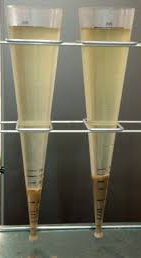
\includegraphics[scale=0.7]{ImhoffCone}\\
%			      		Imhoff Cone\\
%			      		\textit{Note the ml markings at the bottom of the cone}
%			      		
%			      		
%			      	\end{center}
%		      \end{minipage}

 \begin{figure}[h!]
 \centering
        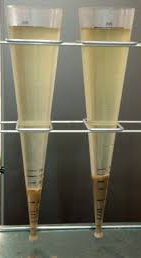
\includegraphics[scale=0.7]{ImhoffCone}
        \caption{Imhoff Cone}
       \textit{Note the ml markings at the bottom of the cone} 
%        \label{fig:sample_figure}
 \end{figure}




			      	\item One factor which affects settleability is the conveyance time of the sewage to the treatment plant. 			
			      	\item The settleable component of the suspended solids will decrease as the sewage becomes more septic due to longer conveyance times.
			\item Influent and effluent total suspended solids are measured to establish the overall treatment and individual process efficiencies.  
			\item Volatile solids measurements before and after biological processes such as secondary treatment and digestion provide information on the process efficiency.\\
		\end{itemize}

\newpage
	\subsubsection{Procedures for Solids Analysis}\index{Procedures for Solids Analysis}
% 		\begin{enumerate}%$$$$$$$$$$$$$$$$$$$$%
% 			\definecolor{shadecolor}{RGB}{220, 220, 220}
% 			\begin{snugshade*}
% 				\item \noindent\textsc{Procedures for Solids Analysis}
% 			\end{snugshade*}		
	\textbf{\textit{Determining wastewater suspended solids - Total (TSS) and Volatile (VSS) concentrations}}

\begin{itemize}
\setlength\itemsep{1em}
					\item A known volume of wastewater sample is filtered through a pre-weighed filter paper
					\item The suspended solids will be retained by the filter
					\item The water with the dissolved solids will pass through the filter
					\item The filter paper with the filter solids is rinsed with distilled water to remove 
					\item The filter paper with the solids is dried in the oven and then weighed
					\item The difference between the weight of the dried filter paper with the solids and the pre-weighed filter paper, measured in mg, will be the suspended solids in: mg per the original quantity of wastewater sample taken.  This value can be converted to give the suspended solids content in mg/l
					\item A filter paper with the dried solids is incinerated in a muffler furnace
					\item The difference in the weight of the solids, before and after incineration is the fixed solids
					\item The difference between the weight of the solids before incineration and the fixed solids is the volatile solids
	\end{itemize}				

\textbf{Total Suspended Solids - TSS}
\vspace{0.4cm}
$TSS \dfrac{mg}{l}=\dfrac{weight \enspace of \enspace solids \enspace \cancel{gms}}{volume \enspace of \enspace sample \enspace \enspace \cancel{ml}}*\dfrac{1000 \enspace \cancel{ml}}{l}*\dfrac{1000 \enspace mg}{\cancel{gms}}$\\
\vspace{0.3cm}
\hspace{1.4cm}$=\dfrac{weight \enspace of \enspace filter \enspace paper  \enspace with \enspace dried  \enspace solids - weight \enspace of \enspace filter \enspace paper}{volume \enspace of \enspace sample \enspace \enspace (ml)}*1,000,000$\\
\vspace{0.4cm}

\vspace{0.4cm}
\textbf{Volatile Suspended Solids - VSS}	
\vspace{0.4cm}

$VSS \dfrac{mg}{l}=\dfrac{weight \enspace of \enspace volatile \enspace solids \enspace \cancel{gms}}{volume \enspace of \enspace sample \enspace \enspace \cancel{ml}}*\dfrac{1000 \enspace \cancel{ml}}{l}*\dfrac{1000 \enspace mg}{\cancel{gms}}$\\
\vspace{0.3cm}
\hspace{1.4cm}$=\dfrac{wt. \enspace of \enspace filter \enspace paper  \enspace with \enspace dried  \enspace solids - wt. \enspace of \enspace filter \enspace paper \enspace incinerated \enspace residue}{volume \enspace of \enspace sample \enspace \enspace (ml)}*1,000,000$\\
\vspace{0.3cm}
$VSS(\%)=\dfrac{weight \enspace (gms) \enspace of \enspace volatile \enspace solids}{100 \enspace gms \enspace total \enspace solids}=\dfrac{gms \enspace volatile \enspace solids}{\cancel{gms \enspace total \enspace solids}}*\dfrac{100 \cancel{\enspace gms \enspace total \enspace solids}}{100 \enspace gms \enspace total \enspace solids}$\\
\vspace{0.3cm}
\hspace{1.5cm}\small{$=\dfrac{wt. \enspace of \enspace filter \enspace paper  \enspace with \enspace dried  \enspace solids - wt. \enspace of \enspace filter \enspace paper \enspace incinerated \enspace residue}{wt. \enspace of \enspace filter \enspace paper  \enspace with \enspace dried  \enspace solids - wt. \enspace of \enspace filter \enspace paper}*100$}\\				

%\textbf{Total solids (TS) and volatile solids (VS)}	
\newpage
	\textbf{\textit{Determining wastewater and sludge total solids - Total (TS) and Volatile (VS) concentrations}}			
\vspace{0.4cm}
\begin{itemize}
\setlength\itemsep{1em}
					\item A certain quantity of wastewater (by volume) or sludge (by weight) is taken in a pre-weighed dish and weighed.  \hl{Note:  the sample is not filtered.}
					\item The dish with the sample is dried in an oven
					\item The difference in the weight of the pre-weighed dish from that of the dish with the dried sample is the total solids
					\item The dried solids are incinerated in a muffler furnace
					\item The difference in the weight of the solids, before and after incineration is the fixed solids
					\item The difference between the fixed solids and the total solids is the volatile solids
					\item Total solids of a sludge sample is reported as a \% of the sludge weight.  A 7\% sludge has 7 lbs of solids for every 100 lbs of sludge.
				\end{itemize}
				
				\hl{For sludge samples, volatile solids is typically reported as the volatile solids fraction in \% of the total solids content of the sludge.  For example, if a 8\% sludge (i.e sludge which has 8\% TS or 80,000mg/l solids), is reported to have 70\% volatile, it means that 70\% of the total solids - 0.7*8\%=5.6\% or 56,000mg/l is the sludge volatile solids content.  \emph{70\% volatile does not meet the sludge has 700,000mg/l volatile solids}}\\	

\vspace{0.4cm}
\textbf{Total Solids - TS}			
\vspace{0.4cm}
$TS(\%)=\dfrac{weight \enspace of \enspace solids \enspace (gms)}{100 \enspace gms \enspace of \enspace sample}=\dfrac{gms \enspace solids}{gms \enspace sample}*100$\\
\vspace{0.3cm}
\hspace{1.2cm}$=\dfrac{weight \enspace of \enspace cruicible \enspace with \enspace dried  \enspace solids - weight \enspace of cruicible}{weight \enspace of \enspace cruicible \enspace with \enspace sample - weight \enspace of cruicible}*100$\\
\vspace{0.4cm}
\textbf{Total Volatile Solids - VS}		
\vspace{0.4cm}
$VS(\%)=\dfrac{weight \enspace of \enspace volatile \enspace solids \enspace (gms)}{100 \enspace gms \enspace of \enspace total \enspace solids}=\dfrac{gms \enspace volatile \enspace solids}{gms \enspace total \enspace solids}*100$\\
\vspace{0.3cm}
\hspace{1.2cm}$=\dfrac{wt. \enspace of \enspace cruicible  \enspace with \enspace dried  \enspace solids - wt. \enspace of \enspace cruicible \enspace incinerated \enspace residue}{wt. \enspace of \enspace cruicible  \enspace with \enspace dried  \enspace solids - wt. \enspace of \enspace cruicible}*100$\\
				\newpage
				\thispagestyle{empty}
				\begin{sidewaysfigure}
					\begin{center}
						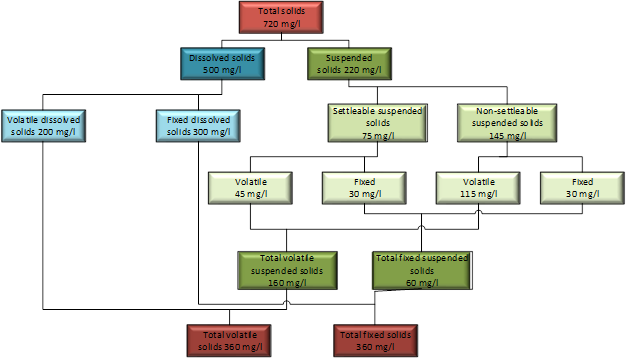
\includegraphics[scale=1.1]{WastewaterSolids}\\
						\caption{Typical Wastewater Solids Concentrations}
					\end{center}
				\end{sidewaysfigure}
\newpage
\thispagestyle{empty}
% \begin{landscape}
% \begin{center}
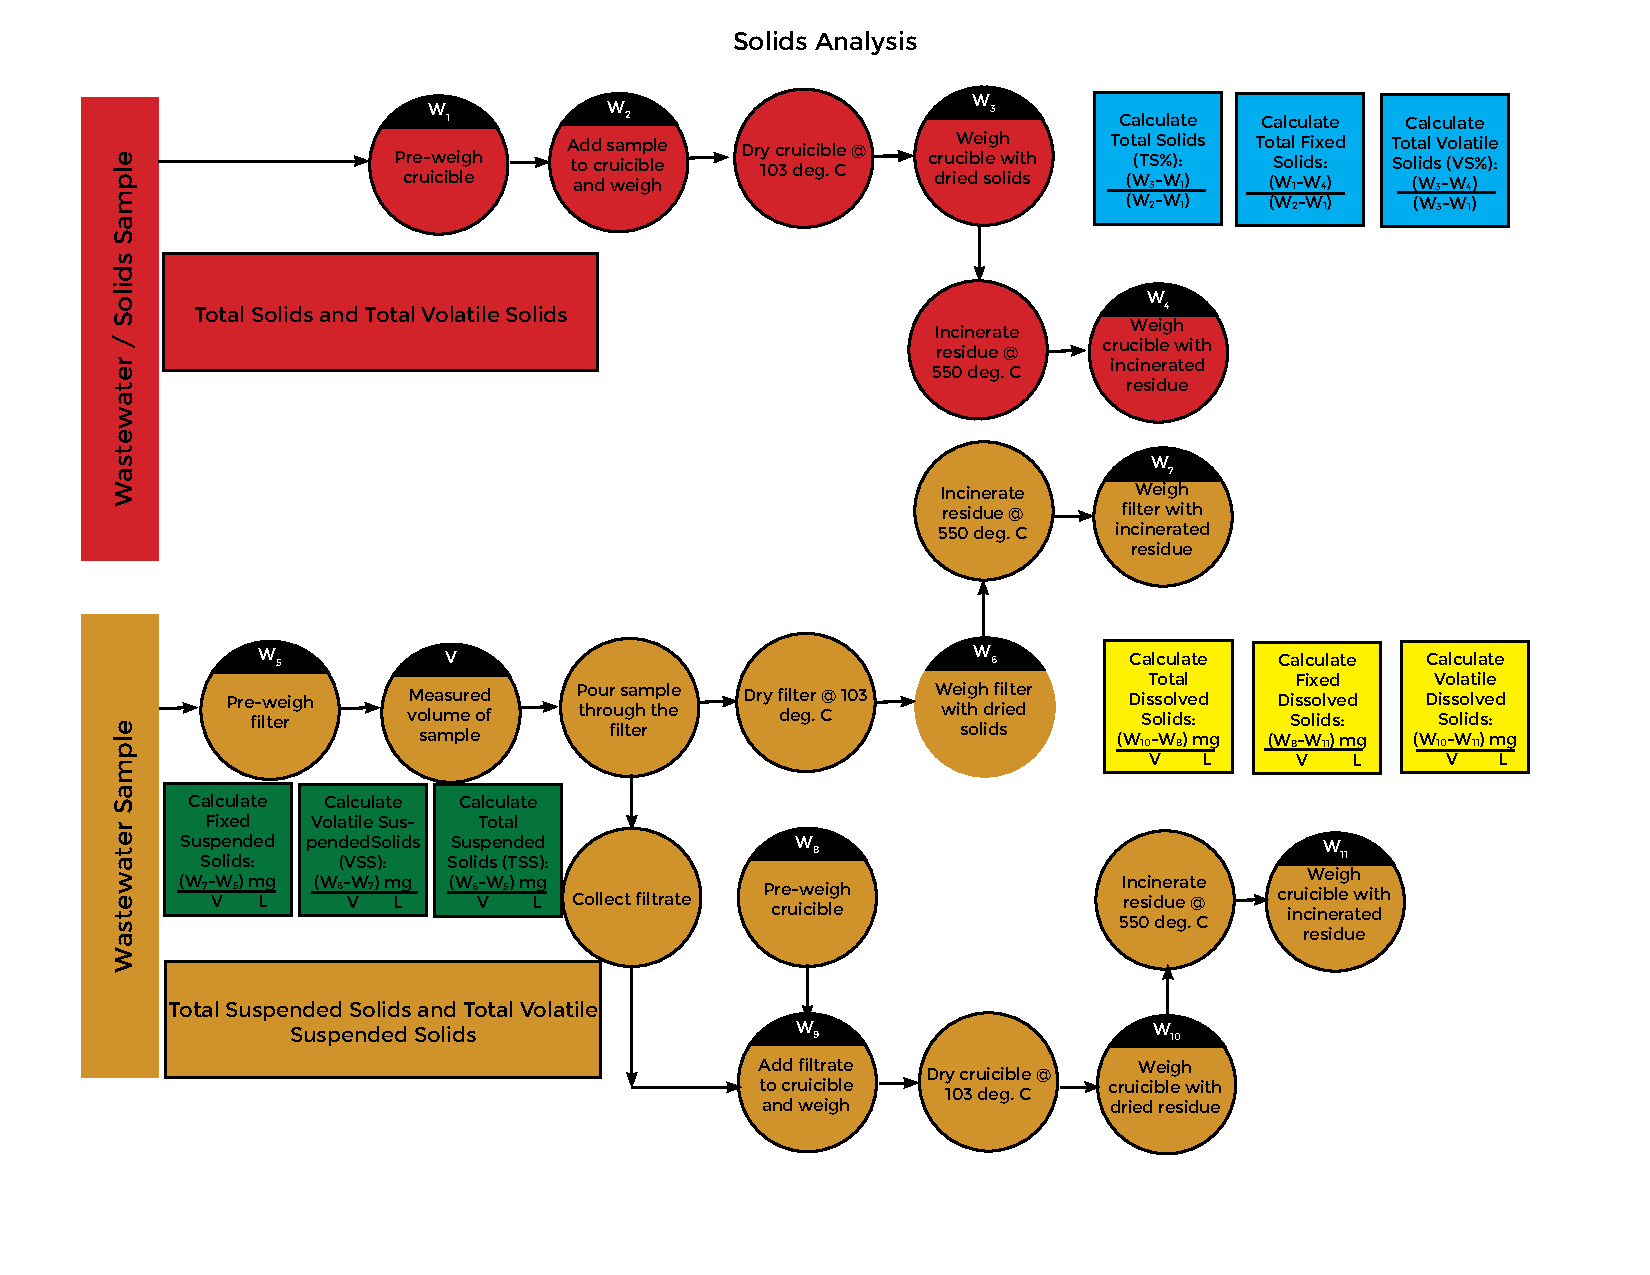
\includepdf[landscape=true]{LaboratorySolidsAnalysis4_01.pdf}
%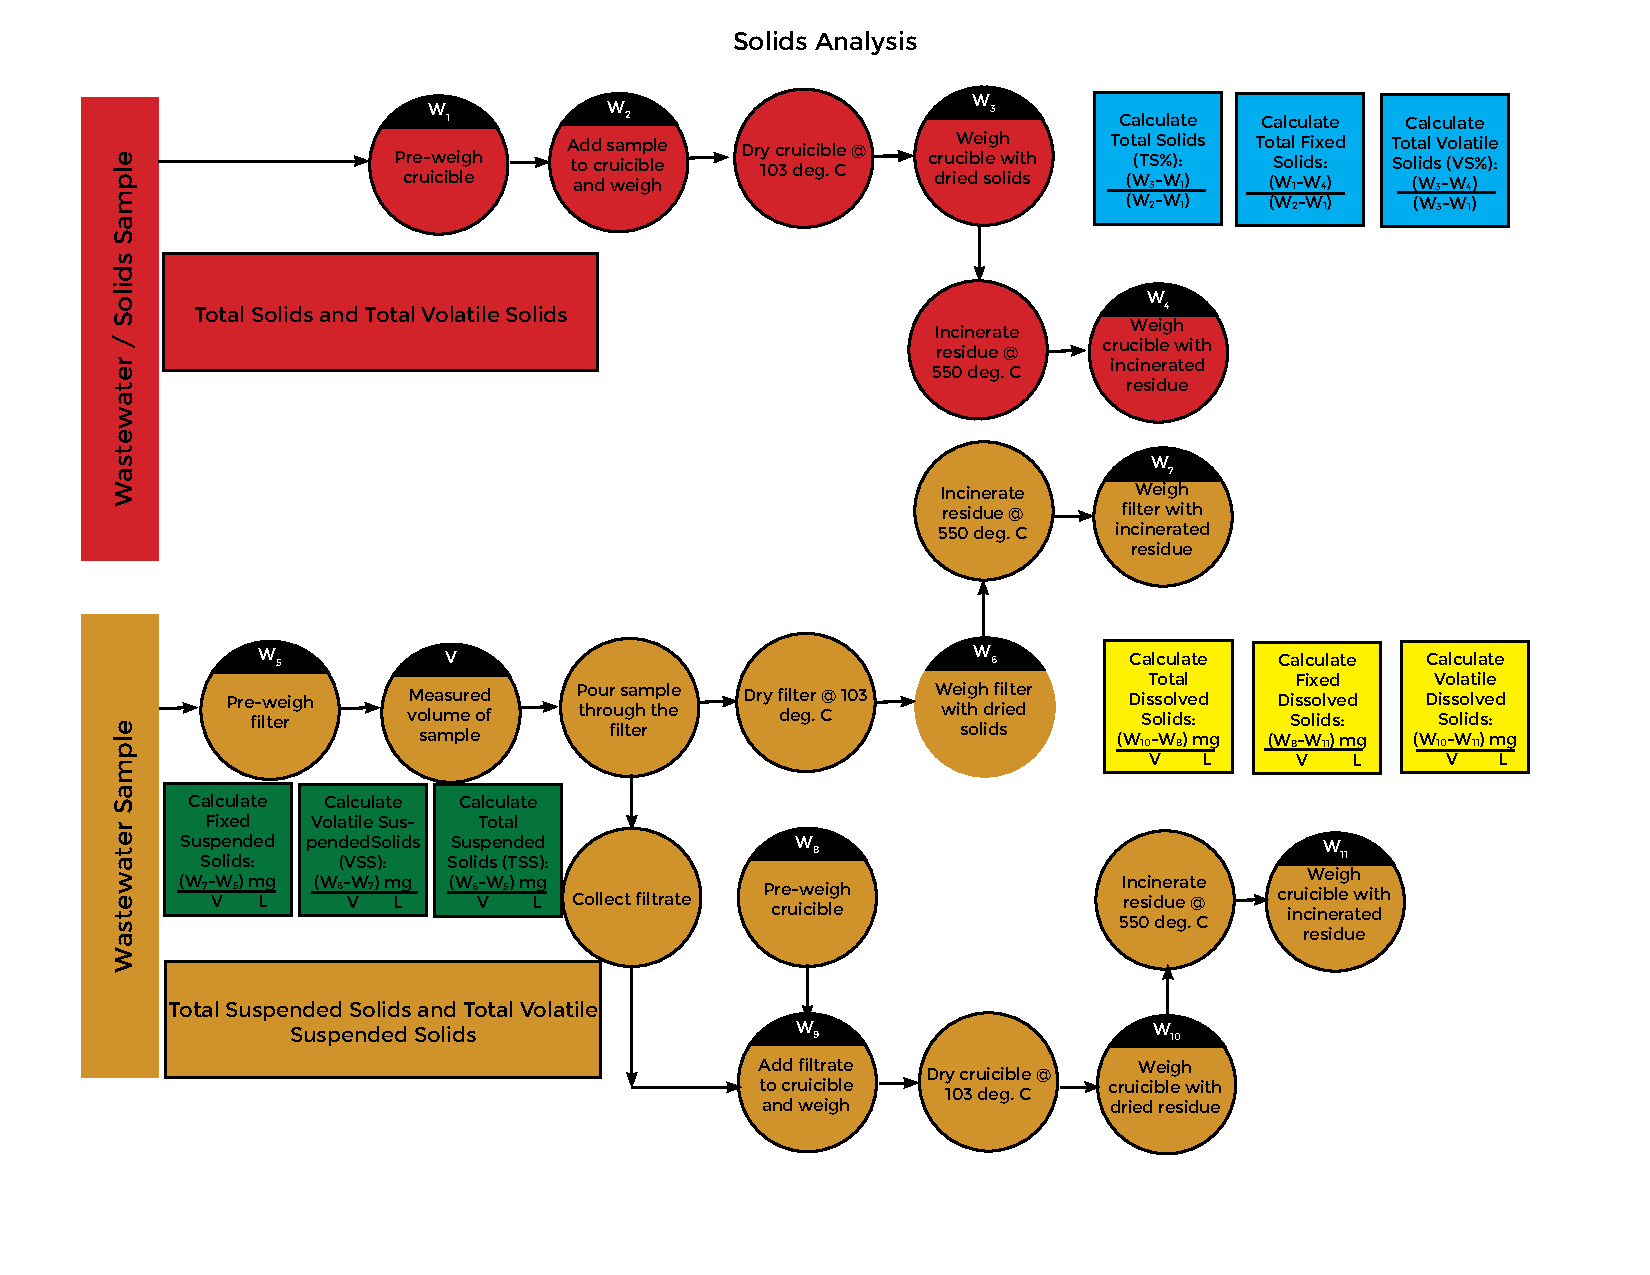
\includegraphics[scale=0.69]{LaboratorySolidsAnalysis4_01.pdf}
% \end{center}
% \end{landscape}
\subsubsection{Sample BOD and solids analysis math problems}\index{Sample BOD and solids analysis math problems}
\begin{enumerate}
\item BOD tests are run on the final effluent from an activated sludge plant with and without the use of a "nitrification inhibitor". Three hundred milliliter bottles (300 ml) are used in these tests. The raw data for these tests are presented below.  What \textbf{percentage of the average total BOD is the average nBOD}?\\
\vspace{0.5cm}
\begin{tabular}{m {4 cm} m {1.5 cm} m  {1.5 cm} m  {1.5 cm} m  {1.5 cm} m {1.5 cm}}
\cline{1-6}
Sample Volume, ml    & 10 & 20 & 30 & 40 & Blank\\
\hline
Initial DO, mg/l 			& 9.0 	& 	8.9 & 8.8  & 9.1 & 9.1\\
Final DO, mg/l 			& 6.9 	& 	4.8 & 2.5 & 1.1 & 9.0
\end{tabular}
\vspace{0.7cm}\\
BOD Test with "inhibitor" added	(cBOD)\\
\vspace{0.5cm}
\begin{tabular}{m {4 cm} m {1.5 cm} m  {1.5 cm} m  {1.5 cm} m  {1.5 cm} m {1.5 cm}}
\cline{1-6}
Sample Volume, ml    & 10 & 20 & 30 & 40 & Blank\\
\hline
Initial DO, mg/l 			& 8.9 	& 	8.9 & 9.0  & 9.0 & 9.1\\
Final DO, mg/l 			& 7.5 	& 	6.2 & 5.0 & 3.3 & 9.0
\end{tabular}
\vspace{0.5cm}\\
Solution:\\
Blanks for both tBOD and cBOD are both <=0.2mg/l - thus sample sets are acceptable\\
\vspace{0.5cm}
\begin{tabular}{m {3 cm} m {2.5 cm} m  {2.5 cm} m  {2.5 cm} m  {2.5 cm} }
\cline{1-5}
Sample Volume, ml    & 10 & 20 & 30 & 40 \\
\hline
tBOD Diff., mg/l    & 2.1 & 4.1 & 6.3 & 8 \\
tBOD, mg/l    & 2.1*300/10 & 4.1*300/20 & 6.3*300/30 & 8.0*300/40\\
    & =63.0 & = 61.5  & = 63.0 & = 60.0 \\
\hline
cBOD Diff., mg/l    & 1.4 & 2.7 & 4.0 & 5.7 \\
cBOD, mg/l    & Reject & 2.7*300/20 & 4.0*300/30 & 5.7*300/40\\
    & Depletion < 2 & = 40.5  & = 40 & = 42.75 \\
\end{tabular}
\vspace{0.5cm}\\

$tBOD (avg) = (63+61.5+63+60)/4=61.9 \hspace{1cm} cBOD (avg) = (40.5+40+42.75)/3=41.1$\\
nBOD = tBOD - cBOD $\implies$ nBOD = 61.9-41.1=20.8 $\implies$ nBOD(\%)=20.8/61.9*100=$\boxed{33.6\%}$
\vspace{0.5cm}
\item Calculate percent total solids and percent volatile solids of a sludge sample given the following data:\\
\begin{tabular}{m {5 cm} m {0.5 cm} m  {3.5 cm}}
Weight of dish &=&  104.55 gms\\
Weight of dish and wet sludge &= & 199.95 gms\\
Weight of dish and dry sludge &= & 108.34 gms\\
Weight of dish and ash &= & 106.37 gms
\end{tabular}\\
\vspace{0.2cm}
Solution:\\
\vspace{0.2cm}
Weight of dish=104.55 gms\\
Weight of dish and wet sludge=199.95 gms\\
Weight of dish and ash = 106.37 gms\\
\vspace{0.2cm}
$ \implies Weight \enspace of \enspace sludge=199.95-104.55=95.40 \enspace gms$\\
$\implies Weight \enspace of \enspace dry \enspace sludge \enspace (solids)=108.34-104.55=3.79 \enspace gms$\\
$\implies Weight \enspace of \enspace volatile \enspace solids=108.34-106.37=1.97 \enspace gms$\\
\vspace{0.2cm}
$Total \enspace solids (TS\%)=\dfrac{gms \enspace solids}{100 \enspace gms \enspace sludge}=\dfrac{3.79}{95.40} \enspace \dfrac{gms \enspace solids}{\cancel{gms \enspace sludge}}*\dfrac{100 \cancel{\enspace gms \enspace sludge}}{100 \enspace gms \enspace sludge}=\boxed{3.97\%}$\\
\vspace{0.2cm}
$Total \enspace volatile \enspace solids (VS\%) =\dfrac{1.97}{3.79} \enspace \dfrac{gms \enspace volatile \enspace solids}{\cancel{gms \enspace total \enspace solids}}*\dfrac{100 \cancel{\enspace gms \enspace total \enspace solids}}{100 \enspace gms \enspace total \enspace solids}=\boxed{52.0\%}$\\


\end{enumerate}
\subsection{Nutrients}\index{Nutrients}	
% 			\begin{snugshade*}
% 				\item \noindent\textsc{Nutrients}
% 			\end{snugshade*}	
			\begin{itemize}
				\item Plant nutrients - nitrogen and phosphorous, present in wastewater effluent discharge, promote growth of plant and algal matter in the receiving waters causing destruction of the normal aquatic life mainly due to oxygen depletion - eutrophication.
				      
				\item Because of the potential impacts of the presence of these nutrients in wastewater effluent on the receiving waters,  limits on the levels of these nutrients is typically stipulated in the treatment plant's wastewater discharge permit.
				      
				\item Typically, conventional secondary treatment processes are designed primarily remove the organics from the wastewater.  Secondary treatment process designed to additionally remove nutrients is deemed as tertiary or advanced treatment is termed as Biological Nutrient Removal (BNR).
			\end{itemize}
	\subsubsection{Nitrogen}\index{Nitrogen}				
% 			\begin{enumerate}%@@@@@@@@@@@@@@@@@@%
% 				\definecolor{shadecolor}{RGB}{220,220,220}
% 				\begin{snugshade*}
% 					\item \noindent\textsc{Nitrogen}%@@@@@@@@@@@@@@@@@@%
% 				\end{snugshade*}

	\textbf{\textit{Forms of nitrogen}}
% 				\begin{itemize}
% 					\item Forms of nitrogen:\\
					      \begin{itemize}
					      	\item About 60\% of nitrogen in wastewater is present as ammonia nitrogen (about 60\%).  The ammonium nitrogen is present either in the form of ammonia (NH$_3$ ) or as ammonium (NH$_4^+$ ) ion.   These two forms can rapidly change from one to the other depending on pH and temperature.  Under low pH (acidic) or neutral conditions – pH less than or equal to 7, ammonia exists mostly as ammonium.  Ammonia becomes the dominant form as the pH increases to 8 and beyond.
					      	\item The other dominant form of nitrogen, about 40\% of the total nitrogen is as organic nitrogen
					      	\item Nitrogen measured as Total Kjeldahl Nitrogen (TKN) which is the sum of the organic nitrogen and the ammonia nitrogen concentrations.  Total inorganic nitrogen is the total concentration of ammonia nitrogen, NO3-, and NO2-.   Table provides the concentrations and forms of nitrogen in wastewater.
					      \end{itemize}
					      \setlength{\arrayrulewidth}{0.7mm}
					      \setlength{\tabcolsep}{8 pt}
					      \renewcommand{\arraystretch}{0.8}
					      \begin{center}
					      \begin{table}[!htbp]
					      	\noindent \begin{tabular}[!htbp]{ |p{6cm}|p{2.0cm}|p{2.5cm}|p{2.cm}|}
					      	\hline
%					      	\multicolumn{4}{|c|}{\textbf{Forms of Nitrogen in Wastewater}} \\
%					      	\hline
					      	%\thead{A Head} & \thead{A Second \\ Head} & \thead{A Third \\ Head} \\
					      	%\hline%
					      	
					      	\hspace{1.8 cm}Forms of Nitrogen & \hspace{0.25 cm} Formula & \hspace{.4 cm} Found in & \hspace{.4 cm} Typical \newline \hspace{.2 cm}Conc.\\
					      	\hline
					      	\small Ammonia/Ammonium & \small NH$_3$/NH$_4^{\enspace +}$ &  \small Influent wastewater & 30-50 mg/l\\
					      	
					      	Total Kjeldahl Nitrogen \newline  \small (Ammonia/Ammonium + Organic Nitrogen) &  \small TKN &  \small Wastewater \newline  \small effluent  & 30-60 mg/l \\
					      	
					      	\small Total Inorganic Nitrogen \newline  \small (Ammonia/Ammonium + Nitrite + Nitrate) & \small TIN &  \small  Wastewater \newline  \small effluent  & 1-40 mg/l \\
					      	
					      	\small Nitrate  & $NO_3^{\enspace -}$ &  \small Nitrified effluent &  \small 1-35 mg/l \\
					      	
					      	\small Nitrate  &  $NO_2^{\enspace -}$ &  \small Partially nitrified effluent &  \small 0.1-2 mg/l \\
					      	
					      	\hline
					      	\end{tabular}
					      	\caption{Forms of Nitrogen}
					      	\end{table}
					      \end{center}
				      
		\subsubsection{Phosphorous}\index{Phosphorous}			
\textbf{\textit{Forms of phosphorous}}
					      \begin{itemize}
					      	\item The principal forms are organically bound phosphorus, polyphosphates, and orthophosphates.
					      	\item Organically bound phosphorus originates from body and food waste and, upon biological decomposition of these solids, is converted to orthophosphates. 
					      	\item Polyphosphates originate from synthetic detergents and are hydrolyzed to orthophosphates. Thus, the principal form of phosphorus in wastewater is assumed to be orthophosphates, although the other forms may exist. Orthophosphates consist of the negative ions PO$_4$$^{3-}$, HPO$_4$$^{2-}$, and H$_2$PO$_4$ $^-$.  These may form chemical combinations with cations (positively charged ions).
					      \end{itemize}

\subsection{Oil and Grease}\index{Oil and Grease}	
			Fats, oil and grease in wastewater originate from homes, food establishments and industries.
			\begin{itemize}
				\item Oil and grease content of wastewater is established in the laboratory by extracting it with a solvent - \textit{n}-hexane.  The concentration of oil and grease is reported in mg/l and typical oil and grease content of wastewater ranges from 80 - 120 mg/l
				\item Presence of excessive oils and grease could potentially impact the secondary treatment process
				\item Oils and grease are removed as floatables in primary treatment and sent with the sludge to the digesters
			\end{itemize}
		



\section{Wastewater Parameters}\index{Wastewater Parameters}			
		Laboratory and field tests are conducted to measure parameters which are critical for monitoring and controlling treatment.  The following are the key parameters that are measured.	
			
\subsection{pH}\index{pH}	
			\hl{pH is a measure of the hydrogen ion (H$^+$) content or the acidity or basicity of a solution.}  pH impacts the chemical and micribiological elements of wastewater treatment processes and thus pH measurement and control is critical.
			\begin{itemize}
				\item Pure water dissociates into equal concentration of hydrogen ions and hydroxide ions:\\ 
				      $H_2O \rightarrow H^+ + OH^-$.
				\item The H$^+$ are responsible for acidic properties and the OH$^-$ ions for the basic properties.  
				\item pH is the inverse of H$^+$ concentration; pH increases when the concentration of H$^+$ decreases relative to the concentration of OH-. 
				\item pH scale ranges from 0 – 14. When the concentration of both H$^+$ and OH$^-$ are equal, as in pure water, it is considered neutral and its pH is 7.0.  \item If the pH of a sample solution is below 7.0, the sample is termed acidic and is alkaline or basic if its pH is above 7.0. 
				\item Each change of 1 pH unit represents a 10 fold change in concentration.  For example, a sample with a pH of 2.0 is 1000 times more acidic than a sample with a pH of 5.0. 
				\item pH is measured by an electrode that is sensitive only to H$^+$ or using a pH strip which is essentially an adsorbent paper which is pre-impregnated with chemicals which change color under different H$^+$ concentrations.
				\item Most organisms involved in biological wastewater treatment processes do well within a a narrow range of pH near neutral (pH of 7).			
			\end{itemize}
			
\subsection{Oxidation Reduction Potential (ORP)}\index{Oxidation Reduction Potential (ORP)}			
			ORP is a measure of the potential of a wastewater to allow for microbiological oxidation and reduction reactions.\\
			An example of wastewater treatment process where microbiological oxidation involved include the activated sludge process.  Whereas, anaerobic digestion is a microbiological reduction based process.
			\begin{itemize}
				\item ORP value is measured in millivolts (mV), using an electrochemical probe
				\item The measured ORP value provides an indication of the potential of oxidation and reduction reactions in that sample.
				\item A higher positive ORP is indicative of oxidation potential of the wastewater whereas a negative ORP value indicates potential for a reduction reaction to occur.
				\item ORP measurements are used for controlling treatment processes including nitrification, odor control and disinfection.  For example, in the disinfection process utilizing chlorine (bleach), ORP measurements provides the strength of the oxidation potential of chlorine present in the wastewater being disinfected.  This measurement is used for precisely controlling the chlorine dosing.  The proper chlorine control results in optimizing chlorine dosing which reduces potential toxicity issues and dechlorination costs.
			\end{itemize}
			Typical ORP applications include the following processes and process elements
			
			
			\setlength{\arrayrulewidth}{0.3mm}
			\setlength{\tabcolsep}{8 pt}
			\renewcommand{\arraystretch}{0.8}
\begin{table}[h!]			
			\begin{center}
				\begin{tabular}{ |p{9.5cm}|p{4.0cm}|}
					\hline
%					\multicolumn{2}{|c|}{\textbf{Typical Wastewater Process ORPs}} \\
%					\hline
					
					\hline
					\small Collections	Sulfide formation                                & \small -50 to -250 mV  \\
					\small Influent wastewater                                          & \small - 200 mV        \\
					\small Activated sludge	cBOD degradation with free molecular oxygen & \small +50 to +250 mV  \\
					\small Biological phosphorous removal                               & \small +25 to +250 mV  \\
					\small Denitrification                                              & \small +50 to -50 mV   \\
					\small Anaerobic Digestion: Acid formation (Acidogenesis)           & \small -100 to -225 mV \\
					\small Anaerobic Digestion: Methane production (Methanogenesis)     & \small -75 to -400 mV  \\
					\hline
				\end{tabular}
				
			\end{center}
			\caption{Typical wastewater process ORPs}
\end{table}			
\subsection{Alkalinity}\index{Alkalinity}	
			\begin{itemize}
				\item \hl{Alkalinity is the ability of a water to neutralize acids.}  
				\item During certain wastewater treatment processes including anaerobic digestion, acids are generated as a result of microbiological activity.  The bacteria and other biological entities which play an active role in wastewater treatment are most effective at a neutral to slightly alkaline pH of 7 to 8.  In order to maintain these optimal pH conditions for biological activity there must be sufficient alkalinity present in the wastewater to neutralize acids generated by the active biomass.
				\item This ability to maintain the proper pH in the wastewater as it undergoes treatment is the reason why alkalinity is so important to the wastewater industry.
				\item The alkalinity is due to the presence of acid neutralizing bases in the water including the hydroxyl (OH$^-$), carbonate (CO$_3$$^-$) and bicarbonate (HCO$_3$$^-$)  ions.  These ions are of mineral origin and are also formed from carbon dioxide which comes from the atmosphere and from the microbial decomposition of organic material.  The resistance to pH change of the water will continue until all the alkalinity contributing ions are neutralized.  
				\item The pH of a water serves as a guide to the types of alkalinity present in the water but is unrelated to the alkalinity content of a water.  Important Note:  Alkalinity is a measure of the ability to neutralize acids whereas a solution is termed alkaline (or basic) if its pH greater than 7. 
				\item Alkalinity is expressed as milligrams per liter of CaCO$_3$
			\end{itemize}
			
\subsection{Dissolved Oxygen}\index{Dissolved Oxygen}	
			\begin{itemize}
				\item Dissolved oxygen (DO) is the concentration of oxygen dissolved in the wastewater sample and is typically measured in the field using a DO probe.  A titration based Winkler Test is used in the laboratory
				\item The \hl{presence of oxygen indicates an aerobic environment} where dissolved, free oxygen is available for aerobic microorganisms to live, BOD removal in the activated sludge process occurs as a result of the activity of aerobic bacteria.  The absence of DO indicates that the environment or condition is either anoxic or anaerobic.  
				\item \hl{In an anoxic environment, free oxygen is not present, but oxygen is available from its combined  forms - nitrate (NO$_3$ $^-$) and sulfate (SO$_4$ $^-$)} for the the consumption of microorganisms.  Example of an anoxic process is denitrification.  In denitrification, the anoxic bacteria in the presence of food (cBOD) consume the combined oxygen in nitrates (NO$_3$ $^-$ ) and convert it to nitrogen gas.
				\item \hl{The complete absence of oxygen including free and combined oxygen is an anaerobic environment.}
				\item Microorganisms are termed as obligate aerobes if they cannot survive without free oxygen.  Facultative aerobes are microorganisms which can survive in both aerobic and anaerobic environments.  
			\end{itemize}
		\section{Laboratory analysis}\index{Laboratory analysis}			
\subsection{Microbiological testing and monitoring}\index{Microbiological testing and monitoring}	
			
			Microbiological testing and monitoring is conducted as part of the wastewater treatment for two main reasons:
			\begin{enumerate}[1.]
				\item Heterotrohic (organisms that consume organic material) microbes are responsible for the biological wastewater treatment processes - secondary treatment process, digestion and nutrient removal; and
				\item Pathogens - agents that cause disease are present in wastewater effluent.
			\end{enumerate}

\begin{itemize}
				
				\item Microbiological testing related to monitoring and troubleshooting biological wastewater treatment\\
				
				Microbes involved in biological wastewater treatment processes include:\\
				\begin{itemize}
					\item Fungi - Filamentous fungi occasionally bloom in activated sludge processes due to low pH or nutrient deficiency and cause problems with the settleability.
					\item Protozoa - Protozoas play a important role in the secondary treatment process.  Common protozoas in the activated sludge process include:
					      \begin{itemize}
					      	\item Amoeba
					      	\item Flagellate
					      	\item Cilliate
					      \end{itemize}
					\item Rotifers
					\item Nematodes
					\item Bacteria - Bacteria is the predominant microorganism responsible for the biological wastewater water treatment.  
				\end{itemize}
				\begin{itemize}
					\item The effectiveness of the biological wastewater treatment processes is primarily due to the presence of a microbial ecosystem with a right balance of populations of different microbial species.
					\item Methods used for monitoring the microbial composition include direct monitoring using a light microscope to see which and how many of the different microbial species are present - typically used for activated sludge process.
					\item Indirect method includes monitoring other parameters such as pH and alkalinity which are influenced by microbiological activity.
					\item The microbial monitoring ensures process stability and helps identify potential process upset conditions caused by changes to the microbial population due to other external factors - toxicty, organic loading, temperature etc.
				\end{itemize}

\item Microbiological testing related to monitoring and controlling pathogens in treated wastewater effluent\\

	
				Pathogens in wastewater belong to the following groups:
				\begin{itemize}
					\item Bacteria:  Although, bacteria is present in large numbers in feces, pathogenic or bacteria are present only because of an infection and this pathogenic bacteria can potentially spread the infection to other healthy individuals.  Disease spread by pathogenic bacteria include diarrhea, cholera and typhoid among many others.
					      
					\item Viruses: A large number of viruses may infect humans and are present in feces.  These include enteroviruses (including polioviruses), hepatitis A virus, reoviruses and diarrhea-causing viruses (especially rotavirus).
					      
					\item Protozoa:  Many species of protozoa can infect humans and cause diarrhoea and dysentery. Girardia which casues diarrheal illness is an example of a protozoan pathogen
					      
					\item Helminths:  These are parasitic worms that can infect humans and are transmitted to others through its eggs or larval forms
					      
				\end{itemize}
				
				\begin{itemize}
					\item As one of the main reasons for treating wastewater is to protect public health, microbiological/pathogen testing of the wastewater effluent and the surface water impacted by the wastewater discharge is conducted to meet the requirements of a wastewater discharge permit, to monitor the pathogen impact of treated wastewater discharge and assess the level of contamination of a public body of water.
					\item The bacteriological tests involves detection and quantification of one or more of the following bacteria:  total coliforms, fecal coliforms, E. Coli, and Enterococcus.  
					      \begin{itemize}
					      	\item The main reason why these bacteria such as coliforms and enterococcus are used \hl{as it is not practical to detect and quantify all pathogens associated with wastewater.}  
					      	\item These selected bacteria originate from feces and indicate fecal contamination and thus serve as an indicator organisms for pathogens of wastewater origin.  
					      	\item Also, they are abundant, potentially less harmful, and easy to detect.  E. coli has been shown to be a better predictor of the potential for impacts to human health and therefore many newer wastewater discharge permits require E. Coli testing in lieu of fecal coliform testing requirements.
					      \end{itemize}
					\item The microbiological test sample is always collected as a grab in a clean, sterile borosilicate glass or plastic bottle containing sodium thiosulfate. 
					      \begin{itemize}
					      	\item Sodium thiosulfate is added to remove residual chlorine which will kill coliforms during transit. 
					      	\item If the sample is not preserved or maintained under proper conditions until the test is conducted in the laboratory, the test would provide erroneous results.
					      	\item Samples must be refrigerated if they cannot be analyzed within 1 hour of collection and must be handled with care to prevent contamination and adverse conditions such as prolonged exposure to direct sunlight.
					      	\item The maximum holding time for state or federal permit reporting purposes is 6 hours. 
					      \end{itemize} 
					\item As it is not possible to exactly quantify the number of bacteria present, a statistical based - \hl{Most Probable Number (MPN)} approach is utilized.  The methods for wastewater bacteriological tests include:  multiple-tube fermentation technique, membrane filtration and quanti-tray testing. 
				\end{itemize}
			\end{itemize}

\subsubsection{Bacteriological Analysis}\index{Bacteriological Analysis}
\begin{itemize}
	\item Involves bacteriological testing of the wastewater effluent and the surface water impacted by the wastewater discharge
	
	\item Conducted in-order to:
		\begin{enumerate}
			\item Meet the requirements of a wastewater discharge permit
			\item Monitor the pathogen impact of treated wastewater discharge
			\item Assess the level of contamination of a public body of water
			\item Bacteriological tests involves detection and quantification of one or more of the following bacteria:  total coliforms, fecal coliforms, \textit{E. Coli}, and \textit{Enterococci}. 
\begin{center}
\tcbox{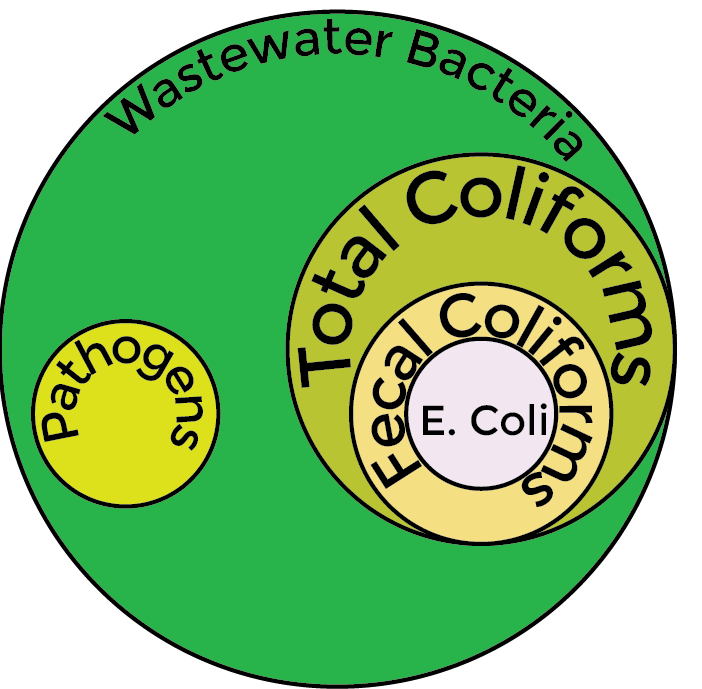
\includegraphics[width=5cm]{LaboratoryWastewaterBacteria}}
Wastewater Bacteria
\end{center}
	
	\item  In wastewater, fecal coliforms originate in the intestines of warm-blooded animals.  Aerobic bacteria including coliforms partake in the metabolization of the organic matter as part of the secondary treatment process
\item Fecal coliforms are seldom pathogenic under normal circumstances and are easily cultured, their presence indicates the potential presence of pathogens

The reason why these bacteria such as coliforms and enterococcus are used:
		\begin{enumerate}
			\item It is not practical to detect and quantify all pathogens associated with wastewater
			\item These bacteria originate from feces and indicate fecal contamination and thus serve as an indicator organisms for pathogens of wastewater origin
			\item They are also:
				\begin{itemize}
					\item abundant
					\item potentially less harmful, and
					\item easy to detect
				\end{itemize}
			\item \textit{E. coli} has been shown to be a better predictor of the potential for impacts to human health and therefore many newer wastewater discharge permits require \textit{E. Coli} testing in lieu of fecal coliform testing requirements.
		\end{enumerate}
		\end{enumerate}

\end{itemize}

\textbf{\textit{Bacteriological Sampling}}

\begin{itemize}
\item Always collected as a grab
\item A clean, sterile borosilicate glass or plastic bottle containing sodium thiosulfate is used. Sodium thiosulfate is added to remove residual chlorine which will kill coliforms during transit. If the sample is not preserved or maintained under proper conditions until the test is conducted in the laboratory, the test would provide erroneous results
\item Samples must be refrigerated if they cannot be analyzed within 1 hour of collection
\item Samples must be handled with care to prevent contamination and adverse conditions such as prolonged exposure to direct sunlight
\item Maximum holding time for state or federal permit reporting purposes is 6 hours
\end{itemize}  


\textbf{\textit{Bacteriological Testing Methods}}
The methods for wastewater bacteriological tests include:  multiple-tube fermentation (MTF) technique, membrane filtration (MF) and quanti-tray testing.  When using the MTF and MF methods, it is not possible to exactly quantify the number of bacteria present, a statistical based - Most Probable Number (MPN) approach is utilized\\

\textbf{The Multiple-Tube Fermentation (MTF) technique}

This involves adding three volumes – 10 ml, 1 ml and 0.1 ml of the sample, each to a set of five tubes containing Lauryl Tryptose broth and an inverted tube (Durham tube), followed by incubating the tubes at  for a specified time.  The Lauryl Tryptose broth produces color and/or turbidity change due to the growth of the target bacteria and the inverted tube collects the gas produced by the bacterial respiration.  At the end of the process, the number of tubes showing bacterial growth are counted for each volume of sample and using this information the concentrations of organisms in the original sample are established using Statistical Tables.  The test is conducted in three parts – presumptive, confirmative and completed.  A schematic of the MTF used for quantifying total coliforms and fecal coliforms is provided below.\\
\newpage
\thispagestyle{empty}
% \begin{landscape}
% \begin{center}
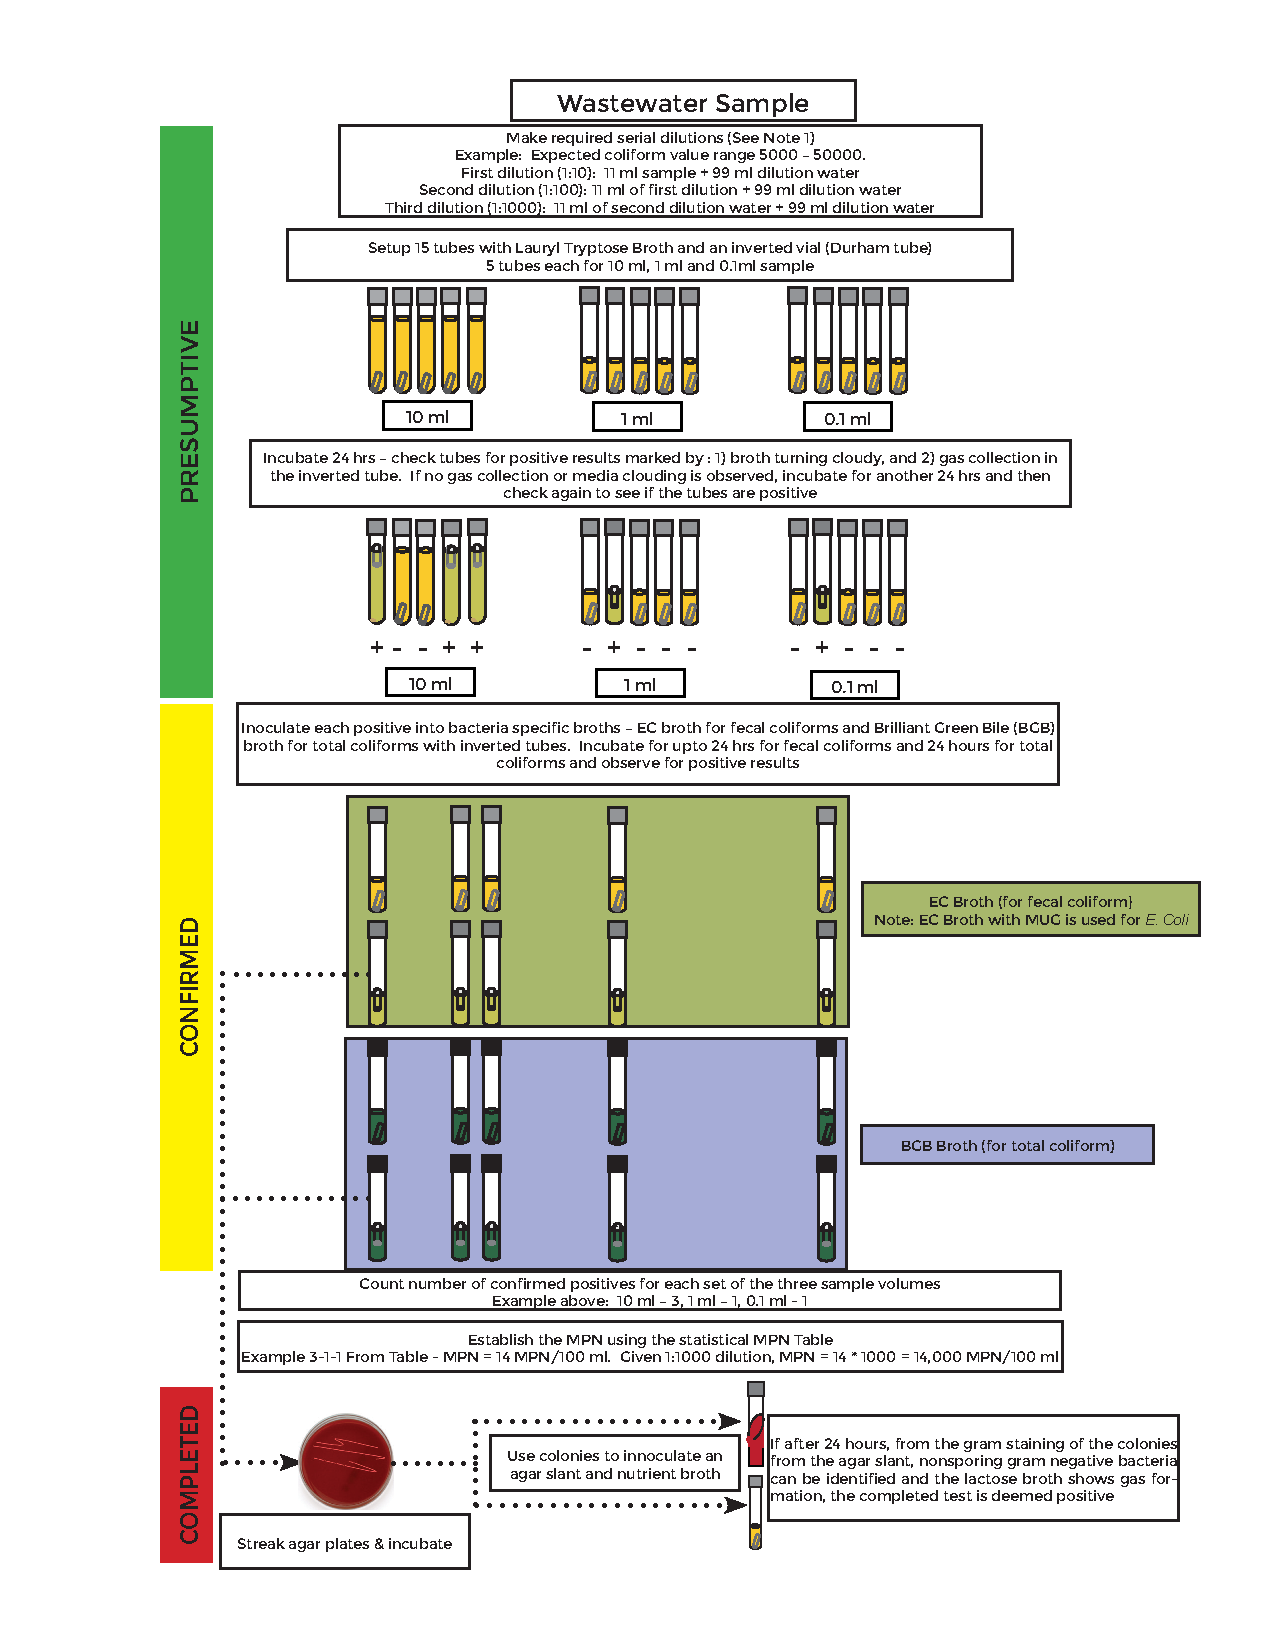
\includepdf[]{MTF.pdf}
%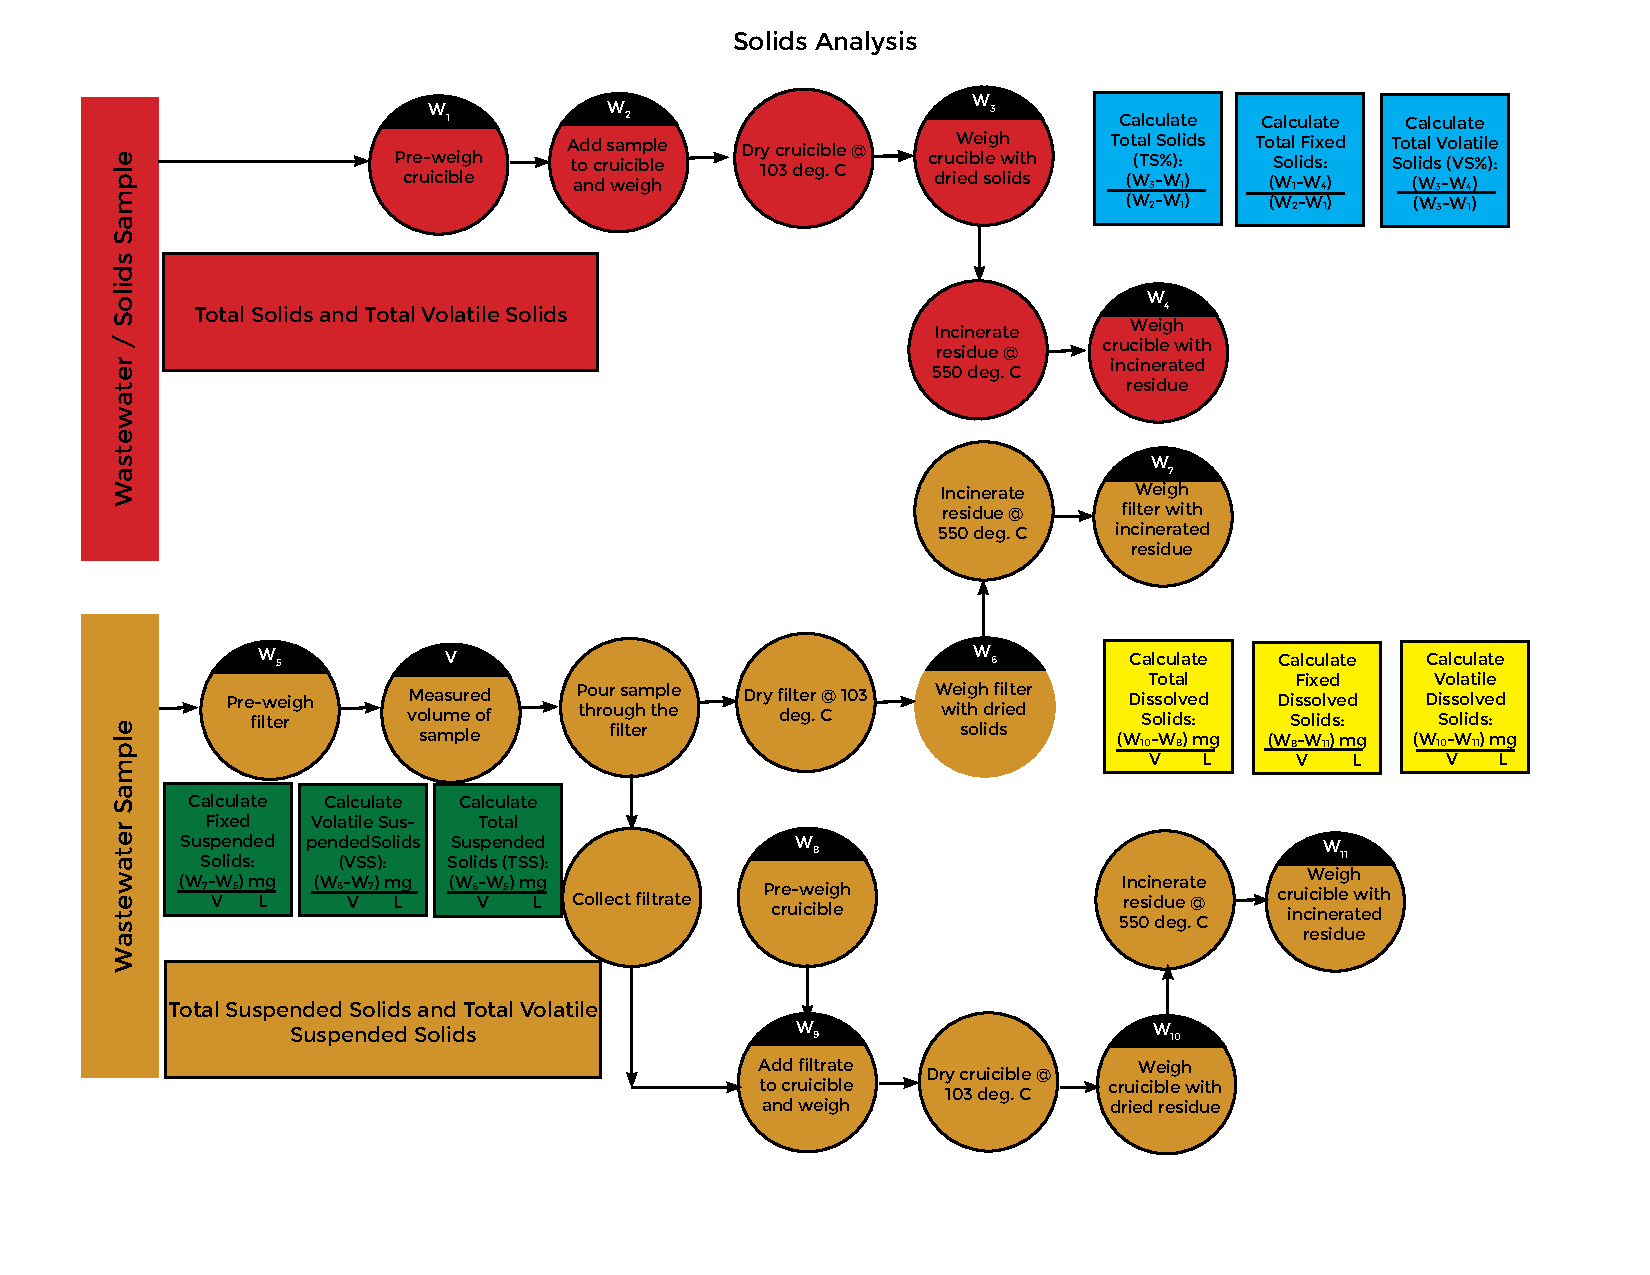
\includegraphics[scale=0.69]{LaboratorySolidsAnalysis4_01.pdf}
% \end{center}
% \end{landscape}
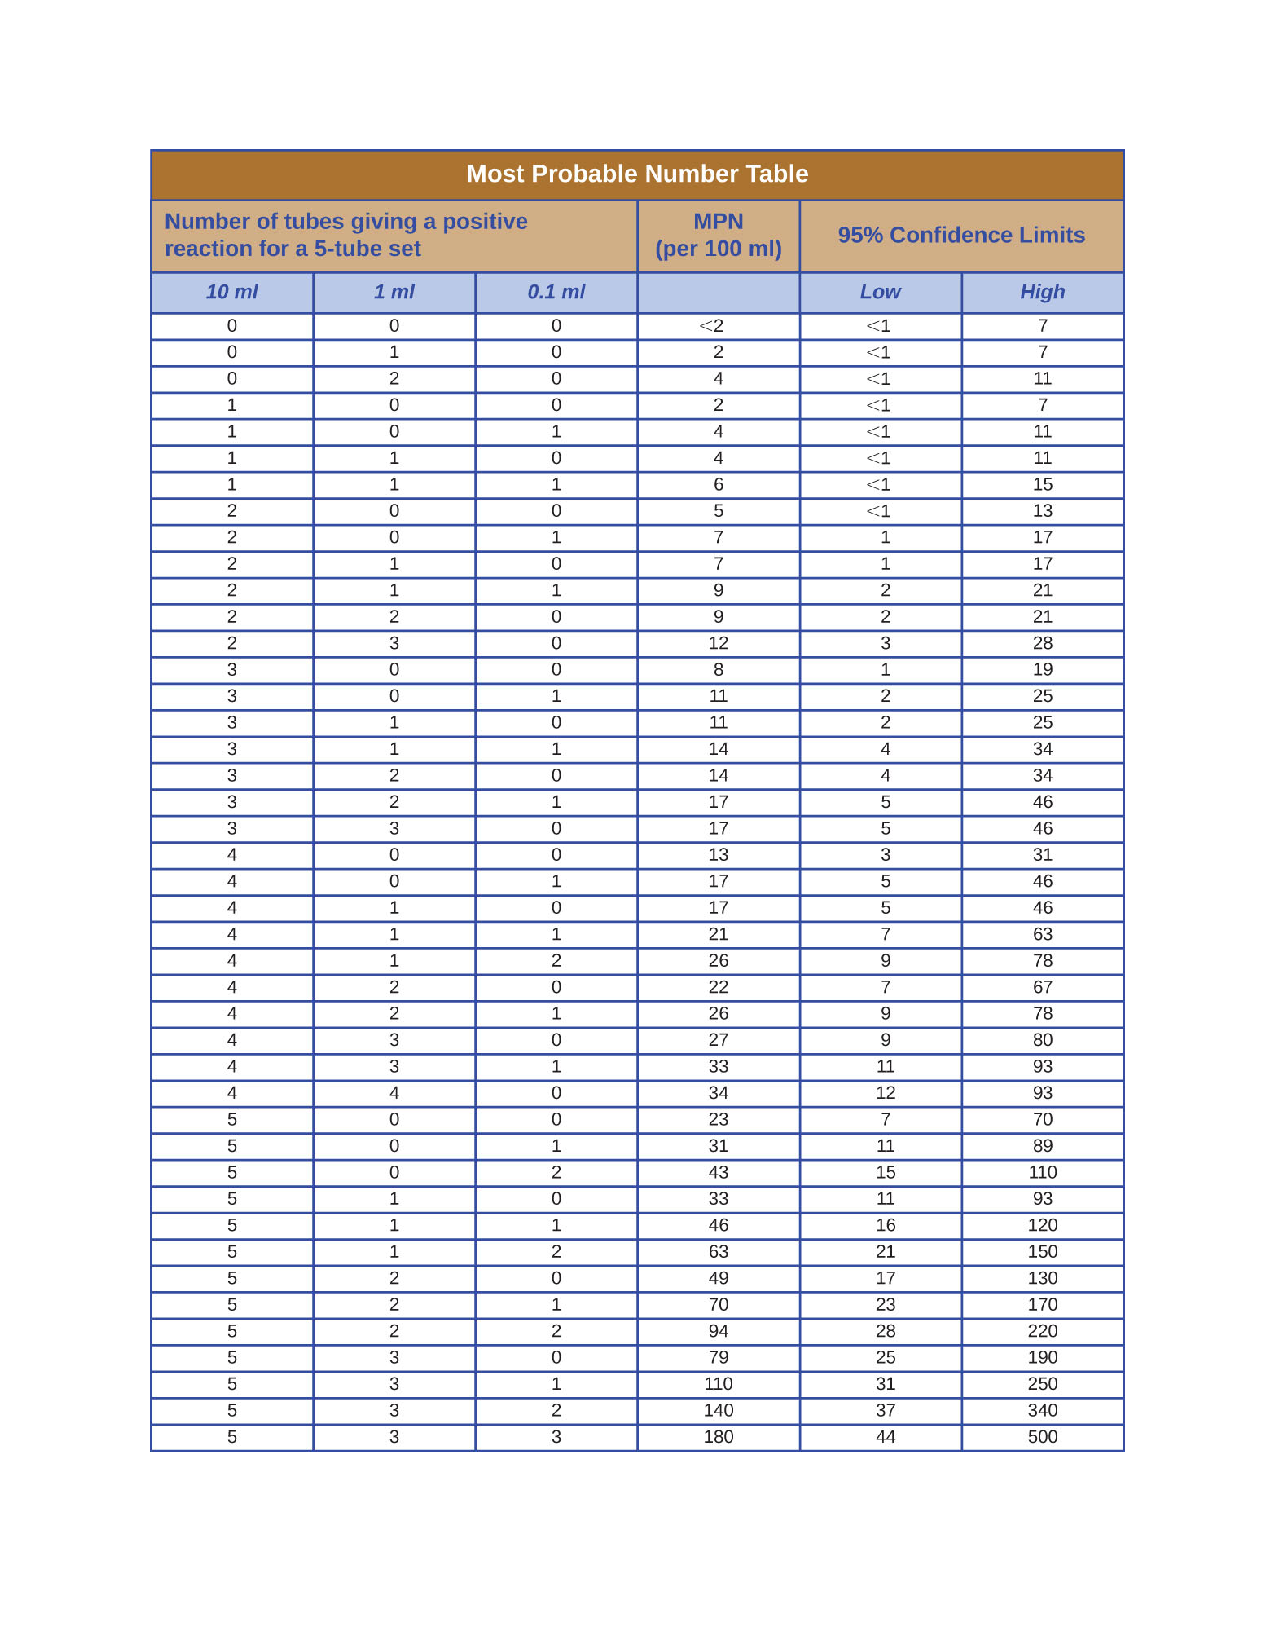
\includepdf[]{MTFTable.pdf}
\newpage

\textbf{The Membrane Filtration (MF) method}
This is a faster way to estimate bacterial populations in water.  In this method, an appropriate sample volume is passed through a membrane filter with a pore size small enough (0.45 micron) to retain the bacteria present. The filter is placed on an absorbent pad (in a petri dish) saturated with a culture medium that is selective for coliform growth. The petri dish containing the filter and pad is incubated, upside down, for 24 hours at the appropriate temperature. After incubation, the colonies that have grown are identified and counted using a low power microscope. A MUG medium is used for E- Coli.  If E. Coli is present, it will make the MUG fluorescent when viewed in UV light. 
\begin{center}
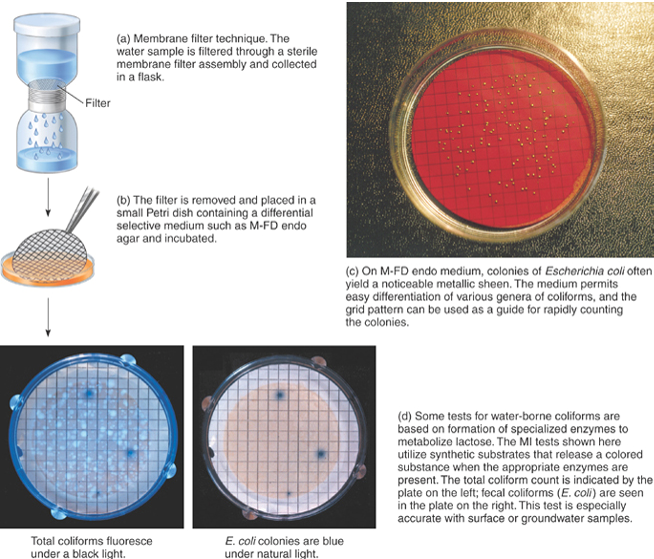
\includegraphics[scale=0.9]{LaboratoryMembraneFiltration}
\end{center}
\pagebreak

\subsubsection{Quanti-trays tests}\index{Quanti-trays tests}

This test used for the detection and quantification of specific microorganisms is being used increasingly mainly because it is a quicker test than the MTF.  Colilert and Enterolert are the quanti tray based tests for E. Coli and Enterococcus.  This method involve the use of specific enzymes and overcomes the drawbacks of the MTF which include false positives and negatives due to the more generic nature of the media used
\begin{center}
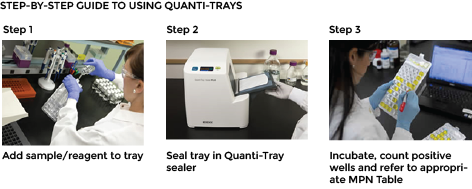
\includegraphics[scale=0.9]{LaboratoryQuantiTray}
\end{center}

\subsection{Specific Gravity}\index{Specific Gravity}				
			\begin{itemize}
				\item Specific gravity is a term to express the weight of a solution with respect to that of water
				\item Water weighs 1 kg/L or 8.34 lbs/gallon or 62.4 lbs/ft$^3$
				\item A solution with a specific gravity of 1.2 will weigh 1.2 times the same volume of water.  1 L of that solution will weigh ( 1.2 kg )/L  or  ( 1.2*8.34=10lbs )/gallon.
				\item Typically wastewater and the associated unthickened sludge, for all practical purposes is assumed to have a specific gravity of 1 - implying 8.34 lbs/gallon.
				\item Specific gravity is typically used for calculations related to chemicals used in wastewater treatment.
			\end{itemize}




\part{Module 2}
\chapterimage{Week2AS.jpg}
\chapter{Activated Sludge}
		\section{Process overview}\index{Process overview}

Activated sludge is a secondary, biological treatment process used for the removal of suspended and dissolved organic matter from the primary treated wastewater.
\begin{itemize}
\item Utilizes an aeration basin/reactor and a secondary clarifier

\item In the presence of oxygen, aerobic bacteria in the aeration basin consume the organic matter (BOD) in wastewater for their growth and reproduction, converting BOD into bacterial cell mass along with metabolic byproducts including carbon dioxide and water

\item The aerobic bacteria is the predominant microbial life form in the aeration basin.  Other higher microbial life forms — mainly protozoa, are present along with some metazoans.

\item The microorganisms along with their metabolic byproducts and residual dead cell mass form a cluster called floc.

\item The wastewater exiting the aeration basin enters a clarifier where the floc settles.  The clear, treated secondary effluent flows out.

\item A portion of the settled activated sludge floc, is returned from the clarifier to the front of the aeration basin to seed the activated sludge treatment of the incoming primary effluent. The recycled floc is called \textbf{Return Activated Sludge (RAS)}.

\item The remaining settled floc from the clarifier is ”wasted” \textemdash transferred for solids treatment (typically using digestion) prior to its ultimate disposal. The wasted floc is called \textbf{Waste Activated Sludge (WAS)}.

\item The color of healthy activated sludge is tan to brown with an earthy/musty odor.

\begin{center}
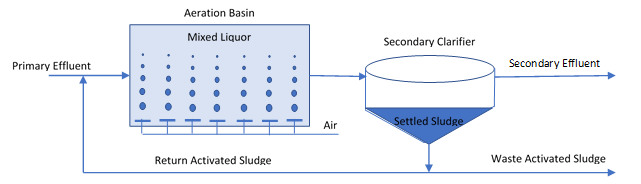
\includegraphics[height=4.5cm]{ASProcess}
\end{center}

\item For activated sludge treatment to be effective, it is critical to establish a healthy microbial population which \hl{converts the BOD} into \hl{easily separable biomass.}
\item If the biomass does not settle well in the clarifier, it will be carried out in the treated secondary effluent producing a poor quality effluent with higher solids and organic content.  \\
\end{itemize}

    \begin{mdframed}[backgroundcolor=blue!20] 
\textbf{Mixed liquor}:
\begin{itemize}
\item Mixed liquor is the mixture of raw and/or treated wastewater with the biomass.
\item Mixed liquor sample is typically taken at the end of the aeration reactor.
\item In the mixed liquor, the suspended solids comprised mostly of biomass with some undegraded and non-degradable material is called \textbf{Mixed liquor suspended solids (MLSS)}.  
\item The volatile fraction of the MLSS is termed \textbf{Mixed Liquor Volatile Solids (MLVSS)}.  \item The MLVSS is the amount of biomass as a percentage of the MLSS.  Generally, the MLVSS is 70 - 80\%, implying that 70-80\% of the MLSS is volatile (organic) solids.
\end{itemize}
    \end{mdframed}


		\section{Process parameters}\index{Process parameters}
\subsection{Dissolved oxygen (DO)}\index{Dissolved oxygen}%$$$$$$$$$$$$$$$$$$$$%
Maintaining adequate \textbf{Dissolved oxygen (DO)} is key to the activated sludge process.  DO is typically maintained between 0.5 to 3.0 mg/l in the aeration reactor.\\
\subsection{pH}\index{pH}%$$$$$$$$$$$$$$$$$$$$%
The microbiological population in the activated sludge is very sensitive to pH and needs to be maintained at neutral - 7 pH.
\subsection{Temperature}\index{Temperature}%$$$$$$$$$$$$$$$$$$$$%
Biological activity is temperature dependent.  Microbial activity approximately doubles for every 10$^o$C rise in temperature.\\
\subsection{Oxygen uptake rate (OUR) and specific oxygen uptake rate (SOUR)}\index{Oxygen uptake rate (OUR) and specific oxygen uptake rate (SOUR)}%$$$$$$$$$$$$$$$$$$$$%

Oxygen Uptake Rate (OUR) involves measurement of the amount of oxygen used up by the microorganisms using a DO probe and is expressed in unit time of mg/L-hr (ppm O$_2$ consumed per hour). By knowing the OUR, we can establish the activity of the microorganisms in the aeration tank and know if they are consuming the oxygen provided for removing organic matter.  \hl{For conventional activated sludge process the typical OUR values range from 10 to 30 mg/L-hr}\\

Specific Oxygen Uptake Rate (SOUR) provides the OUR information based on the concentration of microorganisms present. SOUR is obtained by dividing OUR with MLVSS. The value is indicated and measured in terms of unit of $\dfrac{\dfrac{mg}{l-hr}O_2}{\dfrac{mg}{l}MLVSS}*1000\dfrac{mg}{gm}$.\\ \hl{Optimal range of SOUR is usually between 8 to 20.}\\
If a baseline OUR is established for a system - presence of toxic susbstances in that system can be identified by a drop in OUR. SOUR value above the optimal range indicates an increasing F:M - Higher BOD load with less than adequate microorganisms (represented by MLVSS) indicating a young sludge and the potential for straggler floc.  A lower than optimal SOUR value indicates insufficient food to support the microorganisms indicating an older sludge and the potential for pin floc.

\subsection{Food to Mass ratio (F:M)}\index{Food to Mass Ratio (F:M)}
In order to establish the amount of the MLSS to be maintained in the aeration tank, the parameter \textbf{Food to Mass Ratio (F:M)} is used.  F:M is the ratio of the "food" – the mass of primary effluent BOD entering the aeration basin to the mass of the microorganisms in the aeration basin \textemdash MLVSS.  Common ranges for F:M for a conventional activated sludge plant are from 0.15 to 0.5\\
\subsection{Sludge age}\index{Sludge Age}

\begin{itemize}
\item Sludge age is the average time (days) that a sludge particle (cell) spends in the system.  \item Sludge age dictates the presence and predominance of the different types of organisms and is measured as Mean Cell Retention Time (MCRT) or Solids Retention Time (SRT).\\
\item Sludge age is the average time that a sludge particle (cell) spends in the system
\item Conventional AS process - MCRTs are in the range of 5 to 15 days
\item The desired MCRT for a given plant must be found experimentally
\item \hl{F:M and MCRT are inversely related: that is a long MCRT means a low F:M and a short MCRT means a high F:M} 
\item Both, F:M and MCRT values vary from plant to plant and are established through a trial and error process.
\item The MCRT is calculated as:\\ 
\end{itemize}

\vspace{0.2cm}
$MCRT(days) = $\\
$\frac{Total \enspace MLSS \enspace lbs \enspace in \enspace the \enspace aeration \enspace system \enspace (aeration \enspace tank \enspace + \enspace clarifier)}{Total \enspace amount \enspace in \enspace lbs/day \enspace of \enspace suspended \enspace solids \enspace leaving  \enspace the \enspace system \enspace(Effluent\enspace SS+ WAS \enspace solids)}$\\
\vspace{0.4cm} 
$MCRT (days) = \frac{MLSS \enspace in \enspace aeration \enspace tank \enspace (lbs)+MLSS \enspace in \enspace clarifier \enspace (lbs)}{Effluent \enspace suspended \enspace solids \enspace (lbs/day)+\enspace WAS \enspace SS \enspace (lbs/day)}$

\subsection{Sludge settleability}\index{Sludge settleability}
\vspace{5mm}
\begin{itemize}
\item A settleability test is conducted on the mixed liquor from the aeration reactor to  measure the compaction and settleability characteristics of the secondary solids.
\item In the settleability test, a 1-liter mixed liquor sample is allowed to settle for 30-minutes in a graduated cylinder $-$ settleometer. 
\item The \textbf{Sludge Volume Index (SVI)} of the sludge is calculated using results from the 30-minute settleability test and the MLSS value.
\item SVI is expressed in ml/g and it is essentially the volume (ml) of 1 gram of the MLSS after 30 minutes of settling.
\item SVI (ml/g)= $\frac{Settled \enspace sludge \enspace volume \enspace in \enspace ml/l \enspace after \enspace 30 \enspace min}{MLSS \enspace mg/l}*1000 \frac{mg}{g}$
\item SVI provides a more accurate picture of the sludge settling characteristics than settleability or MLSS alone.
\item 50 to 120 ml/g SVI value is considered optimal.
\item Higher SVI values  indicate sludge that is slow to settle and not compacting well.
\item When SVI values are approaching 200 ml/g, activated sludge process is considered to be "bulking".
\item Regular monitoring of SVI help identify changes occurring in the activated sludge process preventing settling problems before they occur.
\item Like F:M and MCRT, the optimal SVI value for each plant varies and is also established by trial and error.
\end{itemize}


		
				
		\section{Microbiology}\index{Microbiology}
		
Bacteria are fundamental microorganisms in the stabilization of organic wastes and therefore of basic importance in the secondary wastewater treatment process.  

Bacteria (singular, bacterium) are single celled organisms and represent the simplest forms of life.  These organisms utilize soluble food and are capable of self-reproduction.  
Bacteria can be classified in many different ways. 

For wastewater bacteria are classified based on nutritive requirement, bacteria are classified as heterotrophic or autotrophic bacteria, although several species may function both.

\begin{enumerate}[1.]
\item \textbf{Heterotrophic bacteria} use carbon based organic compounds for both energy and food source. A term commonly used instead of heterotroph is “saprophyte” which refers to an organism that lives on dead or decaying organic matter. The heterotrophic bacteria are grouped into three classifications, depending upon their action toward free oxygen.

\begin{enumerate}[a.]
\item
Aerobes : Require free dissolved oxygen to live and multiply. 
\item
Anaerobes : Oxidize organic matter in the complete absence of dissolved oxygen.
\item
Facultative : Use free dissolved oxygen when available but can also respire and multiply in its absence, e.g. Escheichia coli.
\end{enumerate}

\item \textbf{Autotrophic bacteria} use carbon dioxide as a carbon source and oxidize inorganic compounds for energy. Autotrophs of greatest significance in wastewater treatment are the nitrifying and sulfur bacteria.

\begin{enumerate}[a.]
\item Nitrifying bacteria : These bacteria are responsible for the oxidation of ammonia in wastewater to nitrates. 
\item Sulfur bacteria : These bacteria are involved in the formation of sulfuric acid from the dissolved sulfides in the sewer conveyance systems.
\end{enumerate}
\end{enumerate}

The activated sludge is a complex ecosystem of aerobic microorganisms predominantly heterotrophic bacteria along with some autotrophic bacteria and other \hl{trophic organisms} including \hl{protozoas, rotifers and nematodes} which feed on the bacteria and particulate matter.

Protozoa are single-celled microscopic organisms, several hundred times larger than bacteria. \hl{It is the protozoa we observe under a microscope since bacteria are actually too small to see.} There are four types of protozoa commonly found in activated sludge systems. They are identified by their method of movement within the wastewater environment. The four types are:

\begin{tabular}{  m {7 cm}  m {7 cm} } 
\begin{center} 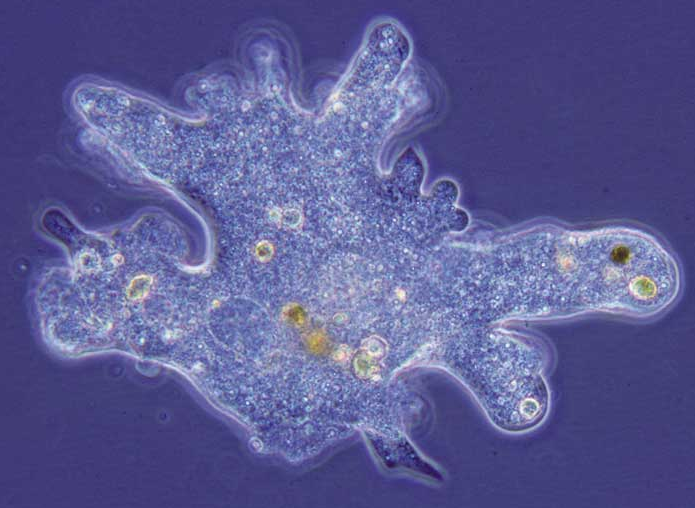
\includegraphics[scale=0.35]{Amoeba} \end{center} & \begin{center}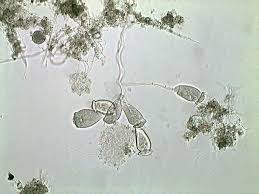
\includegraphics[scale=0.88]{StalkedCilliate} \end{center}\\
\begin{center} \textbf{Amoeba} \end{center} & \begin{center}\textbf{StalkedCilliate} \end{center}\\
\begin{center} 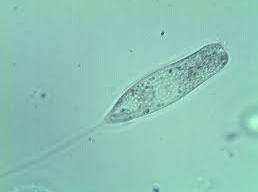
\includegraphics[scale=0.88]{Flagellate} \end{center} & \begin{center}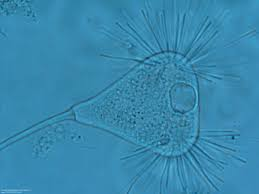
\includegraphics[scale=0.88]{Suctorian} \end{center}\\
\begin{center} \textbf{Flagellate} \end{center} & \begin{center}\textbf{Suctorian} \end{center}\\
\end{tabular}
Other commonly found organisms included the multi-celled organisms - Metazoans such as Rotifers and Nematodes\\
\begin{tabular}{  m {7 cm}  m {7 cm} } 
\begin{center} 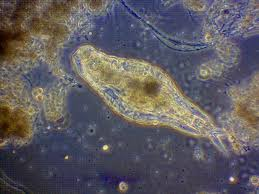
\includegraphics[scale=0.875]{Rotifer} \end{center} & \begin{center}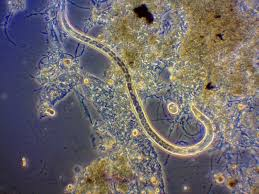
\includegraphics[scale=0.88]{Nematode} \end{center}\\
\begin{center} \textbf{Rotifer} \end{center} & \begin{center}\textbf{Nematode} \end{center}\\
\end{tabular}\\		
				
\begin{itemize}
\item The essence of the activated sludge system is to develop and and maintain a diverse population of microorganisms (activated sludge) that treats wastewater and which can be managed.
\item The activated sludge should be such that it \hl{not only effectively remove the BOD}, but also \hl{produces a floc that settles and compacts well} in the secondary clarifier thereby producing a secondary effluent with a low BOD content.
\item The floc produced has a porous structure and is essentially an aggregate of bacteria and extracelular material including organic polymers - polysaccharides and other substances secreted by the microorganisms, and remnants of dead microorganisms.  
\item Typically, the trophic organisms such as the protozoas and rotifers which feed on the bacteria and other particulates are generally present on the outer surface of the flocs.
\item A good quality activated sludge is brown in color with some froth and a slight musty odor.  
\item The settleability of the sludge is measured as SVI which is the volume of settled sludge in milliliters occupied by 1 gram of dry sludge solids after 30 minutes of settling in a 1,000 mL graduated cylinder or a settleometer.  
\item SVI of a good settling sludge is typically between 50 - 150 ml/g.\\ 
\item MCRT is the key factor which establishes the organism mix in the activated sludge.  
\item As MCRT increases, the size and complexity of the organisms increases.  
\item The types of organisms predominating in the mixed liquor give an indication as to the age of the sludge.
\begin{enumerate}[1.]  
\item At low MCRT of about less than 4 days the simpler protozoas - amoebae and flagellates dominate. 
\item With an increase in MCRT more complex organisms such as the free swimming ciliates and stalked ciliates appear. 
\item At even higher MCRT, metazoans such as the rotifers and nematodes may be found
\end{enumerate}
\end{itemize}
%Following is a chart showing the relative predominance of the trophic microorganisms with respect to the MCRT and its counterpart F:M.

%\begin{center}
%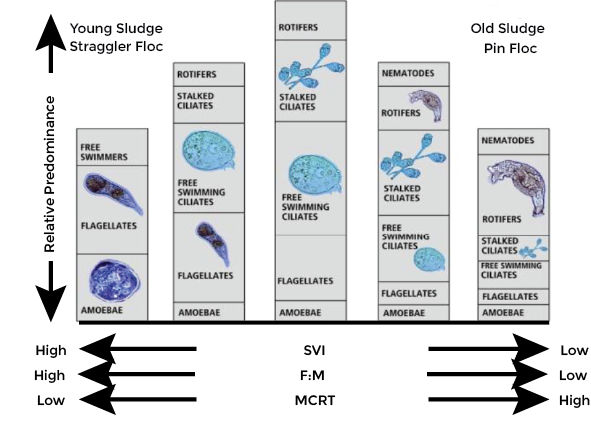
\includegraphics[scale=0.85]{ASRelativePredominance1}
%\end{center}


		\section{Activated sludge process control}\index{Activated sludge process control}	


\begin{itemize}
\item To ensure optimal treatment in the activated sludge process - maximum BOD removal with a well settling mixed liquor, controlling the inventory of solids (biomass) is a key process control parameter.\\
\item New solids (biomass) are produced in the activated sludge reactors due to the consumption of the BOD by the microorganisms.
\item The solids faction of the mixed liquor which separate (settle) in the secondary clarifier are
\begin{itemize}
\item Either returned to the influent end of the activated sludge reactor as Return Activated Sludge (RAS), or
\item removed from the system as Waste Activated Sludge (WAS). 
\end{itemize}
\item Thus, RAS and WAS pumping controls are used for maintaining the desired amount of solids in the system.
\end{itemize}

		\subsection{Controlling waste activated sludge (WAS) pumping rate}\index{Controlling waste activated sludge (WAS) pumping rate}	

For process stability and control the wasting should be continuous and not intermittent and any increase or decrease in wasting should be made gradually, i.e., 20 - 25 percent per day.  One of the following approaches is utilized to establish the WAS flow control 

		\subsubsection{Constant Mean Cell Residence Time (MCRT)}\index{Constant Mean Cell Residence Time (MCRT)}	


Typical MCRT for conventional AS process ranges from 5 to 15 days and 20 to 30 days for extended aeration and for a given plant, the desired MCRT is established based upon operational experience.  WAS flow control can be established to maintain the desired MCRT range for a given plant. 

		\subsubsection{Constant food:mass (F/M)}\index{Constant food:mass (F/M)}	

This parameter is based upon the ratio of food (influent BOD) fed to the microorganisms each day to the mass of microorganisms held under aeration. WAS flow control can be used for controlling the mass of microorganisms in the system to maintain the desired F/M ratio.

		\subsubsection{Constant Mixed Liquor Suspended Solids (MLSS)}\index{Constant Mixed Liquor Suspended Solids (MLSS)}	

A MLSS concentration which provides the best effluent and highest removal efficiencies is selected and WAS flow control is established to maintain the desired MLSS concentration level.  Wasting is increased when the MLSS concentration is higher and decreased or stopped when the MLSS concentration is lower than the desired level.

		\subsection{Controlling the return activated sludge (RAS) rate}\index{Controlling the Return activated sludge (RAS) rate}	

RAS flow rate affects the concentration and the sludge age.  
Return Activated Sludge Control...
To properly operate the activated sludge process,  For conventional activated sludge operations, the RAS flow is generally about 30 to 100\% of the incoming wastewater flow. Changes in the activated sludge quality will require different RAS flow rates due to settling characteristics of the sludge. The following approaches are used to control the RAS flow rate:

		\subsubsection{Constant RAS flow rate control - RAS pumping independent of influent flow}\index{Constant RAS Flow Rate Control - RAS pumping independent of influent flow}	

\begin{itemize}
\item Results in a continuously varying MLSS concentration that will be at a minimum during peak influent flows and a maximum during minimum influent flows. This occurs because the MLSS are flowing into the clarifier at a lower rate during peak flow when being removed at a constant rate. Similarly, at minimum influent flow rates, the MLSS are being returned to the aeration tank at a higher rate than are flowing into the clarifier
\item Maximum solids loading on the clarifier occurs at the initial start of peak flow periods.
\item The clarifier will have has a constantly changing depth of sludge blanket as the MLSS moves from the aeration tank to the clarifier and vice versa. 
\item This RAS control option is especially advantageous for smaller plants as it entails little effort/minimal automation for RAS pumping control.  
\item A disadvantage of using the constant flow approach is that the F/M is constantly changing. The range of F/M fluctuation due to the effect of short term variation in the MLSS (because of hydraulic loading) is generally small enough so that no significant problems arise due to using this approach.
\end{itemize}

		\subsubsection{Constant percentage RAS flow rate control}\index{Constant percentage RAS flow rate control}
\begin{itemize}
\item This approach requires a programmed method for maintaining a constant percentage of the aeration tank influent wastewater flow rate. The program may consist of an automatic flow measurement device, a programmed system, or frequent manual adjustments.
\item The variations in the MLSS concentration due to the diurnal flow profile are reduced and the F/M varies less.
\item The MLSS will remain in the clarifier for shorter time periods, which may reduce the possibility of denitrification in the clarifier.
\item Clarifier is subjected to maximum solids loading when the clarifier contains the maximum amount of sludge. This may result in solids washout with the effluent.\\
\end{itemize}

		\subsubsection{Establishing RAS flow rate based on a solids balance approach}\index{Establishing RAS flow rate based on a solids balance approach}
%Based upon a solids mass balance around the secondary clarifier, formula to calculate the Q\textsubscript{RAS} given Q, MLSS, and SS\textsubscript{RAS}
%
%$$Q\textsubscript{RAS} =(Q * MLSS - \dfrac{Q\textsubscript{WAS} * SS\textsubscript{RAS}}{(SS\textsubscript{RAS} - MLSS)}$$ 
The following equation can be used for controlling RAS flow rate to maintain a target MLSS concentration given the influent flow and the RAS solids content.\\
\vspace{0.3cm}
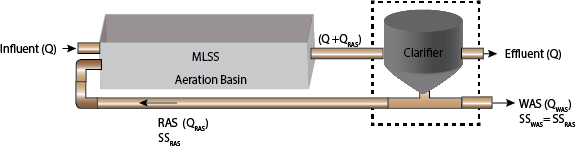
\includegraphics[scale=0.75]{RASQ}\\
Applying a mass balance approach to the secondary clarifier:\\
Mass of solids in = Mass of solids Out\\
$(Q + Q_{RAS})* MLSS = Q_{RAS} *SS_{RAS} + Q_{WAS} *SS_{RAS}$\\
Notes:
\begin{itemize}
\item The solids leaving with the effluent - $Q*SS_{EFF}$ is negligible\\
\item Also, $SS_{WAS}=SS_{RAS}$ \\
\end{itemize}
Rearranging:\\
%$ \implies Q*MLSS + Q_{RAS}*MLSS = Q_{RAS}* SS_{RAS} + Q_{RAS} *SS_{RAS}$\\
%$ \implies Q_{RAS}* SS_{RAS} - Q_{RAS}*MLSS =Q*MLSS - Q_{WAS} *SS_{RAS}$\\
%$ \implies Q_{RAS}*(SS_{RAS} - MLSS) = Q*MLSS - Q_{WAS} * SS_{RAS}$\\  
$ \implies Q_{RAS} = \Bigg(\dfrac{Q*MLSS - Q_{WAS} * SS_{RAS}}{SS_{RAS} - MLSS}\Bigg)$\\
As $Q_{WAS}*SS_{RAS}$ << $Q*MLSS$ and can be neglected\\
Rearranging:\\
$Q_{RAS} = \Bigg(\dfrac{Q*MLSS}{SS_{RAS} - MLSS}\Bigg)$ 
%OR $SS_{RAS} = \Bigg(\dfrac{(Q + Q_{RAS} )MLSS}{Q_{RAS}}\Bigg)$\\


		\section{Process trouble shooting}\index{Process trouble shooting}

The most common activated sludge quality issues include:
\begin{enumerate}[1.]
\item Straggler floc:  This condition shows small, light, and fluffy floc particles with poor settling characteristics. It occurs due to young sludge or low MCRT/MLSS levels and may be related to an inadequate microorganism population or an excessive BOD load (high F:M) which causes a log growth situation. The cells become dispersed rather than flocculated, settleability is poor, and the effluent becomes turbid. In this condition oxygen is used up quickly due to the high metabolism rate, and sludge production is high. One tell-tale sign of this condition is the production of huge amounts of a billowing white foam.

\item Pin floc (Dispersed Growth):  Here flocs - pin floc is seen in the effluent. These are larger dimension spherical particles.  The sludge settles well in the settleability test but the supernatant is cloudy. This floc consist mostly of floc-forming bacteria without a filament backbone.  This condition occurs at starvation condition when all of the influent BOD has been used up (low F:M) and the old sludge age organisms are now in endogenous respiration.

\item Rising sludge: Under this condition, sludge settles well, compacts on the bottom of the clarifier, then starts to rise in clumps and patches to the surface.  Rising sludge is typically evidenced as brown in color.  Rising sludge occurs due to either denitrification or sludge septicity due to an excessive detention time in the clarifier.  

\item Bulking and foaming:  Typical bacteria present in activated sludge include spherical, rod shaped and filamentous.  The presence of filamentous bacteria in activated sludge provide the important structural element for the bacterial floc.  Bulking is indicated by SVI > 150 ml/g. However, certain condition cause an excessive growth of filaments which interferes with the settling (bulking) and cause foaming during aeration.   Identifying which filaments are dominating in the system through a microscopic evaluation will help the operator to understand the condition in the treatment system so that corrective changes can be made.
\end{enumerate}
\begin{center}
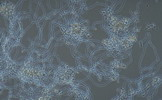
\includegraphics[scale=1.5]{Filaments}\\
Filaments proliferation
\end{center}


\begin{enumerate}[a.]

\item Bulking:  Activated sludge bulking is marked by poor compaction – high SVI\textsubscript{30} and poor solids-liquid separation evidenced by high effluent TSS.  To resolve bulking issue, it is important to find its cause and take remedial actions.  This is accomplished through a microscopic examination to identify the type of the filament to provide a clue on the cause.  Short term remedy to bulking includes Chlorinating – 2-3 mg/l per 1000 lbs MLVSS or use of polymers.

\item Foaming:  Activated sludge foaming is caused mostly by two filaments: Nocardia spp. and Microthrix parvicella (there are other non-filament causes of foaming - including excessive presence of surfactants. Both of these filaments have three causes in combination: (1) high grease and oil; (2) longer sludge age; and (3) low oxygen conditions or septicity.  Foaming if left uncontrolled could potentially pose a permit compliance issue if the foam spills into the effluent.  Additionally, Nocardia from the secondary sludge could cause digester foaming.
\end{enumerate}


\newpage
\thispagestyle{empty}
\begin{landscape}
\begin{table}[ht]
 % title of Table
\centering % used for centering table
\begin{tabular}{ | m {7 cm} | m {4 cm}| m {12 cm}| } 
 \hline
\begin{center}\textbf{Filament Type}  \end{center} & \begin{center} \textbf{Cause} \end{center} & \begin{center} \textbf{Remedy} \end{center}\\
 \hline
 S.natans, Type 1701 and H.hydrossis &  Low D.O. ( For the applied organic loading )&  Low aeration basin DO concentration for the applied F/M leads to filamentous bulking by several filaments.  Typically a minimum DO of 2 mg/l is required for F:M upto 0.5. The condition may also be remedies by raising the MLSS concentration (decreasing the F/M)\\ 
 \hline
 M.parvicella, Nocardia species, Type 0041, Type 0675, Type 1851 and Type 0803 &  Low Organic Loading Rate ( Low F:M )&  Increase the F:M by reducing the MLSS concentration. When reduction in the MLSS concentration may not be feasible due to impact on nitrification, other suitable methods such as the use of a selector may be considered\\
 \hline
 Thiothrix I and II, Beggiatoa species, N. limicola II, Type 021N, Type 0092, Type 0914, Type 0581, Type 0961 and Type 0411 &  Septic Wastes / Sulfides ( High organic acids ) &  Reduce septicity using pre-aeration and through use of chemicals which prevent septicity and reduce sulfides \\
 \hline
 Thiothrix I and II and Type 021N (N defeciency)
N. limicola III (P defeciency)&  Nutrient Deficiency ( N and / or P ) ( Industrial Wastes Only ) & \\
 \hline
Nocardia species, M.parvicella and Type 1863 & High Grease / Oil & \\
 \hline
 Fungi &  Low pH ( Below pH 6.0 ) / Oil  &  The aeration basin pH should be maintained in the range 6.5 to 8.5. Low pH, <6.5, may cause the growth of fungi and fungal bulking. The aeration basin pH can be adjusted using caustic, lime or magnesium hydroxide.\\
 \hline
\end{tabular}
\caption{Troubleshooting Activated sludge filaments}
\end{table}
\end{landscape}
\newpage
		\section{Process modifications}\index{Process modifications}
		\subsection{Conventional activated sludge process}\index{Conventional activated sludge process}

\subsubsection{Process description}\index{Process description}
\noindent The primary effluent (AS influent) - Q, along with the return activated sludge (RAS) - Q$_{RAS}$, are introduced at the head of the aeration tank.  The oxygen demand is the highest at this point and decreases uniformly as the wastewater travels from one end of the tank to the other.\\  


\begin{figure}[h!]
\begin{center}
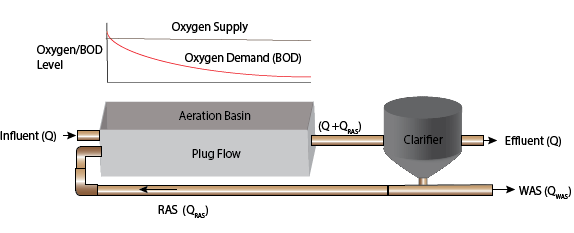
\includegraphics[height=5cm]{ConventionalActivatedSludge}
\caption{Conventional Activated Sludge Process}
\end{center}
\end{figure}


\subsubsection{Process advantages and applications}\index{Process advantages and applications}
The conventional activated sludge process is most suitable for low-strength, domestic wastes with minimal peak load considerations as this process is susceptible to failure from shock loads.  Shock Load is elevated strength (higher BOD and contaminant levels) in wastewater for brief period of time.\\

\textbf{Reasons for modifying the Conventional Activated Sludge Process}\\
Several factors contribute to the need for modifying the Conventional Activated Sludge Process:
\begin{itemize}
\item Unique characteristics of the influent flow which may include - high BOD loads, potential toxic loads, storm flows, loads with high carbonaceous BOD but low nitrogen
\item Space constraints
\item Energy and labor (O\&M) constraints
\item Constraints requiring low solids production
\end{itemize}


		\subsection{Conventional step feed process}\index{Conventional step feed process}



\subsubsection{Process description}\index{Process description}
\noindent In this process modification, the primary effluent is fed to the aeration tank at several different locations within the tank.  The distribution of the influent along the length of the aeration reactor allows for distribution of the load (BOD) over the aeration tank and reduce oxygen sags in the aeration tank.  The return sludge is introduced separately from the primary effluent and in many cases is allowed a short re-aeration period  before mixing with primary effluent.\\

\begin{figure}[bth!]
\begin{center}
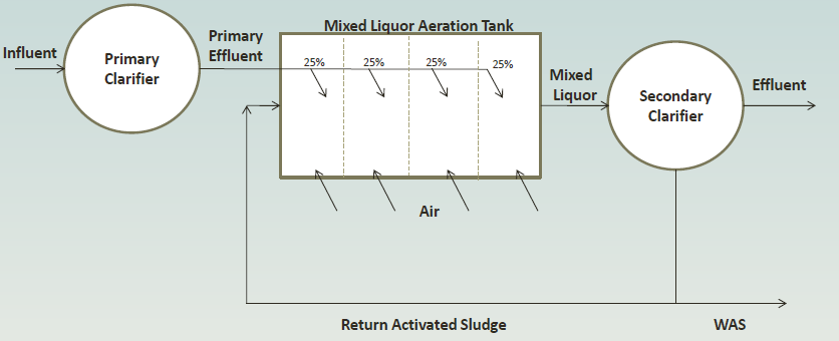
\includegraphics[height=4cm]{StepFeed}\\
\caption{Conventional step feed}
\end{center}
\end{figure}

\subsubsection{Process advantages and applications}\index{Process advantages and applications}
\begin{itemize}
\item Less aeration volume required to treat the same volume of wastewater compared to the conventional aeration.

\item Better control in handling shock loads

\item There is potential for:
\begin{itemize}
\item lower applied solids to the secondary clarifier
\item lower oxygen requirement
\end{itemize}
\item The step-feed process can be utilized on a variable basis using various modes (varying percent of the influent at the feed points) depending on the influent situation and the selection of the proper mode depends on the influent characteristics and the capabilities of the plant to handle the characteristics

\end{itemize}

\begin{figure}[h!]
\begin{center}
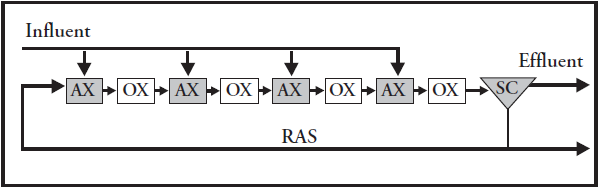
\includegraphics[height=3cm]{StepFeed1}\\
\caption{Step feed modification for Biological Nutrient Removal (BNR)}
\end{center}
\end{figure}

		\subsection{Contact stabilization}\index{Contact stabilization}


\subsubsection{Process description}\index{Process description}
\begin{itemize}
\item This process modification requires two aeration tanks. 
\begin{enumerate}
\item Return Sludge Re-aeration tank:\\
\begin{itemize}
\item This tank is for separate re-aeration of the return activated sludge before it is mixed with the incoming wastewater
\item The residence time in the stabilization tank is typically 4 to 6 hours
\end{itemize}
\item Mixed Liquor Aeration tank (or Contact tank):\\
\begin{itemize}
\item This tank is for mixing of the primary effluent with the re-aerated return activated sludge
\item Here, the organisms quickly take in and store large amounts of food from the primary effluent.
\item The residence time in this tank is approximately 30 to 90 minutes
\end{itemize} 
\end{enumerate}
\end{itemize} 

\begin{figure}[h!]
\begin{center}
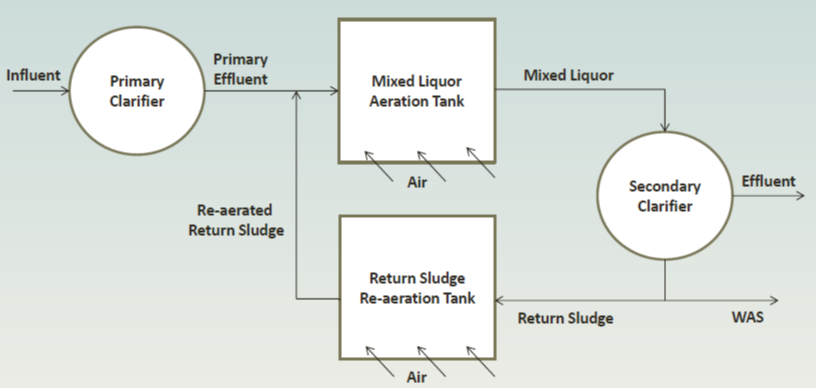
\includegraphics[height=6cm]{ContactStabilization}
\caption{Contact Stabilization}
\end{center}
\end{figure}


\subsubsection{Process advantages and applications}\index{Process advantages and applications}
Because the contact stabilization system has a reservoir of microbes in the re-aeration tank, it is better able to withstand solids washouts that accompany major storms and avoid microbial kill-offs related to short-term toxic dumps

		\subsection{Pure oxygen system}\index{Pure oxygen system}


\subsubsection{Process description}\index{Process description}
\noindent Very similar to conventional activated sludge except that high purity oxygen is supplied to aeration tank (reactor) rather than air and this process treats more wastewater in a smaller space in a shorter period of time.  The Aeration tanks (reactors) are enclosed and sealed to prevent the oxygen from escaping from the tanks.  Pure oxygen from an oxygen generation system or is introduced in the headspace of the reactor.  Mechanical surface aerators agitate the mixed liquor (essentially splash the liquid in the headspace) to dissolve the oxygen into the mixed liquor.  High DO levels are maintained in the aeration tanks (4 mg/l to 15 mg/l).  Roughly 90\%-99\% gaseous O$_2$ goes in and 45-70\% gaseous O$_2$ is ventilated at the effluent end of the reactor.\\

\begin{figure}[h!]
\begin{center}
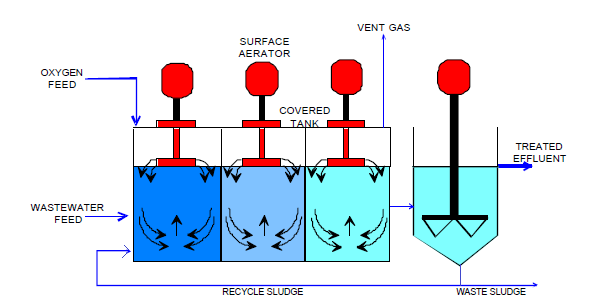
\includegraphics[height=6cm]{PureOx}
\caption{Pure Oxygen System}
\end{center}
\end{figure}

\subsubsection{Process advantages and applications}\index{Process advantages and applications}
\begin{itemize}
\item 
Pure oxygen systems are generally more stable and can treat large volumes of wastewater.  
\item It treats more wastewater in a smaller space in a shorter period of time
\end{itemize}


		\subsection{Sequencing batch reactors}\index{Sequencing batch reactors}



\subsubsection{Process description}\index{Process description}
\noindent Rather than treating a continuous flow through a number of tanks, Sequencing Batch Reactors (SBRs) treat flows in “batches” through a single tank - "reactor" through sequencing stages.  It performs the same treatment steps as a conventional AS plant, but they do it in sequenced stages rather than in a continuous flow stream.  Most commonly preliminary treated wastewater is directly fed to the SBR.

\begin{figure}[h!]
\begin{center}
\tcbox{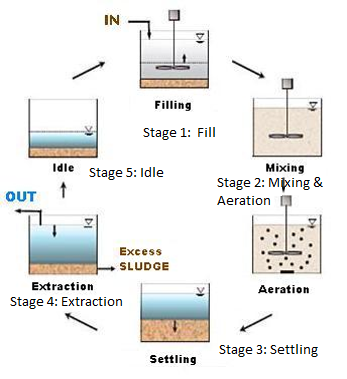
\includegraphics[height=10cm]{SBR}}
\caption{Sequencing Batch Reactor}
\end{center}
\end{figure}


Typically SBR is operated in five stages: 

\begin{enumerate}




\item Filling:  Influent raw wastewater enters the reactor 

\item Mixing \& Aeration:  This stage is where the BOD consumption and biomass production occurs.  Mixing and aeration may be alternated  to accomplish nitrification (during aeration) and denitrification (during mixing - without aeration - anoxic).

\item Settling - This is the clarification stage.  - to allow for the activated sludge floc to settle.

\item Extraction - in this stage the supernatant treated wastewater is removed (for disposal) and part of the settled sludge is wasted.

\item Idle - This stage is essentially to prepare the reactor and the biomass to receive the raw wastewater - Filling stage.  In this stage some aeration/mixing may be provided.  The biomass in the reactor enters the endogenous phase as the food is absent.  The biomass metabolizes the stored food and the organisms feed on one another.
\end{enumerate}


\subsubsection{Process advantages and applications}\index{Process advantages and applications}
\begin{itemize}
\item SBRs are ideal for small facilities as the process can be easily automated

\item SBRs are very stable due to the high sludge ages maintained and the fact that all treatment takes place in a single tank

\item SBR construction is less costly due to the elimination of secondary clarifiers and sometimes digestion facilities (fewer structures in general)
\end{itemize}

		\subsection{Extended aeration}\index{Extended aeration}

\begin{figure}[h!]
\begin{center}
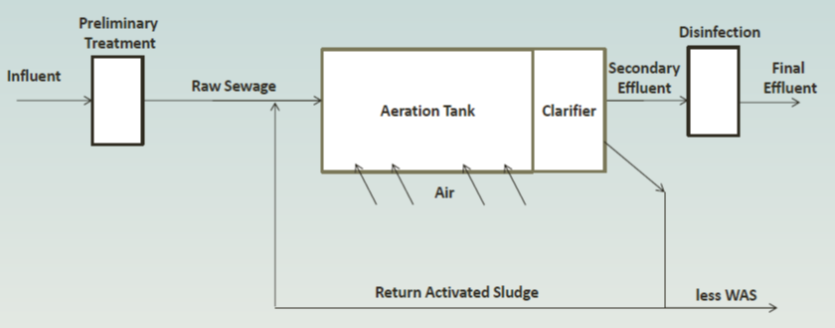
\includegraphics[height=5.5cm]{ExtendedAeration}
\caption{Extended Aeration}
\end{center}
\end{figure}


\subsubsection{Process description}\index{Process description}
\noindent This process typically directs raw sewage flow (without grit/screenings) into the aeration tank where it undergoes treatment for an extended period (usually 8 hours or more – 15 hours typical) followed by clarification.  Mixed liquor concentrations are usually maintained at high concentrations.  Typical F:M ratios are about 0.05 to 0.15 and MCRT of about 30 days.\\

\subsubsection{Process advantages and applications}\index{Process advantages and applications}
\begin{itemize}
\item This process modification is appropriate for small facilities that have light solids loadings – plants typically treating less than 1 MGD – as the aeration tank volume requirement is larger
\item In addition to consuming all the incoming food, the microbes consume all food stored within cells - endogenous respiration, and other dead microbes in the system
\item Extended aeration does not produce as much waste sludge as other process modifications
\item The oxidation ditch is a variation of the extended aeration process.  In the oxidation ditch, the aeration basin is ring or oval shaped.  Aeration rotors or brushes cause the wastewater to flow around the ring and also aerate the wastewater.
\end{itemize}

\begin{figure}[h!]
\begin{center}
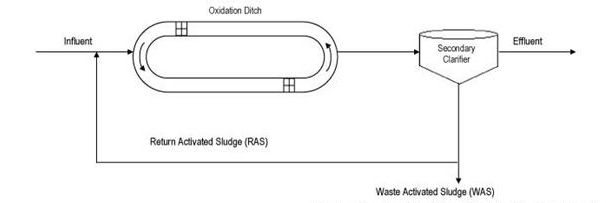
\includegraphics[height=3cm]{OxidationDitch}
\caption{Extended Aeration - Oxidation Ditch}
\end{center}
\end{figure}
\newpage

		\subsection{Krauss process}\index{Krauss process}


\subsubsection{Process description}\index{Process description}
\noindent The process involves use of two aeration tanks.  One aeration tank (Aeration Tank B in the graphic), is for blending return activated sludge (RAS) with anaerobic digester supernatant or sludge and aerating the solution.  The other tank receives primary effluent (Aeration Tank A), return activated sludge, and the aerated mixture of return sludge and digester supernatant/sludge.  Air (oxygen) is added to both aeration tanks.\\

\begin{figure}[h!]
\begin{center}
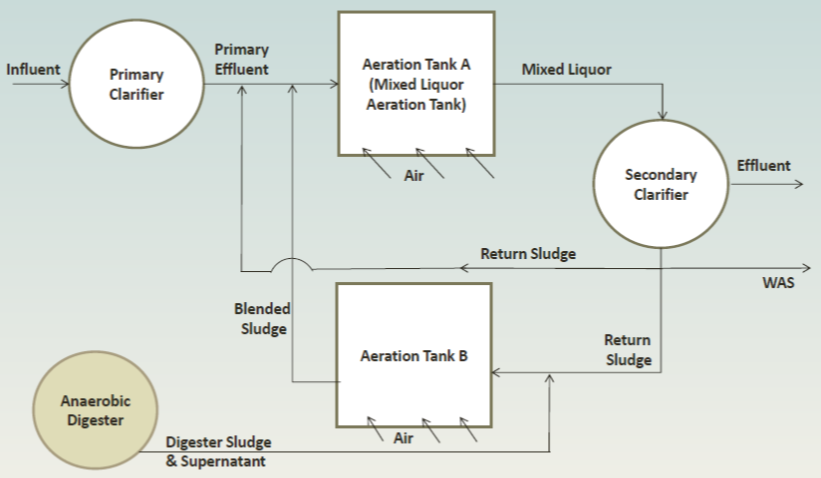
\includegraphics[height=5.5cm]{Kraus}
\caption{Krauss Process}
\end{center}
\end{figure}

\subsubsection{Process advantages and applications}\index{Process advantages and applications}
This process modification is widely used when wastewater contains a high ratio of carbonaceous to nitrogenous material in the wastewater (nitrogen deficient).  This typically occurs when there is significant contribution of wastewater from canneries or dairies.  When the little nitrogen present in the influent wastewater is consumed, further consumption of carbonaceous material ceases.  The digester supernatant or sludge being typically rich in nitrogenous material provides the required nitrogen for the nitrogen deficient process stream.
\newpage
\section{Sample Math Problems}\index{Sample Math Problems}

\begin{enumerate}

\item An activated sludge plant operates well at an F:M ratio of between 0.23 and 0.28.  Calculate the minimum MLSS concentration, given the following:\\
Q = 0.4 MGD\\
Primary influent BOD = 250 mg/l\\
Primary effluent BOD = 128 mg/l\\
Aeration tank vol. = 350,000 gallons\\
Clarifier vol = 250,000 gallons\\
MLSS has 80\% volatile solids\\
\vspace{0.3cm}
Solution:\\
\vspace{0.3cm}
$F:M=\dfrac{(lbs/day) \enspace primary \enspace effluent  \enspace BOD \enspace entering \enspace the  \enspace aeration \enspace tank}{(lbs) \enspace MLVSS \enspace in \enspace the  \enspace aeration \enspace tank}$\\
\vspace{0.3cm}
$\implies F:M \propto \dfrac{1}{MLSS \enspace concentration}$  $\implies$ F:M is inversely proportional to MLSS\\
\vspace{0.3cm}
So to have minimum MLSS conc. F:M needs to be the maximum of the range provided\\
\vspace{0.3cm}
If the MLSS concentration = x:
$ \implies F:M=0.28=\dfrac{0.4*128*8.34}{0.35*x*0.8}\implies x = \boxed{5,446 mg/l \enspace MLSS}$


\newpage

\item Given that an activated sludge plant with an influent flow of 1.2 MGD is operated at an MCRT of 6 days and the parameters below, calculate the WAS flow rate (wasting rate) in gallon per day.
\\
\vspace{0.3cm}
Solution:\\
\vspace{0.3cm}
\renewcommand{\arraystretch}{1.6}
\begin{tabular}{ | m {7 cm} | m {7 cm}| } 
 \hline
Two aeration tanks – 0.5 MG each & Two final clarifiers – 0.25 MG each \\ 
 \hline
 Final effluent $= 20\dfrac{mg}{l}$ & WAS – 7500 ppm\\ 
 \hline
 MLSS –$3600\dfrac{mg}{L}$ & MLSS volatile solids content = 80\%  \\
 \hline
\end{tabular}
\\
\vspace{0.3cm}
$ MCRT \enspace =\dfrac{lbs \enspace MLSS (system)}{\dfrac{lbs}{day} \enspace Effluent_{SS} + \dfrac{lbs}{day} \enspace WAS_{SS}}  $
\\
\vspace{0.3cm}
\noindent \textbf{Step 1:  Calculate the lbs MLSS (system):}\\
\vspace{0.3cm}
\noindent $lbs \enspace MLSS \enspace (system) \enspace =(2*0.5 + 2*0.25)MG * 3,600\dfrac{mg}{L} * 8.34 = 45,036 \enspace lbs$
\\
\vspace{0.3cm}
\noindent \textbf{Step 2:  Calculate the lbs/day Effluent$_{SS}$:}\\
\vspace{0.3cm}
\noindent $\dfrac{lbs}{day} \enspace Effluent_{SS}= 1.2 MG * 20\dfrac{mg}{L} * 8.34 = 200.2lbs$
\\
\vspace{0.3cm}
\noindent \textbf{Step 3:  Plug in the values in the MCRT formula:}\\
\vspace{0.3cm}
\noindent MCRT: $6 \enspace days=\dfrac{45,036}{200.2 \dfrac{lbs}{day}+ \dfrac{lbs}{day}WAS_{SS}}  $
\\
\vspace{0.3cm}
\noindent \textbf{Step 4:  Solving for WAS$_{SS}$:}\\
\vspace{0.3cm}
\noindent $\dfrac{lbs}{day}WAS_{SS} = \dfrac{45,036}{6} - 200.2 = 7,306 \dfrac{lbs}{day}$
\\
\vspace{0.3cm}
\noindent \textbf{Step 5:  Solving for WAS flow using the lbs formula:}\\
\vspace{0.3cm}
\noindent $7,306 \dfrac{lbs}{day} = WAS \enspace Flow \enspace (MGD) * 7,500 * 8.34$\\
\vspace{0.3cm}
\noindent $ \implies WAS \enspace Flow \enspace (MGD)=\dfrac{7,306}{7,500*8.34}=0.116 MGD = \boxed {116,000 \enspace \dfrac{gal}{day}}  $



\end{enumerate}

\part{Module 3}
\chapterimage{NutrientRemovalBW.jpg}
\chapter{Nutrient Removal}

\section{Importance of removing nutrients}\index{Importance of removing nutrients}
\begin{itemize}
\item Plant nutrients - nitrogen and phosphorous, if present in wastewater effluent discharge promote growth of plant and algal matter in the receiving waters causing destruction of the normal aquatic life mainly due to oxygen depletion - eutrophication.

\item Because of the potential impacts of the presence of these nutrients in wastewater effluent on the receiving waters,  limits on the levels of these nutrients is typically stipulated in the treatment plant's wastewater discharge permit.

\item Typically, conventional secondary treatment processes are designed primarily remove the organics from the wastewater.  Secondary treatment process designed to additionally remove nutrients is deemed as tertiary or advanced treatment is termed as Biological Nutrient Removal (BNR).
\end{itemize}

\section{Nitrogen Removal}\index{Nitrogen Removal}

Nitrogen exists in many forms and changes from one form to another in the environment as part of the nitrogen cycle below.

	\begin{itemize}
		\item In raw domestic wastewater, nitrogen exists primarily as organic nitrogen (40\%) and ammonia nitrogen (60\%). 
		\item The sum of organic nitrogen and ammonia nitrogen is referred to as “Total Kjeldahl Nitrogen” (TKN).  
		\item The important forms of nitrogen as part of wastewater treatment are: N$_2$ (Nitrogen Gas), NO$_2^{\enspace -}$ (Nitrite), NO$_3^{\enspace -}$ (Nitrate), NH$_3$ (Ammonia), NH$_4^{\enspace +}$ (Ammonium Ion), and Organic Nitrogen. 
	\end{itemize}
%\floatstyle{boxed} 
%\restylefloat{figure}
\begin{figure}[h]
	\begin{center}
	\includegraphics[scale=0.6]{NitrogenCycle}
	\caption{Nitrogen Cycle}
		\end{center}
\end{figure}

	Typical concentrations of the nitrogen constituents in wastewater are tabulated below.\\

\setlength{\arrayrulewidth}{0.6mm}
\setlength{\tabcolsep}{8 pt}
\renewcommand{\arraystretch}{1.2}
	\begin{center}
	\begin{table}
		%{\rowcolors{3}{green!60!yellow!50}{green!30!yellow!40}
		\begin{tabular}{ |p{6.5cm}|p{2.0cm}|p{2.5cm}|p{2.5cm}|}
			\hline
			\multicolumn{4}{|c|}{\textbf{NITROGEN IN WASTEWATER}} \\
			\hline
			%\thead{A Head} & \thead{A Second \\ Head} & \thead{A Third \\ Head} \\
			%\hline%

			\hspace{1.8 cm}Forms of Nitrogen & \hspace{0.25 cm} Formula & \hspace{.4 cm} Found in & \hspace{.4 cm} Typical \newline \hspace{.2 cm}Concentration\\
			\hline
			\small Ammonia/Ammonium & \small NH$_3$/NH$_4^{\enspace +}$ &  \small Influent wastewater & 30-50 mg/l\\

			\small Total Kjeldahl Nitrogen \newline  \small (Ammonia/Ammonium + Organic Nitrogen) &  \small TKN &  \small Wastewater \newline  \small effluent  & 30-60 mg/l \\

			 \small Total Inorganic Nitrogen \newline  \small (Ammonia/Ammonium + Nitrite + Nitrate) & \small TIN &  \small  Wastewater \newline  \small effluent  & 1-40 mg/l \\

			 \small Nitrate  & $NO_3^{\enspace -}$ &  \small Nitrified effluent &  \small 1-35 mg/l \\

			 \small Nitrate  &  $NO_2^{\enspace -}$ &  \small Partially nitrified effluent &  \small 0.1-2 mg/l \\

			\hline

		\end{tabular}
					\caption{Forms of Nitrogen in Wastewater}
		\end{table}
		
	\end{center}
Ammonia (NH$_3$) and ammonium (NH$_4^+$) are both commonly referred to as “Ammonia-nitrogen (NH$_3$-N)” These two forms of nitrogen can rapidly change from one to the other depending on pH and temperature. The figure below illustrates the relative distribution of ammonia (unionized ammonia) and the ammonium ion (ionized ammonia)in water as a function of pH.\\

\begin{figure}
	\begin{center}
		\includegraphics[scale=.35]{AmmoniaAmmoniumEquilibrium}
			\caption{Ammonia-Ammonium Equilibrium}
	\end{center}
	
	\end{figure}
	\begin{itemize}
		\item In biological treatment processes, the organic nitrogen is quickly changed to ammonia nitrogen by natural processes.
		\item Ammonia-nitrogen is toxic to aquatic life and toxicity is affected by both, temperature and pH of water. 
			\begin{itemize}
				\item Toxicity of ammonia nitrogen increases as temperature increases
				\item Ammonia nitrogen is toxic when present as unionized NH$_3$.  This unionized ammonia NH$_3$ is the predominant form of ammonia nitrogen at higher pH.  The ammonia nitrogen (NH$_3$-N) toxicity is lower when present as  ionized ammonia (NH$_4^+$)
				\item Juvenile fish is more susceptible to ammonia toxicity.  Therefore, ammonia toxicity effects will may be more pronounced during the fish breeding season in spring		
			\end{itemize}
	\end{itemize}
	\vspace{0.3cm}
	
	\subsection{Nitrogen Removal Methods}\index{Nitrogen Removal Methods}
	
		\subsubsection{Nitrification and denitrification}\index{Nitrification and denitrification}

This is the most common ammonia removal process and is accomplished during secondary treatment.  It is a two-step process:
			\begin{enumerate}
				\item \textbf{Nitrification} This involves conversion of ammonia to nitrate
				\item \textbf{Denitrification} This involves conversion of nitrate to gaseous nitrogen which escapes from the waster.
			\end{enumerate}


\noindent\textsc{{Nitrification}}%$$$$$$$$$$$$$$$$$$$$%

			\noindent Nitrification is a two step process:
			
			Step 1:  Nitrosomonas and other similar bacteria oxidizes ammonium to nitrite via hydroxylamine.
			$$2NH_4^{+} + O_2 \rightarrow 2NH_2OH + 2H^{+}$$
			$$NH_4^{+} + 1.5 O_2 \rightarrow NO_2^{\enspace -} + 2H^{+}+ H_2O$$
					 
			Step 2:  Conversion of nitrite to nitrate by nitrobacter and other similar bacteria
			$$NO_2^{\enspace -} + 0.5O_2 \rightarrow NO_3^{\enspace -}$$

			\begin{itemize}
				\item The above two reactions are generally coupled and precede rapidly to the nitrate form; therefore, nitrite levels at any given time are usually below 0.5 mg/L.
				\item Nitrifiers (responsible for the consumption of nBOD) compete with the organotrophs which consume the cBOD in the secondary reactor.  
				\item Nitrification occurs at the tail end of the secondary treatment reactor when the cBOD is low and the organotrophs are not as active
				\item Nitrification occurs 3-4 times slower than carbonaceous oxidation
				\item For nitrosomonas to generate 1 part of new cells it needs 30 parts of ammonium ions and nitrobacter needs 100 parts of nitrite ions to generate 1 part new cells.  Due to the high demand of the nitrogen based ions, the reproductive rates of nitrifiers are very low thus plant upsets can take nitrifiers weeks to recover as opposed to days or hours for carbon bacteria.  
				\item For each 1-gram of NH$_3$-N oxidized to NO$_3$, 0.15 grams of new bacteria cells are formed.  Sludge generation from nitrifiers is minimal in a wastewater treatment plant.
			\end{itemize}
				Controlling Factors for Nitrification:
			\begin{enumerate}
				\item Dissolved oxygen
				\noindent Oxygen levels are critical for nitrification. Higher levels of oxygen are required for nitrification than for carbon removal.  While 1 part of O$_2$ is needed for removing 1 part of cBOD, 4.5 parts of O$_2$ are needed for every part of NH$_4^{\enspace +}N$ (nBOD) to be degraded. In order for nitrification to occur, dissolved oxygen levels of 1.0 to 4.0 mg/L are usually maintained in the aeration tanks.  Maximum nitrification occurs at DO levels of about 3.0 mg/L.  Nitrification will therefore result in significantly higher power cost due to the needs for maintaining the higher oxygen level
				\item Alkalinity and pH

				\noindent \textbf{Nitrification leads to a depletion of alkalinity in the activated sludge mixed liquor.}  Nitrosomonas and Nitrobacter use carbonate as their carbon (food) source and the ammonia is just their energy transfer source.  As the total alkalinity of wastewater is due to the individual contributions of carbonate, bicarbonate and hydroxide ions, consumption of carbonate and bicarbonate ions by the nitrifiers results in the depletion of alkalinity.  Alkalinity provides a buffer for pH change.  If the alkalinity is reduced beyond certain levels, further formation of acidic metabolic byproducts of bacterial activity may lead the pH to decline inhibiting bacterial activity. \textbf{7.14 parts of alkalinity are required for each part of ammonia removed.}    Nitrification rates are rapidly depressed as the pH is reduced below 7.0. pH levels of 7.5 to 8.5 are considered optimal.  That is why alkalinity is extremely critical in nitrification.  An alkalinity of 60 mg/L in the secondary treatment reactor (aeration tank, trickling filter, RBC, etc.) is generally required to ensure adequate buffering
	 			\item MCRT, F/M, or Sludge Age
				\noindent \textbf{For nitrification to occur the activated sludge treatment process needs to be operated at higher MCRT as the reproductive rates of nitrfiers is low.}  An MCRT of greater than 8 days is typically considered essential for nitrification to occur.
				\item Wastewater temperature
				\noindent \textbf{Nitrification is inhibited at lower wastewater temperatures in wastewater treatment plants.} To achieve the same level of nitrification, longer detention time may be needed in the winter versus the summer months since the activity drops significantly.  Lower temperature effects on Nitrification may be partially mitigated by increasing MLVSS and MCRT.  The optimal temperature range for nitrification is between 60$^{\circ}$  to 95$^{\circ}$  degrees F. Below 40$^{\circ}$  nitrification will probably not occur.
	
\floatstyle{boxed} 
\restylefloat{figure}
		\begin{figure}
				\begin{center}
					\includegraphics[scale=0.5]{NitrificationCurve}
								\caption{Weather Effects on MCRT Requirements for Nitrification}
				\end{center}
		\end{figure}
				\item Inhibition to nitrification by toxic compounds
				\noindent Many compounds can be toxic to nitrifiers- Nitrosomonas and Nitrobacter.  These include unionized ammonia, heavy metals, solvents and cyanide.  
			\end{enumerate}
			\newpage
\noindent\textsc{{Denitrification}}%$$$$$$$$$$$$$$$$$$$$%
			\begin{itemize}
				\item Dentrification is a microbiological process in which the nitrate formed during nitrification is reduced by bacteria in anoxic conditions to molecular nitrogen which is insoluble in water and escapes into the atmosphere.
				\item A large percentage of the bacteria in the activated sludge process are capable of denitrification. In the absence of free molecular oxygen – under anoxic conditions, these bacteria present in the activated sludge process utilize the nitrate and nitrite to degrade the cBOD.  
				$$NO_3^- + cBOD   \rightarrow NO_2^- + CO_2 + H_2O$$
				$$NO_2^- + cBOD   \rightarrow N_2 + CO_2 + H_2O$$
				\item Approximately 50\% of the alkalinity lost during nitrification is recovered during denitrification.  
				\item The quantity of cBOD available is critical for denitrification to occur.  Complete denitrification usually occurs at a cBOD to nitrate and nitrite ratio of approximately 3:1. Given the need for the presence of adequate cBOD for the denitrification step, a cBOD supplement (a suitable organic compound - example: alcohol) is utilized in certain configurations.  
				\item If the aeration reactor effluent is nitrified, denitrification can occur in clarifier.  The absence of aeration in the clarifier creates anoxic conditions which makes the condition favorable for denitrification to occur.  Denitrification in the secondary clarifier is not desirable as the nitrogen evolved will cause the sludge settling in the clarifier to rise to the surface.
			\end{itemize}
			\noindent Three of the more common methods to denitrify the nitrified effluent are:\\
			\vspace{0.3cm}
\noindent \textbf{Method 1.}The aeration tank is followed by a denitrifying tank which is not aerated but is supplied with organic substrate (cBOD source) such as methanol or acetic acid.  
				
	\begin{figure}[h]			
				\begin{center}
					\includegraphics[scale=0.8]{Option1}
					\caption{Denitrification Method 1:\\Organic substrate addition}
				\end{center}
	\end{figure}	
\noindent \textbf{Method 2.}The mixed liquor along with RAS is recirculated to an anoxic zone at the inlet of the aeration tank where it is mixed with the influent.  The anoxic zone has mixing provided but no aeration.  The influent flow provides the necessary cBOD for the denitrification process.\\

			\begin{figure}[h]	
				\begin{center}
					\includegraphics[scale=0.8]{Option2}
					\caption{Denitrification Method 2:\\Mixed liquor recirculation}
				\end{center}
					\end{figure}
					\newpage
\noindent \textbf{Method 3.}The aeration tank consists of alternating oxic (aerated) and anoxic zones
				
			\begin{figure}[h]		
				\begin{center}
					\includegraphics[scale=0.8]{Option3}
			\caption{Denitrification Method 3:\\Alternating oxic-anoxic zones}
				\end{center}
				\end{figure}

\subsubsection{Breakpoint chlorination}\index{Breakpoint chlorination}
			\begin{itemize}
				\item Breakpoint chlorination is a means of eliminating ammonia using chlorine
				\item As chlorine is added to water containing ammonia, it converts ammonia into chloramines which in the presence of additional free chlorine forms nitrogen gas which is released to the atmosphere
			\end{itemize} 
Chlorination of a water containing ammonia results in the following:
			\begin{itemize}
				\item an initial increase in combined chlorine residual
				\item followed by a decrease in the combined chlorine residual
				along with ammonia concentrations
				\item followed by an increase in free chlorine residual and near complete removal 					of ammonia as nitrogen gas.\\
				\item Chlorine reacts with ammonia to form chloramines\\
				\begin{enumerate}
					\item First the free chlorine in contact with ammonia forms monochloramine and water
						\begin{itemize}
							\item Monochloramine has disinfection properties\\
							\item Dominates when Cl:N mass ratio is 0 to 5:1\\
							\item The breakpoint curve rises at about 1:1 during monochloramine formation\\
						\end{itemize}
					$NH_3 + HOCl   \rightarrow NH_2Cl (monochloramine) + H2O$\\
					\item Monochloramine reacts further with chlorine to give dichloramine and water\\
					$HOCl + NH_2Cl \rightarrow NHCl_2 + H_2O$\\
					Also, monochloramine auto decomposes into dichloramine\\
					$2NH_2Cl \rightarrow NHCl_2 + NH_3$
						\begin{itemize}
							\item Between dichloramine is formed between 5:1 and 7:1 Cl:N mass ratio
							\item When you are getting significant dichloramine, the breakpoint curve will start dropping
						\end{itemize}
						$NH_2Cl + HOCl  \rightarrow NHCl_2 (dichloramine)$\\
						at pH $>$ 7.5, monochloramine is the dominant chloramine species as pH decreases from 7.5, dichloramine becomes the dominant chloramine species increases in the chlorine to nitrogen dose ratio results in corresponding increases of nitrogen trichloride, but only when the pH is $<$ 7.4\\
					\item Formation of nitrogen trichloride from the reaction of chlorine and dichloramine does not typically occur as it is the favored product at low pH - $<$4\\
					$NHCl_2 + HOCl  \rightarrow NCl_3 (nitrogen trichloride)$\\
					\item Additional $free \enspace chlorine \enspace + chloramines \enspace \rightarrow H^+ + H2O + N_2$
				\end{enumerate}
				\item Chloramines have disinfection properties albeit much lower than free chlorine (~5\% of free available chlorine) but last much longer in the system than free chlorine. 
				\item After the breakpoint, free chlorine residuals develop. Free chlorine residuals usually destroy odors, kill microorganisms and oxidize organic matter.
				\item Breakpoint chlorination is the application of sufficient chlorine beyond the chlorine demand to maintain a free available chlorine residual.\\  Theoretically chlorine requirement = Wt. NH$_3$-N x 7.6\\
				in practice (Margin of safety)     = Wt. NH$_3$-N x 10\\
				\item Thus, breakpoint chlorination is possible if ratio of Cl$_2$ to ammonia exceeds 10:1 then free Cl$_2$ may exist. Cl$_2$ demand will be high because the reaction of free Cl$_2$ with nitrite and other organic compounds. 
				\item Theoretically, while microorganisms are killed as the chlorine demand is being satisfied, disinfection is generally the result of chlorine residual or the amount of chlorine remaining after the chlorine demand has been satisfied.
			\end{itemize}
The following chart is a graphical explaination of the concept of Breakpoint Chlorination\\
			\includegraphics[scale=0.24]{BreakpointChlorination}
			\begin{itemize}
				\item Point A is at the beginning of chlorine application
				\item Between Points A and B, the chlorine dosage produces no residual because of an immediate chlorine demand caused by fast-reacting ions from metal salts and H$_2$S.
				\item Point B is the beginning of the reaction between chlorine and ammonia present
				\item Mono and dichloramines are formed between points B and C
				\item Zone 1 - between points A and C, is the combined zone and has mono and di  chloramines and ammonia.  Mono chloramines is a stable disinfectant while dichloramines is a strong disinfectant but unstable.
				\item After the maximum combined residual is reached (point C), further chlorine doses decrease the residual due to chloramine oxidation to dichloramine, occurring between points C and D.  This is Zone 2 - Breakpoint Zone
				\item Point D represents the breakpoint - the point at which chlorine demand has been satisfied and additional chlorine appears as free residuals
				\item Between points D and E, free available residual chlorine increases in direct proportion to the amount of chlorine applied.  This is Zone 3 which is the free chlorine zone and has hypochlorous acid but no ammonia. \\
			\end{itemize}
			\begin{itemize}
				\item Factors that affect breakpoint chlorination are initial ammonia nitrogen concentration, pH, temperature, and demand exerted by other inorganic and organic species
				\item Weight ratio of chlorine applied to initial ammonia nitrogen must be 8:1 or greater for the breakpoint to be reached. If the weight ratio is less than 8:1, there is insufficient chlorine present to oxidize the chlorinated nitrogen compounds initially formed
				\item When instantaneous chlorine residuals are required, the chlorine needed to provide free available chlorine residuals may be 20 or more times the quantity of ammonia present. Reaction rates are fastest at pH 7-8 and high temperatures
			\end{itemize}


\section{Phosphorous removal}\index{Phosphorous removal}
		\begin{itemize}
		\item Limits related to phosphorous concentrations are commonly found in wastewater treatment facilities' NPDES discharge permits.
		\item Phosphorous removal as part of the treatmnent process accomplishes meeting the NPDES requirement also allows for its recovery for agricultural use.
			\item Phosphorous is very reactive and occurs in nature as phosphate (PO$_4^{\enspace -}$).  
			\item In wastewater phosphorous is present mainly in an inorganic form as orthophosphate (typically about 10 ppm) and as organic phosphate (typically 6 mg/l).
			\item The inorganic phosphate is contributed by detergents and household cleaning products such as soaps
			\item Organic phosphate is contributed by human wastes and food residues as phosphate based molecules play a key role in biological (plant and animals) energy and lifecycles and present in sugars, phospholipids, and nucleotides.  The organic phosphates are decomposed to orthophosphate.
		\end{itemize}
	\vspace{0.3cm}
\subsection{Phosphorous removal methods}\index{Phosphorous removal methods}

\subsubsection{Chemical precipitation method}\index{Chemical precipitation method}

			In the chemical based phosphorous removal method, aluminum and iron salts such as ferric/ferrous chloride and aluminum sulfate react with soluble phosphate to form solid precipitates that are removed by solids separation processes including clarification and filtration. 
			
			Typically, the phosphate precipitant is applied in both the primary clarifier feed and also just before the secondary clarifier.


			\begin{figure}[h]	
				\begin{center}
					\includegraphics[scale=0.55]{PhosphorousChemical}
					\caption{Chemical removal of phosphorous}
				\end{center}
					\end{figure}
\subsubsection{Enhanced biological phosphorus removal (EBPR)}\index{Enhanced biological phosphorus removal (EBPR)}
				\begin{itemize}
					\item For the removal of phosphorous as part of the activated sludge treatment process:\\
					\begin{itemize}
					\item The process is designed to promote the growth of specific aerobic microorganisms generally known as phosphorus accumulating organisms (PAOs) the activated sludge process.  
					\begin{itemize}
					\item Examples of these bacteria in activated sludge: Acinetobacter, Rhodocyclus
					\item These bacteria have the ability to store substantial quantities of intracellular (inside the bacterial cell) phosphorus.
					\item PAOs maybe upto 40\% phosphorous by weight.
					\end{itemize}
					
					\item The process is operated by providing alternating anaerobic and aerobic conditions in the aeration basin of the activated sludge treatment process.
				\end{itemize}
				\end{itemize}
			\textbf{EBPR process description:}
				\begin{itemize}
					\item In the anerobic part of the aeration basin, the aerobic bacteria produce VFAs by breaking down organic matter in the influent wastewater.  Thus, the readily biodegradable material - VFAs, is amply available for the PAOs when in the anaerobic environment.  
						\begin{itemize}
							\item Here the PAOs consume the volatile fatty acids (VFAs) produced by the anaerobic fermentation of the organic matter in the anaerobic zone.  Note: This is a fermentation process not anaerobic digestion (in digestion VFAs are destroyed and converted to methane). 
							\item The VFAs are converted into energy rich, carbon based, storable food source.
							\item The energy for this conversion of the VFA into storable food comes from the breakdown of the PAOs polyphosphate reserves.
							\item Ortho phosphate is released during this phase.  
							\item After exposure to enough VFA, the PAOs energy reserves will be depleted and become stressed.  
						\end{itemize}
					\item In the following aerobic phase of the process the PAOs multiply and take up phosphate to replenish the supplies depleted in the anaerobic phase.  
						\begin{itemize}
							\item By oxidizing the carbon reserves built up in the anaerobic phase, PAOs are able to store more phosphate under aerobic conditions than was released under anaerobic conditions because considerably more energy is produced by aerobic oxidation of the stored carbon compounds than was used to store them under anaerobic conditions.
						\end{itemize}
				\end{itemize} 
Eventhough the EPBR requires only a good aeration, its success in removing phosphorous is dependent on the presence of adequate quantities of readily degradable organic material in the secondary influent.


\chapterimage{SolidsTreatmentOverviewBW.jpg}
\chapter{Solids Treatment Overview}
\section{Why do we need to treat wastewater solids?}\index{Why do we need to treat wastewater solids?}

\begin{itemize}
\item Sludge is generated from the wastewater treatment processes -  settled solids and scum from primary and secondary treatment processes
\item This sludge contain organic compounds and also elements that are beneficial plant nutrients
\item However, the organic solids in the sludge are not stable (i.e. they will decay) and include pathogens.  \item Prior to disposal, sludge has to be treated – stabilized, so that its disposal or reuse does not pose a threat to public health.
\item Sludge treatment is very critical as it is an expensive process and sludge disposal is subject to strict regulatory requirement.
\item Even solids are only a small component of wastewater, the solids treatment and disposal account for a very substantial portion of wastewater treatment costs.  Typically 40 to 60\% of total wastewater treatment operations cost is attributable to sludge treatment and disposal.
\end{itemize}

\textbf{NOTE: Solids removed during Preliminary Treatment, from barscreens and grit chambers are typically not treated as part of the solids treatment process.  These solids are disposed off at a landfill}

\vspace{0.5cm}
\textbf{Typical solids treatment is comprised of the following three sequential steps:
\begin{enumerate}
\item Sludge thickening
\item Sludge stabilization
\item Sludge dewatering
\end{enumerate}}
\vspace{0.5cm}
\section{Sludge thickening}\index{Sludge thickening}
Sludge thickening involves the removal of excess water from the primary and secondary sludge increasing the solids content of the sludge and reducing the volume of sludge to be treated in the sludge stabilization process.
Sludge thickening reduces the volume of sludge that need to be handled in the sludge stabilization step thereby reducing treatment cost.  
\begin{itemize}
\item There is an upper limit of the solids concentration that can be effectively treated (stabilized) as increasing the solids concentration reduces its ability to be mixed and pumped easily.  Typically the sludge thickening process produces sludge with a solids content of less than 10\%.\\
\end{itemize}
Benefits of thickening to the sludge stabilization process include:
\begin{itemize}
\item Improved performance due to a lower volume of sludge
\item Cost savings in the construction of new facilities
\item Reduction in energy requirements as less water has to be heated
\end{itemize}
Typical methods used for sludge thickening include:
\begin{enumerate}
\item Gravity thickener - more suitable for primary sludge
\item Dissolved air floatation thickener - more suitable for lighter, fluffier floc such as the secondary sludge.
\end{enumerate}
\section{Sludge Stabilization}\index{Sludge Stabilization}
\textbf{}\\
Sludge stabilization process produces solids that are deemed safe for eventual disposal.  Federal Part 503 rule establishes requirements for the final use or disposal of sewage sludge.  The solids disposal methods may include: land application, as a crop/vegetation fertilizer, placed on a surface disposal site for final disposal and fired in an incinerator.\\
\textbf{Biosolids is the term used for stabilized sludge which meets regulatory standards for beneficial reuse}\\  

Sludge stabilization process results in the following:
\begin{enumerate}
\item Reduction in amount of solids
\item Pathogen reduction
\item Odor reduction
\item Reduction in vector attraction
\end{enumerate}
The main processes involved in sludge stabilization include:
\begin{itemize}
\item Digestion - Aerobic or anaerobic
\item Lime or alkaline stabilization
\item Composting
\item Long term storage in lagoons
\item Thermal processes
\item Incineration
\end{itemize}

\section{Sludge Dewatering}\index{Sludge Dewatering}
Solids stabilized using digestion process has only a small percentage by weight of solids -less than 5\%.  It therefore becomes necessary to dewater the stabilized sludge prior to hauling off-site for final disposal.  Like thickening, the dewatering process does not treat the sludge.  It increases the solids content to between 15 to 30 percent and the higher solids content of the stabilized sludge makes it easier to handle and reduces costs associated with elements related to accomplishing the end objectives with the sludge – land application, composting, drying, incineration or landfill.\\
Dewatering involves conditioning the sludge with a polymer and subjecting it to a physical process which include:
\begin{enumerate}
\item Belt Filter Press 
\item Centrifuge
\end{enumerate}

\part{Module 4}
\chapterimage{BiosolidsRegulations.jpg} % Chapter heading image

\chapter{Biosolids Regulations}

\section{Biosolids Definition}\index{Biosolids Definition}

		\begin{itemize}
			\item Biosolids are treated solids produced as part of wastewater treatment
			\item Biosolids can be disposed or recycled beneficially
			\item Biosolids must meet standards established under Title 40 of the Code of Federal Regulations (CFR), Part 503.  
			\item Grit and screenings are not considered as biosolids
		\end{itemize}
	
\section{Biosolids Use/Disposal Methods}\index{Biosolids Use/Disposal Methods}
	
			\begin{enumerate}[1.]
				\item Land application
					\begin{itemize}
						\item This is the most commonly used biosolids management method and is referred as a "recycling" option.
						\item This uses the organic and/or nutrient content of the biosolids to either condition and/or fertilize crops or other vegetation grown in the soil
						\item Land application allows for the beneficial utilization of soil-enhancing constituents such as plant nutrients and organic matter in the biosolids
					\end{itemize}
				\item Surface disposal which requires availability of a large land which is lined with an impermeable material prior to the application of biosolids. 
				\item Incineration where the biosolids is burnt to ash.  This method utilizes its organic content to limit the amount of external fuel required to incinerate.  
			\end{enumerate}

\section{Biosolids Regulations}\index{Biosolids Regulations}

			\begin{itemize}
				\item Part 503 rule applies to any person who applies biosolids to the land or fires biosolids in a biosolids incinerator, and to the owner/operator of a surface disposal site, or to any person who is a preparer or generator of biosolids for use, incineration, or disposal.
				\item Part 503 standard includes:
					\begin{enumerate}
						\item General requirements
						\item Pollutant limits
						\item Management practices
						\item Operational standards, and
						\item Requirements for the frequency of monitoring, record-keeping, and reporting
					\end{enumerate}
			\end{itemize}



\section{Title 40 CFR Part 503 Requirements}\index{Title 40 CFR Part 503 Requirements}

In order to land apply biosolids, \underline{\emph{each} of the following three standards must be met}.

\subsection{Pollutant concentration limits}\index{Pollutant concentration limits}


			\begin{itemize}
				\item The biosolids produced must have concentrations of the 10 heavy metals listed, lower than the \texthl{Ceiling Concentration} thresholds.
				\item Sewage sludge exceeding the ceiling concentration limit for even one of the regulated pollutants is not classified as biosolids and, hence, cannot be land applied.
				\item Biosolids with heavy metal concentrations at or below the limit specified in the \texthl{Pollution Concentration} thresholds are classified as "High Quality Biosolids"
				\item Biosolids meeting pollutant concentration limits are subject to fewer requirements than biosolids meeting ceiling concentration limits
			\end{itemize}

\begin{figure}
	\begin{center}
		\includegraphics[scale=.82]{Table1}\\
			Table 5.1: Pollutant Concentration Limits and Loading Rates for Land Application
	\end{center}
	\end{figure}
\subsection{Pathogen reduction}\index{Pathogen reduction}
			\begin{itemize}
				\item Pathogens are disease causing organisms such as bacteria, viruses and parasites
				\item The treatment method used for treating wastewater solids must meet standards related to pathogen reduction
				\item Based upon the method used for treating wastewater solids, biosolids produced are classified as:
				\end{itemize}
\subsubsection{Class A Biosolids}\index{Class A Biosolids}
					\begin{itemize}
								\item The biosolids produced using the methods and standards identified are free of measurable pathogens.
								\item There are no pathogen related site restrictions for the application of Class A biosolids - including use in home gardens and landscaping
								\item Processes to further reduce pathogens \hl{(PFRP)} treatment, such as those involving high temperature, high pH with alkaline addition, drying, and composting, or their equivalent are most commonly used to demonstrate that biosolids meet Class A requirements
							\end{itemize}
\subsubsection{Class B Biosolids}\index{Class B Biosolids} 
									\begin{itemize}
										\item For Class B biosolids, pathogens have been reduced to levels that are unlikely to cause a threat to public health and the environment under specified use conditions.
										\item Processes to significantly reduce pathogens \hl{(PSRP)}, such as digestion, drying, heating, and high pH, or their equivalent are most commonly used to demonstrate that biosolids meet Class B requirements
										\item Site restrictions are imposed on the application of Class B biosolids to ensure minimizing the potential for human and animal contact with the biosolids until environmental factors reduce the pathogens to below detectable levels.
									\end{itemize}
\subsection{Vector attraction reduction}\index{Vector attraction reduction} 
			\begin{itemize}
				\item Vector reduction standards are for preventing transmission of pathogens via rodents, birds, and insects from the land applied biosolids.
				\item The vector reduction rule requirements are based on the following two approaches: 
					\begin{enumerate}
						\item Specifying organic matter decomposition processes viz., digestion and alkaline addition to mitigate vector attraction
						\item Biosolids sub-surface injection or incorporation within six hours so soil microbes out-competes/eliminates pathogens
					\end{enumerate}
				\item \hl{A minimum of 38\% volatile solids reduction} as part of the solids treatment process is a more common method of demonstrating compliance with vector attraction reduction requirements
			\end{itemize}
		\hl{For biosolids to qualify for Exceptional Quality (EQ) Standards - the application of which is almost unrestricted, it must meet all three of the following:}
		\begin{enumerate}
			\item Pollutant concentration limits
			\item Class A requirements
			\item Vector attraction reduction standards
		\end{enumerate}
		



\begin{sidewaysfigure}[!htp]
	\begin{center}
		\includegraphics[scale=.55]{BiosolidsRegulations}
	\end{center}
\end{sidewaysfigure} 



\chapterimage{Chapter14.jpg} % Chapter heading image

\chapter{Sludge Thickening}

			Prior to the sludge stabilization process such as anaerobic digestion, the solids content of the sludge is increased by utilizing an appropriate thickening process.\\
			Notes:\\
			1) There is an upper limit of the solids concentration that can be effectively treated as increasing the solids concentration reduces its ability to be mixed and pumped easily. Digesters can effectively treat sludges with upto about maximum 7\% - 9\% solids.\\
			2) If a 5000 mg/l (0.5\%) sludge is thickened to 5\% solids concentration - it will reduce the volume of sludge by 90\%\\

\section{Advantages of sludge thickening}\index{Advantages of sludge thickening}

		\begin{itemize}
			\item Improved digester performance due to a lower volume of sludge
			\item Capital Cost savings associated with less digester volume requirements
			\item Operational costs savings - for sludge heating and mixing
		\end{itemize}
        
\section{Sludge thickening methods}\index{Sludge thickening methods}

		\begin{enumerate}
			\item Gravity thickener - more suitable for primary sludge
			\item Dissolved air floatation thickener - more suitable for lighter, fluffier floc such as the secondary sludge.
		\end{enumerate}
\section{Gravity thickener}\index{Gravity thickener}
The gravity thickener is designed and operated similar to a circular primary and secondary clarifier.
\begin{center}
\includegraphics[scale=0.45]{GravityThickener}\\
\vspace{1cm}
\includegraphics[scale=0.45]{ThickenerGravityThickener}
\vspace{1cm}
\end{center}
\subsection{Principles of gravity thickener operations}\index{Principles of gravity thickener operations}
   
\begin{itemize}
\item Upon entering the tank from the center, the sludge solids settle under the influence of gravity and these settled solids accumulate in the bottom of the gravity thickener as the sludge blanket.  As the sludge becomes thicker it helps squeeze out more water from the sludge increasing the sludge solids content.
\item Typical solids loading rates of a gravity thickener used for thickening primary sludge is 20-30 lbs TS/day-ft$^2$
\item A picket fence-like mechanism which is attached to the bottom sludge rake arms is primarily to release entrapped gases.  The sludge rake arms rotate at a very slow speed to ensure that it does not cause turbulenece causing the sludge to rise.  The sludge is gently raked towards a sump in the center, from where the solids are withdrawn.  The sludge rake encounter much higher torques than the typical primary clarifier rake, and is therefore designed to be more stronger and heftier. 
\item The thickened solids are drawn-off at regular intervals and the liquid fraction is decanted from the top and returned to the primary clarifier.  The typical sludge concentration factor is about 2.
\item The sludge blanket is kept about three feet.  
\item The sludge blanket depth is typically maintained so that the sludge does not turn septic and the effluent is relatively clear and free of solids.  
\item Sludge Volume ratio (SVR) provides a means of regulating the detention time of sludge within the blanket of the thickener
\item SVR is defined as the volume of the sludge blanket divided by the daily volume Of sludge pumped from the thickener. 
\item SVR is a relative measure of the average detention time of solids in the thickener and is calculated in days.
\item Typical SVRs for primary sludge range from 0.5 - 2 days.
\item Scum is removed from the top using a separate scum removal mechanism.

\item Chemical additives may be utilized to enhance settling and control odors.
\end{itemize}

\subsection{Elements of a gravity thickener}\index{Elements of a gravity thickener}

\begin{itemize}
\item center feed column and baffle\\
\item drive assembly\\
\item scum removal system\\
\item thickened sludge pump\\
\item sludge rake with pickets\\
\item effluent weir\\
\item sludge hopper and pump\\
\end{itemize}

\subsection{Gravity thickener operational parameters}\index{Gravity thickener operational parameters}

\begin{itemize}
\item type and quality of sludge\\
\item hydraulic or surface loading rate (GPD/$ft^2$/day)\\
\item solids loading rate (lbs/$ft^2$/day)\\
\item sludge volume ratio - sludge detention time\\
\item solids and hydraulic loading rates, and\\
\item quantity and characteristics of the polymer used\\
\end{itemize}

\section{Dissolved air floatation thickener (DAFT)}\index{Dissolved air floatation thickener (DAFT)}
Opposite to the principle of the gravity thickener where the thickened sludge forms a blanket at the bottom, in the DAFT the thickened sludge forms a blanket on the top surface.  Primary sludge is not generally suitable for thickening using DAFT as its solids are heavier and do not float easily. The WAS from the secondary clarifier which typically has a solids content of about 0.5\% to 0.8\% is thickened to about 4\% to 6\% concentration – thickened WAS (TWAS) using the DAFT.

\begin{center}
\includegraphics[scale=0.3]{DAFTOutside}\\
\vspace{1cm}
\includegraphics[scale=0.4]{DAFT}

\end{center}

\subsection{Principles of DAFT operations}\index{Principles of DAFT operations}

\begin{itemize}
\item WAS is conditioned with cationic polymer and introduced into the DAFT.  DAFTs typically operate at a solids loading rate of 1-2 lbs TSS/hr-ft$^2$.  Polymer feed ranges from 5-15 lbs of polymer/ton of the WAS (feed) solids.
\item Recycled water from the DAFT is pressurized with air in the saturation tank and mixed with polymer treated WAS as it is released at the bottom of the DAFT using the Back Pressure Control Valve.  
\item The dissolved air from the pressurized water is released as minute air bubbles rises upwards carrying with it the polymer flocculated sludge to the surface.  Adequate quantity of air is required to float the WAS solids.  Air:Solids ratio is one of the key operating and control parameter.  Typical air:solids ratios in a DAFT are between 0.03 - 0.05 lb air per lb TS. PS: Density of air used for air:solids ratio calculations - 0.075 lb air/ft$^3$ air - this value is given as part of the problem. 
\item The thickened solids floating on the top are scrapped off the surface of the DAFT by flights into the TWAS sump from where it is pumped to the digesters. The subnatant - water below the solids, part of it is used for the air pressurization in the saturation tank and the remaining is the underflow, which is returned back to the influent flow.
\item The flight speed is critical to the DAFT performance.  Fast flight speed would limit the thickness and density of the sludge blanket while slower flight speed would result in the thickened solids layer getting more dense and thick.  Excessively thick solids layer could result in the solids escaping through the underflow.  

\end{itemize}

\subsection{Elements of a DAFT}\index{Elements of a DAFT}

\begin{itemize}
\item pressurization or saturation tank 
\item thickened sludge skimmer with drive assembly
\item polymer dosing and injection system
\item thickened sludge pump
\item back pressure control valve
\item underflow removal
\item recycled flow system
\end{itemize}

\subsection{DAFT operational parameters}\index{DAFT operational parameters}

\begin{itemize}
\item saturation pressure
\item solids loading rate (lbs TSS/hr-$ft^2$)
\item hydraulic loading rate (GPD/$ft^2$/day)
\item feed solids concentration
\item detention period
\item air-to-solids ratio (lb air: lb solids)
\item type and quality of sludge
\item flight speed
\item solids and hydraulic loading rates, and
\item quantity and characteristics of the polymer used (lbs polymer/dry ton solids)
\end{itemize}



\section{Solids thickening math problems}\index{Solids thickening math problems}

\begin{enumerate}
\item Calculate the air required (SCFM) to meet a 0.04 lb air:lb feed solids ratio for a 100 GPM WAS flow
with a solids content of 6500mg/l? Assume 0.08 lbs air/SCF air.
Solution:
$$\dfrac{lb \enspace air}{lb \enspace solids}=0.04=\dfrac{0.08 \enspace lbs \enspace air \enspace SCF * X \enspace SCF \enspace per \enspace minute}{\dfrac{100}{1,000,000}\dfrac{MG}{min}*6,500\dfrac{mg}{l}*8.34 \enspace lbs \enspace solids}$$

$$\implies x \enspace SCF \enspace per \enspace minute = \dfrac{0.04*5.421}{0.08}=\boxed{2.7 \enspace SCFM}$$

\item A treatment plant receives an influent flow of 30 MGD with a TSS concentration of 280 mg/l.  The primary treatment removes 55\% TS and the primary sludge is pumped to a 40 ft diameter gravity thickener.  Calculate the average solids loading to the thickener in lbs TSS/day-ft$^2$\\
Solution:\\
 
Solids loading to gravity thickener=$\dfrac{(30 \enspace MGD \enspace * \enspace 280*0.55 \enspace mg/l \enspace *8.34) lbs \enspace TSS \enspace per  \enspace day}{0.785*40^2 \enspace ft^2}=\boxed{30.7 \enspace lbs \enspace TSS/day-ft^2}$

\end{enumerate}


\part{Module 5}
\chapterimage{SolidsStabilizationDigestion.png} % Chapter heading image

\chapter{Solids Stabilization - Digestion}


\begin{itemize}
                \item Sludge digestion is a microbiological process to treat - stabilize, the wastewater solids
                \item As part of digestion, the organic material present is biodegraded by microorganisms.  It is the most common sludge stabilization method.  
                \item There are two major sludge digestion processes - aerobic digestion which utilizes aerobic microorganisms and anaerobic digestion which utilizes anaerobic microorganisms.\\
            \end{itemize}
        \begin{center} Comparison of aerobic and anaerobic digestion:
        \setlength{\arrayrulewidth}{0.2mm}
\setlength{\tabcolsep}{8 pt}
\renewcommand{\arraystretch}{0.6}
        \begin{tabular}{| c| p{10.5cm}|}\hline

        \small Methane production (fuel use potential)& \small Unlike anaerobic digestion, aerobic digestion does not produce methane\\
        \hline

        \small Energy consumption & \small Aerobic digestion has higher energy needs as air supply is required to support the aerobic activity.  The energy needs for an anaerobic digester is limited to mixing the digester and maintaining digester temperatures\\
        \hline

        \small Biomass production & \small Anaerobic digestion produces only about 20\% of the biomass produced by aerobic digestion\\
        \hline

        \small Dewaterability of sludge produced & Compared to anaerobic digestion, aerobic digestion produces sludge with poor dewaterability which leads to producing cake with lower solids content and therefore more expensive to haul\\
        \hline

        \small Ammonia concentration & Siginifcant ammonia is produced as part of anaerobic digestion which imposes additional ammonia removal needs particularly for plants with nitrogen discharge thresholds\\
        \hline

        \small Sludge odors & Aerobic digestion has much less odor issues compared to anerobic digestion \\
        \hline

        \small Capital cost & Initial capital costs are higher for anaerobic digesters due to higher SRT requirements is higher - methanogens are slower growing\\
        \hline

        \small Weather impacts & \small Process efficiency of aerobic digester drops in cold weather.  The anerobic digestion is not affected by weather as the sludge in the digester is maintained at the desired temperature \\
        \hline
            \end{tabular}
             \end{center}

        For this class we will focus only on anaerboic digestion - the most common method - as anaerboic digestion generates digester gas which can be used as fuel and also due to its lower energy demands.
        \vspace{3mm}
\section{Digester design}\index{Digester design}
            
            \begin{itemize}
                \item The anaerobic digester is typically a large cylindrical concrete tank
                \item The digester is operated as a continuous process at a fixed volume
                \item As sludge is fed into the digester it displaces an equal amount of sludge which leaves the digester through the digester overflow system - see the digester overflow system design diagram below
                \item The digester overflow system is designed to allow for selecting the level from which the sludge overflows
                \item The sludge typically occupies 70 - 90\% of the total digester volume and the methane carbon dioxide gas mixture occupies the headspace from where it is withdrawn also on a continuous basis.
                \item The digester can be constructed with either a fixed or floating roof.
            \end{itemize}

\begin{figure}[H]
	\begin{center}
		\includegraphics[scale=0.9]{DigesterFloatingCover}\\
			\caption{Floating Dome Anaerobic Digestion}
	\end{center}
	\end{figure}
	
	
\begin{figure}[H]
	\begin{center}
		\includegraphics[scale=0.43]{DigesterFixedCover}\\
			\caption{Fixed Dome Anaerobic Digestion}
	\end{center}
	\end{figure}
	
	
\begin{figure}[H]
	\begin{center}
		\includegraphics[scale=0.5]{DigesterSupernatantTubes}\\
			\caption{Digestion Overflow System}
	\end{center}
	\end{figure}


\section{Types of anaerobic digestion systems}\index{Types of anaerobic digestion systems}                

\vspace{1cm}
\begin{minipage}{.25\textwidth}
      \includegraphics[width=\linewidth, height=45mm]{DigestionLowRate}
    \end{minipage}
\hspace{1cm}
\begin{minipage}{.35\textwidth}
        \end{minipage}
\begin{minipage}{.50\textwidth}\textbf{Low-Rate}\\
$\bullet$ No mixing provided\\
$\bullet$ Long detention time of 30 to 60 days\\
$\bullet$ Suitable for low organic loading\\
$\bullet$ Intermittent sludge feed\\
$\bullet$ Stabilized solids settle to the bottom and are removed periodically\\
$\bullet$ Suitable for small wastewater treatment plants\\ \end{minipage}

\vspace{1cm}

\begin{minipage}{.25\textwidth}

		\includegraphics[width=\linewidth, height=45mm]{DigesterHighRate_1}\\
    \end{minipage}
    \hspace{1cm}
\begin{minipage}{.35\textwidth}
        \end{minipage}
\begin{minipage}{.50\textwidth}\textbf{High-Rate}\\
$\bullet$ Mixing and external heating provided\\
$\bullet$ Uniform feeding\\
$\bullet$ Typical detention times of 10 to 20 days\\
$\bullet$ Most common\\  \end{minipage}

\vspace{1cm}

\begin{minipage}{.5\textwidth}

		\includegraphics[width=\linewidth, height=45mm]{DigestionTwoStageAnaerobic}\\
    \end{minipage}
\begin{minipage}{.35\textwidth}\textbf{Two-stage}\\
$\bullet$ Digestion occurs in the heated and mixed primary digester vessel\\
$\bullet$ The unheated secondary tank serves as storage for digested solids and as a source of seed\\  \end{minipage}\\
\vspace{1cm}

\vspace{1cm}

\setlength{\arrayrulewidth}{0.1mm}
\setlength{\tabcolsep}{8 pt}
\renewcommand{\arraystretch}{0.8}
%{\rowcolors{2}{green!60!yellow!50}{green!30!yellow!40}
\begin{tabular}{| p{4cm}| p{6cm}|p{6cm}|}\hline
\multicolumn{3}{|c|}{\textbf{Summary Conditions for Anaerobic Sludge Digestion}} \\ \hline

\small Temperature and detention time & \small Psychrophillic \newline Mesophillic - Normal range  \newline Mesophilic Most common \newline Thermophillic & \small 50 - 65 F 50 - 180 days \newline 68 - 113 F \newline 95 - 98 F 15 - 30 days \newline 113 - 135 F 5 - 12 days\\

\small pH & \small Optimal \newline General Range & \small 7.0 to 7.1 \newline 6.4 to 7.4\\

\small VS loading rate (high rate digester) & \small Optimal & 0.1 and 0.2 lbs VS/day/ ft$^3$\\

\small Gas production & \small Per pound volatile solids added \newline Per pound volatile solids destroyed & \small 8-12 cu. ft \newline 16-18 cu. ft.\\
\hline

\small Gas Composition & \small Methane \newline Carbon dioxide \newline Hydrogen sulfide  & \small 65\% \newline 35\% \newline Trace\\
\hline

\small Volatile acid concentration (as acetic acid) & \small Normal \newline Maximum  & \small 200-800 mg/L \newline 2000 mg/L\\
\hline

\small Alkalinity Concentration  & \small Normal & \small 2,000-3,500 mg/L (as calcium carbonate) \newline
3,000-5,000 mg/L (as bicarbonate)\\
\hline

\small Volatile acids to alkalinity ratio & \small Desirable \newline Upset condition & \small $<0.25$ \newline $>0.4$ \\
\hline

	\end{tabular}\\


\section{Digestion parameters and control}\index{Digestion parameters and control}

\subsection{Digestion temperature}\index{Digestion temperature}
                    \begin{itemize}
                        \item The anaerobic digestion is temperature sensitive and temperature of the sludge in the digester needs to be controlled to ensure proper operation.
                        \item The activity and type of bacteria present in the digester is dictated by the operating temperature of the digester.
                        \item Anaerobic digestion can be in the following three temperature ranges, each of which has its own unique microbiology.\\
                            \begin{enumerate}[i.]
                            \definecolor{shadecolor}{RGB}{225, 235, 235}
                          
                                \begin{snugshade*}
                                \item \noindent\textsc{Psychrophilic digestion}
                                \end{snugshade*}
                                If operating in this temperature regime, the digesters are maintained between 50  - 65 F.  This regimen is not commonly used.  Digestion in this range requires 50 to 180 days depending on the target volatile matter reduction\\

                                \begin{snugshade*}
                                \item \noindent\textsc{Mesophilic digestion:}
                                \end{snugshade*}
                                These digesters operate between 68  - 113 F.  Most common operating temperatures for mesophilic digesters is between 95 – 98 F and the typical number of days required for digestion is between 15 to 30 days.\\
                                
                                \begin{snugshade*}
                                \item \noindent\textsc{Thermohillic digestion:}
                                \end{snugshade*}
                                These digesters’ optimal operating temperatures range is between 113 -  135 F and it typically requires 5 to 12 days.\\
                            \end{enumerate}
                        \item A digester does not tolerate temperature fluctuations and need to be maintained at stable temperatures for a significant duration.  
                        \item As a rule of thumb temperature of a digester should not be changed more than 1 per day.
                        \item Temperature fluctuations will destroy the microbiological balance leading to digester failure.
                        \item External heating is provided to maintain sludge temperatures in the digester.
                        \item Temperature fluctuations also can be minimized by feeding the system at frequent intervals.\\
                        \item An external or internal heat exchanger or direct steam injection is typically used for maintaining the sludge temperature
                    \end{itemize}

\subsection{Digestion mixing}\index{Digestion mixing}
            
                    A sludge mixing system is integral to the digester design.  It performs three main functions:  
                        \begin{enumerate}[1.]
                            \item It allows for the bacteria to properly come in contact with the food.  
                            \item It prevents accumulation of grit and scum in the digester which could lead to dead zones.
                            \item It allows for maintaining uniform temperature.  Typical mixing system designs achieve a turnover time of 30 to 45 minutes.
                        \end{enumerate}

\subsection{Digestion feed}\index{Digestion feed}
                    \begin{itemize}
                        \item The sludge feed to the digester has a total solids content of about 3 – 6\%.  
                        \item 70\% of the total solids fed are organic solids.  
                        \item These organic solids are measured as volatile solids (VS)
                        \item Hydraulic or Sludge retention time (SRT) is calculated by dividing the digester volume by the daily sludge flow
                        $$Digester \enspace SRT \enspace (days) =\dfrac{Digester \enspace Volume \enspace (ft^3 \enspace or \enspace gallons)}{Sludge \enspace Feed \enspace (ft^3 \enspace or \enspace gallons \enspace per \enspace day)}$$
                        \item The SRT in an anaerobic digester typically ranges from 10 to 20 days.
                        \item A minimum SRT is essential to the digestion process to ensure that the necessary microorganisms are being produced at the same rate as they are removed from the system each day  \\
                        \item Accumulation of grit in the bottom or scum at the top of the digester would effectively reduce the working volume of the digester
                        \item The amount of digester influent being pumped and the percent VS of the waste are a measure of the digester’s organic loading rate (influent mass per time)
                        \item Control of the amount of volatile solids loading is one of the key critical operational control parameter. 
                        \item Volatile solids loading rate of the digester is the mass of VS added to the digester each day divided by the operating volume of the digester – lbs VS/day/ft$^3$
                        \item Typical high rate digesters VS loading range between 0.1 and 0.2 lbs VS/day/ ft$^3$
                        \item The rate of digestion depends on the type of organic material present.  
                        \item The constituents of the organic material in primary sludge is typically feces, and plant and animal origin material.  This organic material is relatively easy to digest compared to the organics in the secondary sludge which is primarily living and dead microorganisms and metabolic byproducts associated with microbiological growth and decay.
                        \item Typical primary sludge from a treatment plant with preliminary treatment contains approximately 65\% organic material.  80\% of this organic material is typically destroyed in the digester.  Whereas, the secondary sludge typically contains 90\% organics and only 60\% of the secondary sludge organics is destroyed.
                    \end{itemize}

\subsection{Volatile solids breakdown}\index{Volatile solids breakdown}
                        \begin{itemize}
                            \item The volatile solids content of the sludge entering and leaving the digester are measured to quantify the solids removal in the digester
                            \item The expected reduction of volatile solids of a properly operating digester is 40-60\% of the total volatile solids present in raw sludge feed.
                            \item The volatile solids in the feed sludge would be about 70\% to 75\% while the digested sludge would be 45\% to 50\% volatile solids
                            \item The expected reduction of volatile solids of a properly operating digester is 40-60\% of the total volatile solids present in raw sludge feed
                            \item The volatile solids reduction of the digester is provided by the Van Kleeck equation 
                            $$Digester \enspace VS \enspace reduction (\%)=\dfrac{VS_{in}-VS_{out}}{VS_{in}-VS_{in}*VS_{out}}*100$$
                            \item Digester volatile solids concentration is typically expressed as a percentage of the sludge total solids
                            \item 70\% VS which means that 70\% of the total solids is volatile solids
                            \item The value of $VS_{in}$ and $VS_{out}$ for the digester VS reduction (Van Kleek) equation above should be in fraction and not as a percentage.
                            \item For example:  for a 70\% VS content use 0.7 in the equation.  Likewise 0.525 is used for 52.5\% VS concentration\\
                            \item Higher volatile solids reduction implies higher gas production and lower biosolids hauling costs
                            \item Breakdown of volatile matter in the sludge ultimately into methane (CH$_4$) and carbon dioxide (CO$_2$) occurs in multiple steps involving different groups of microorganisms.\\
                            Step 1. This is the hydrolysis step where the complex organic matter in the sludge including carbohydrates, proteins, lignin, and lipids are converted to simpler compounds including sugars, soluble fatty acids and amines.\\
                            Step 2. This involves formation of volatile acids from the products from Step 1.  This is the acid formation step.\\
                            Step 3. The acid formed in Step 2 is converted into methane and carbon dioxide.  This step is accomplished by a group of methane forming bacteria.\\
                            \item The digester conditions are maintained to ensure optimal conditions conducive to the activity of the methane formers.Good digester operations requires ensuring that conditions are kept favorable for the methane formers
                        \end{itemize}
     
\subsection{Digester pH and alkalinity}\index{Digester pH and alkalinity}
                    \begin{itemize}
                        \item The anaerobic digestion requires a symbiotic relationship between the different groups of microorganisms involved. 
                        \item Each group of organisms involved in the anaerobic digestion process have an optimal pH for maximum rate of reaction – \\
                        Hydrolysis: pH 5-7 optimal\\ 
                        Acid formation: pH 5-7 optimal – \\
                        Methane formation: pH 7-8 optimal, pH 6.5-8.5 operational\\
                        \item In a healthy digester the volatile acids produced in Step 2 are used in Step 3 as food by the methane formers at about the same rate as they are produced.  
                        \item As the methane forming microorganisms in the digesters are very sensitive to the digester conditions including organic content, pH, temperature and toxins and also grow very slowly, it is necessary to maintain the digester pH close to neutral
                        \item The conversion of the volatile fatty acids to methane by methane formers allow for controlling the accumulation of volatile acids
                        \item If the activity of methane formers is suppressed due to conditions such as low pH, volatile acids will accumulate potentially causing the digester to become "sour"
                        \item In a normally operating digester, the alkalinity present in the sludge prevents the pH from dropping due to the formation of volatile acids during Step 2.
                        \item The alkalinity consumed due to the acids formed in Step 2 is replenished in Step 3 by the formation of bicarbonate from the CO$_2$ and ammonia produced during digestion.\\
                        $$NH_3+H_2O+CO_2 \to NH_4HCO_3$$  
                         \item Unlike the acid formers,   Thus, if the digester condition such as the pH was to change – drop because of the formation of acids and a lack of alkalinity, Step 3 will not happen resulting in the digester pH dropping even further resulting in a “sour” digester condition.
                        \item When acid formers out produce the methane formers the volatile acids increase sharply
                        \item The methane formers are the key to digester operation and are very vulnerable to low pH There needs to be sufficient alkalinity present to prevent pH changes as the volatile fatty acids are being formed.
                        \item If sufficient alkalinity is not present the pH will drop further inhibiting the activity of methane formers and the digester will turn “sour”
                        \item The bicarbonate ion (HCO$_3^-$ ) is the main source of buffering capacity to maintain the system’s pH in the range of 6.5 – 7.6. The concentration of HCO$_3^-$  in solution is related to the percent of carbon dioxide in the gas phase 
                        \item Alkalinity consumed by the acid production is offset by alkalinity produced as part of the methanogenic activity
                        \item Regular monitoring the digester alkalinity and volatile acids is vital in ensuring a stable digestion process.
                        \item In a well operating digester the volatile acids expressed as acetic acid would be in the range of 50 to 500 mg/L and the alkalinity expressed as calcium carbonate would be in the range of 2,000 to 3,000 mg/L (bicarbonate alkalinity of 2,500mg/L and 5,000mg/L)
                        \item The volatile acid-to-alkalinity ratio indicates if the digester has enough buffering capacity for the volatile acids being produced.
                         \item Increase in volatile acid to-alkalinity ratio will increase the potential for pH decrease which would result in an upset digester.
                         \item In general keeping the volatile acids to alkalinity ratio at 0.25 or less is desirable for good operations.
                        \item Ratios above 0.4 indicate upset and the need for corrective action.\\
                                            \end{itemize}
\subsection{Digester pH control}\index{Digester pH control}                        
    
                            \begin{itemize}
                                \item Following chemicals: calcium oxide, calcium hydroxide, anhydrous ammonia, Ammonia (liquid), ammonium hydroxide, sodium carbonate, sodium bicarbonate, and sodium hydroxide have been used for increasing the pH of a sour digester.
                                \item The use of calcium oxide (quicklime) or calcium hydroxide (slaked or hydrated lime) is probably the most dangerous if mixed with water prior to feeding.   If instead of adding these two chemicals to water for digester feeding, adding water to these chemicals would pose the threat of a violent reaction and splattering of this strong caustic.\\ 

                                Excess lime should be avoided as lime reacts with carbon dioxide to form calcium carbonate.

                                $Ca(OH)_2 + CO_2 \rightarrow CaCO_3 + H_2O$ 

                                If carbon dioxide is removed too rapidly or in too large a quantity from the sludge, then carbon dioxide from the biogas will replace the carbon dioxide lost from the sludge. When carbon dioxide is lost from the biogas, a partial vacuum condition develops under the digester dome. This condition may cause the digester cover to collapse. Also, as the concentration of alkalinity increases in the anaerobic digester, the continued use of quick lime results in the precipitation of calcium carbonate.

                                \item Sodium hydroxide would be the next most dangerous followed by ammonium hydroxide.  
                                \item The use of anhydrous ammonia should be limited to facilities that have the equipment to handle gas cylinders and that have feed connections or the ability to make the necessary feed connections.
                                \item The feeding of lime can only raise the digester pH to about 6.8. When lime is added it reacts with carbon dioxide to form calcium bicarbonate. Excessive feeding of lime causes insoluble calcium carbonate to form. In addition excessive lime may remove too much carbon dioxide which could lower gas pressures or even the formation of a vacuum. This could cause air to be drawn into the digester and cause an explosive gas mixture.
                            \end{itemize}
                

\subsection{Digester gas production}\index{Digester gas production} 

                    \begin{itemize}
                        \item In the anaerobic digestion process microorganisms convert volatile matter into mainly methane (CH$_4$) and carbon dioxide (CO$_2$)
                        \item Typical composition of digester gas is about 58 - 65\% methane and 30 - 35\% CO2 it also includes traces of ammonia nitrogen, hydrogen sulfide, and other gases.
                        \item Monitoring digester gas production is one of the more important operational parameter.  
                        \item Gas production ranges between 10 to 16 cubic feet per pound of volatile matter destroyed and the gas production remains stable over time.
                        \item Low gas production is an indicator of digester issue related to - toxicity, temperature, volatile acid to alkalinity ratio, mixing, or feed rates.
                    \end{itemize}

\subsection{Digester failure}\index{Digester failure}   

                    \begin{itemize}
                        \item Digester failure conditions are marked by conditions which include increases in:
                        \begin{itemize}
                            \item volatile acids
                            \item volatile acids: alkalinity ratio
                            \item drop in pH
                            \item drop in gas production, and 
                            \item an increase in $CO_2$ concentration
                        \end{itemize}
                        \item The failure is typically attributable to factors including overloading, toxicity and temperature control issues.
                        \item Digester failure can be controlled by:
                        \begin{itemize}
                            \item stopping or reducing the sludge feed
                            \item exercising pH controls by adding alkaline chemicals, and 
                            \item through reseeding the digester with sludge from another healthy digester
                        \end{itemize}
                    \end{itemize}
\subsection{Digester toxicity issues}\index{Digester toxicity issues} 

                \begin{itemize}
                \item Toxicity could severely impact a digester performance.
                \item Contributors to toxicity issues include high concentrations of ammonia and toxic metals such as arsenic, cadmium, chromium (hexavalent), copper, nickel, zinc. 
                \item Ammonia toxicity: Ammonia from industrial sources, organic overloading, or from using anhydrous ammonia to correct a digester pH problem can cause a die-off of bacteria; ammonia toxicity begins around 1,500 mg/L and is totally toxic at 3,000 mg/L.  
                \end{itemize}

\subsection{Nutrients and trace constituents requirement}\index{Nutrients and trace constituents requirement}
        The major nutrients required for anaerobic digestion are nitrogen and phosphorus. An average cell contains approximately 12.5 percent nitrogen and 2 percent phosphorus. Sodium, potassium, calcium, magnesium, chloride, and sulfate ions are also required for proper digestion.\\

\section{Digester safety}\index{Digester safety}
\begin{enumerate}[A.]
    \item Pressure \& Vacuum Protection:\\
        \begin{itemize}
            \item In a digester,as the gas production and sludge withdrawal is continuous, there exists a potential to create pressurized or vacuum conditions within the digester which could jeopardize the structural integrity of the digester.  
            \item Typically the gas in the digester dome is maintained at a pressure of 8-9 inches of water column.  
            \item A pressure relief valve is designed into the digester dome which allows to protect the digester from excessive pressure or vacuum conditions.  
            \item In the event of the digester dome being under excessive pressure, the valve will open to relieve the pressure and likewise if the valve senses a low pressure or vacuum condition, it will open up just enough to let in the air to bring the gas in the digester dome back to normal, set pressure.
        \end{itemize}
    \item Fire and Explosion Protection:  \\
        \begin{itemize}
            \item For a fire or explosion to occur, following three conditions must be met simultaneously:\\
                \begin{enumerate} 
                    \item Presence of fuel – combustible material
                    \item Oxygen (air) must exist in certain proportions, and
                    \item Ignition source, such as a spark or flame.
                \end{enumerate}  
            \item Digester gas contains methane which is a combustible gas.  
            \item The ratio of fuel and oxygen that is required varies with each combustible gas or vapor. The Lower Explosive Limit (LEL) and (UEL) for methane is 5\% and 15\% respectively.  
            \item A 5\% LEL implies that a methane concentration in air of less than 5\% is too “lean” to burn and a 15\% UEL implies that a concentration of methane exceeding 15\% in air would be too “rich” to burn.  So for methane, the flammable range is between 5\% and 15\%.  As the digester gas methane content is typically between 60 to 65\%, dilution of digester gas with air has the potential to form an explosive mixture. 
            \item A flame arrestor is typically installed at the outlet of the digester gas piping to protect the digester from any external heat or ignition source.  The flame arrestor is essentially a heat exchanger which cools down the ignition source or flame entering the digester. 
        \end{itemize}
        \newpage
        \begin{center}
            \includegraphics[scale=0.8]{DigesterPressureRelief} \hspace{5cm} \includegraphics[scale=0.5]{DigesterFlameArrestor} \\
        \end{center}
        \hspace{2cm}\textbf{Digester Pressure Relief} \hspace{3cm} \textbf{Digester Flame Arrestor}\\
\end{enumerate}

\section{Digester math problems}\index{Digester math problems}

\subsection{Sludge pumping}\index{Sludge Pumping}

                \hl{Example Problems:}\\
                    \begin{enumerate}
                        \item A primary clarifier receives an average flow of 12 MGD containing 280mg/L of TSS.  This clarifier typically removes 75\% TSS  and produces a 3.5\% sludge and the sludge pump is rated to pump 35 cu.ft/min.
                            \begin{enumerate}[a.]
                                \item How many pounds of TSS is removed in the clarifier?

                                \item How many cu.ft of sludge at the given 3.5\% sludge needs to be pumped per day to remove the solids?

                                \item How many minutes would the sludge pump need to be operational each day to pump the required amount of sludge - calculated from ii.  above?

                                \item For how many minutes each hour the sludge pump should be programmed to operate (Given the number of minutes the pump need to operate per day calculated from iii. above) ?\\
                            \end{enumerate}
                        Solution:\\
                            \begin{enumerate}[a.]
                                \item $lbs \enspace solids \enspace removed=(280*0.75)mg/l*12MGD*8.34=\boxed{21,017 \enspace lbs \enspace solids \enspace per \enspace day}$\\
                                \vspace{0.5cm}
                                \item $\dfrac{21,017 \enspace lbs \enspace solids}{day} = \dfrac{x \enspace ft^3 \enspace sludge}{day} *\dfrac{7.48 \enspace gal \enspace sludge}{ft^3 \enspace sludge}* \dfrac{0.035 \enspace lbs \enspace solids}{1 \enspace  {lb \enspace sludge}}*\dfrac{8.34 \enspace lb \enspace sludge}{gal \enspace sludge}$\\
                                \vspace{0.5cm}
                                $\dfrac{x \enspace ft^3\enspace sludge}{day}= \dfrac{21,017}{0.035*834*7.48}=\boxed{9,626\dfrac{ft^3 \enspace sludge}{day}} $\\
                                \vspace{0.5cm}
                                \item $\dfrac{9,626 \enspace ft^3 \enspace sludge}{day}*\dfrac{min}{35 \enspace ft^3 \enspace sludge}=\boxed{\dfrac{275 \enspace minutes}{day}}$\\
                                \vspace{0.5cm}
                                \item $\dfrac{275 \enspace minutes}{day}*\dfrac{day}{24 \enspace hrs}=\boxed{\dfrac{11.4 \enspace minutes}{hr}}$\\
                            \end{enumerate}
            
                \end{enumerate}
                
                % \definecolor{shadecolor}{RGB}{224, 235, 235}
\subsection{VS or organic loading}\index{VS or organic loading}                

                \hl{Example Problems:}\\

                \begin{enumerate}
                    \item How many pounds of TS and VS are pumped to a digester each day if the digester receives 10,000 gpd of sludge at 5\% solids concentration with an average VS of 75\%?\\
                    Solution:\\

                    Digester TS loading (lbs/day)\\
                    \vspace{0.3cm}
                        $
                            \dfrac{lbs \enspace TS}{day}
                            =
                            \dfrac{10,000 \enspace gal \enspace sludge}{day}
                            *
                            \dfrac{(8.34*0.05) lbs \enspace TS )}{gal \enspace sludge}
                            =4,170
                            \dfrac{lbs \enspace TS}{day}
                        $
                        \\
                        \vspace{0.3cm}
                        Digester VS loading (lbs/day)\\
                        \vspace{0.3cm}
                        $=4,170     \dfrac{lbs \enspace TS}{day}*0.75\dfrac{lbs \enspace VS}{lb \enspace TS}=\boxed{3,128 \dfrac{lbs \enspace VS}{day}}$
                        \vspace{0.5cm}
                        \item An anaerobic digester is 37’ in diameter and 27’ deep with a 5,000 gallon daily sludge flow. The sludge is 6\% solids and 66\% volatile solids.  What is the volatile solids loading in pounds per cubic foot per day?
                            
                            
                        Solution:\\
                        {
                        $
                            Digester \enspace volatile \enspace solids          \enspace loading \enspace rate =                    \dfrac
                            {
                            Digester \enspace Loading 
                                \dfrac
                                {
                                lbs \enspace VS
                                }
                                {
                                day
                                }
                            }
                            {
                            Digester \enspace volume (V)ft^3
                            }
                        $
                        }\\
                        \begin{center}
                        \includegraphics[scale=1]{DigesterWOCDimensions_1}
                        \end{center}

                        {
                        $=\dfrac
                            {
                                5000
                                \dfrac
                                    {gal \enspace sludge}
                                    {day}
                                *(8.34*0.06*0.66) 
                                \dfrac
                                    {lbs \enspace VS}
                                    {gal \enspace  sludge}
                            }
                            {
                                (\dfrac
                                    {\pi}
                                    {4}*37^2*27)ft^3
                            }
                        =\boxed
                            {
                                0.057 \dfrac
                                    {lbs \enspace VS}
                                    {day-ft^3}
                            }
                        $}

                    \item Calculate the VS loading to the digester in lbs/day if 10,000 gallons of sludge containing 5\% TS with and average VS content of 78\%\\
                    Solution:\\
                    Digester VS loading (lbs/day)\\$=\dfrac{10,000 \enspace gallons \enspace sludge}{day}*\dfrac{8.34lbs \enspace sludge}{gal}*\dfrac{0.05*0.78lbs VS}{lb \enspace sludge}=\boxed{3,253lbs \enspace sludge \enspace per \enspace day}$

                    \item Two sludges are blended together as follows: 15,000 gal. primary sludge at 4.1\% solids. 28,000 gal. secondary sludge at 1.3\% solids. What is the combined solids concentration?  If the primary sludge is 68\% VS and the secondary sludge is 63\% VS, what is the VS concentration (\%) in the combined sludge?

                    Solution:

                    Combined solids concentration:
                    $
                    C_1*V_1 + C_2*V_2 = C_3*V_3$\\
                    \vspace{0.3cm}
                    $\implies C_3 = \dfrac{C_1*V_1 + C_2*V_2}{V3}=\dfrac{C_1*V_1 + C_2*V_2}{V_1 + V_2}=\dfrac{4.1*15,000 + 1.3*28,000}{15,000 + 28,000}=\boxed{2.28\%}
                    $\\
                                        \vspace{0.3cm}

                    $
                    C\textsubscript{VS1}*V_1 + C\textsubscript{VS2}*V_2 = C\textsubscript{VS3}*V_3$\\                    \vspace{0.3cm}
                    $\implies C\textsubscript{VS3} = \dfrac{C\textsubscript{VS1}*V_1 + C\textsubscript{VS2}*V_2}{V3}=\dfrac{C\textsubscript{VS1}*V_1 + C\textsubscript{VS1}*V_2}{V_1 + V_2}$\\
                                        \vspace{0.3cm}
                    $\implies C\textsubscript{VS3}
                    =\dfrac{4.1*15,000*0.68 + 1.3*28,000*0.63}{15,000 + 28,000}=\boxed{1.50\%}$
                    \\
                \end{enumerate}
 \subsection{Total volatile solids (VS) reduction}\index{Total volatile solids (VS) reduction}    

                \begin{enumerate}
                    \item Calculate the \% VS reduction in a digester given the volatile solids content of the influent sludge to the digester is 70\% and the volatile solids content of the sludge leaving the digester is 52.5\%\\
                    Solution:  $Digester \enspace VS \enspace reduction (\%)=\dfrac{0.7-0.525}{0.7-0.7*0.525}*100=\boxed{ 53\%}$\\
                    \vspace{0.2cm}


                    \item Find lbs VS destroyed per 1000 gal of digester capacity per day if the digester radius is 55 ft with an operating sludge level of 25 ft.\\

                    \vspace{1cm}
                    Solution:\\
                    Digester Volume: 
                    $
                    {
                            (\pi*55^2*25)ft^3 *7.48 \dfrac{gal}{ft^3}
                        }=1,776,220 gallons=1,776.2 \enspace(1000 \enspace gallons)
                    $
                    \\
                    \vspace{3mm}
                    $
                        \dfrac
                        {
                        lbs \enspace VS \enspace reduction
                        }
                        {
                        day
                        }
                        =
                        \dfrac
                        {
                        80,000 gal * 8.34 \dfrac{lbs}{gal}*(0.045*0.75) \dfrac{lbs VS}{lb}*0.5\dfrac{lbs \enspace VS \enspace  reduction}{lb \enspace VS}
                        }
                        {
                        day
                        }$\\
                    \vspace{0.5cm}
                    $
                        =11,259
                        \dfrac
                        {
                        lbs \enspace VS \enspace reduction
                        }
                        {
                        day 
                        }
                    $
                    \\
                    \vspace{3mm}


                    $
                        \dfrac
                        {
                        lbs \enspace VS \enspace reduction
                        }
                        {
                        1000 \enspace digester \enspace capacity
                        }
                        =
                        \dfrac
                        {
                        11,259 \dfrac
                                {
                                lbs \enspace VS \enspace reduction
                                }
                                {
                                day
                                }
                        }
                        {   
                        1,776.2 \enspace (1000 \enspace gallons)
                        }
                        =\boxed{6.3
                        \dfrac
                        {
                        lbs \enspace VS \enspace reduction
                        }
                        {
                        1000 gallons \enspace digester \enspace volume 
                        }}
                    $
                    \\

                    \vspace{1cm}

                    \item  What is the digester gas production in Btu/day? Assume 14 cu. ft digester gas per lb of VS destroyed and a 650 Btu/cu. ft heating value for the digester gas produced
                    \end{enumerate}
                    \vspace{1cm}
                    Solution:\\

                    $
                        \dfrac 
                        {
                        ft^3 gas \enspace produced
                        }
                        {
                        day
                        }
                        =
                        11,259 \dfrac
                                {
                                lbs \enspace VS \enspace reduced
                                }
                                {
                                day
                                }
                                *
                            \dfrac
                            {
                            14 ft^3 \enspace gas \enspace produced
                            }
                            {
                            lb \enspace VS \enspace reduced
                            }
                            =157,626 \dfrac
                                    {
                                    ft^3 \enspace digester \enspace                     gas \enspace produced
                                    }
                                    {
                                    day
                                    }
                    $
                    \\
                    \vspace{1cm}


                    $
                        \dfrac 
                        {
                        BTU \enspace produced
                        }
                        {
                        day
                        }
                        =
                        157,626 \dfrac
                                {
                                ft^3 \enspace gas \enspace produced
                                }
                                {
                                day
                                }
                                *
                            \dfrac
                            {
                            650 BTU \enspace gas \enspace produced
                            }
                            {
                            ft^3 gas
                            }
                            =\boxed{102,456,900 \dfrac
                                    {
                                    BTU \enspace produced
                                    }
                                    {
                                    day
                                    }}
                    $







\chapterimage{Dewatering.jpg} % Chapter heading image

\chapter{Solids Dewatering}



        \begin{itemize}
        	\item Dewatering, like thickening does not treat the sludge but it allows for a reduction in sludge volume by removing water.  
        	\item Thickening achieves about 10\% or less solids content while dewatering is typically for increasing the solids content to between 15 to 30 percent. 
        	\item Sludge is dewatered to make it easier to handle and to reduce costs associated with elements related to accomplishing the end objectives with the sludge – land application, composting, drying, incineration or landfill.
        	\item Dewatering involves conditioning the sludge with a polymer and subjecting it to a physical process such as belt filter press or centrifuge to remove the water. 
        	\item Reasons for sludge dewatering are:
				\begin{itemize}
					\item Critical for sludge treatment options such as sludge drying and incineration.
					\item Reduction in the weight of solids to be hauled – reducing hauling cost.
					\item Reduction in the volume of sludge that needs to be handled
				\end{itemize}
			\item More common sludge dewatering methods include:
				\begin{enumerate}
					\item Belt Filter Press 
					\item Centrifuge
				\end{enumerate}
			\item These are both mechanical methods and involve physically removing free water
			\item Both these methods involve conditioning of sludge with a cationic polymer which flocculate the solids - separating it from the water

		\end{itemize}

\section{Belt Filter Press}\index{Belt Filter Press}

The belt filter press dewaters sludge by squeezing polymer conditioned sludge between a pair of belt filter fabric as these belts pass through a system of rollers. Belt filter press produces a dewatered product typically between 12\% to 35\% solids content.


		\begin{center}
		\includegraphics[scale=0.5]{BeltFilterPress}\\
		\vspace{1cm}
		\includegraphics[scale=0.28]{BeltPressPicture}\\
		Belt Filter Press
		\end{center}

\subsection{Principles of belt filter press operations}\index{Principles of belt filter press operations}
					\begin{itemize}
						\item Belt filter press utilizes two endless, porous belts (generally 0.7 to 3 meter wide) made from a synthetic material
						\item Polymer flocculated sludge is first introduced on the horizontal \hl{gravity zone} of the press where free water is removed from the sludge by chicane assisted gravity filtration through the porous belt press fabric.
						\begin{center}
						\includegraphics[scale=0.2]{Chicanes}\\
						Gravity Zone - Chicanes
						\end{center}
						\item From the gravity zone, the sludge enters the \hl{low pressure zone (wedge zone)} in which the sludge is prepared for the upcoming \hl{high-pressure zone} by evenly distributing the solids across the belt and gradually applying pressure
						\item In the high pressure zone the sludge is sandwiched between two belt press fabrics. As the belts with the sandwiched sludge passes over and under 6 to 12 tensioning rollers which progressively decrease in diameter.  The applied pressure squeezes the water out from the sludge and is removed through the porous fabric.
						\item The filtrate is returned back to the front of the plant.
						\item The belts are washed continuously as they pass over \hl{wash boxes}.  The wash boxes are equipped with rotating brushes and water sprays and are primarily for keeping the belt press fabric pores open so water could easily filter through.  
						\item Improper polymer dosage and excessive hydraulic loading can lead to a wetter sludge cake.
						\item The belts are operated at speeds that commensurate with the rate of solids loading and the type of sludge being dewatered. Lower belt speed would allow for better water removal.  However, if if the belts speed is below the threshold for that particular sludge, belt press \hl{washout}, which is characterized by sludge flowing over the sides of the belt can occur .  Thus, the best belt speed is the slowest speed the belt can be operated without causing washout.
						\item The belts can be blinded - loose its porosity causing the water to stagnate/cause washout and not filter through, if excessive polymer is used or due ineffective belt washing.
						\item \hl{Solids capture rate} and \hl{Percent cake solids} produced are the most important belt press efficiency measurement parameters
					\end{itemize}
\subsection{Elements of the belt filter press}\index{Elements of the belt filter press}


 
						\begin{itemize}
							\item belts
							\item wash boxes
							\item guiding and tensioning rollers
							\item chicanes 
							\item doctor blades
							\item drive motor
							\item hydraulic unit
							\item polymer injection and mixing system
						\end{itemize}

\subsection{Belt press operational parameters}\index{Belt press operational parameters}


						\begin{itemize}
							\item belt filter width
							\item belt filter speed
							\item hydraulic loading
							\item belt tension
							\item washout
							\item filtrate quality
							\item solids capture rate
							\item polymer dosing rate (lbs polymer/dry ton solids)
							\item solids and hydraulic loading rates, and
							\item quantity and characteristics of the polymer used
						\end{itemize}

\section{Centrifuge}\index{Centrifuge}
			The centrifuge dewaters the sludge by subjecting a polymer conditioned sludge to strong centrifugal forces by rotating it in a bowl at high speeds.  Centrifuges are used for dewatering solids in many different applications and wastewater solids dewatering being one them.  Centrifuges also come in different configurations.  The scroll conveyor (decanter) centrifuge is the more commonly used centrifuge design for wastewater sludge dewatering.  It produces a dewatered product typically between 20\% to 30\% solids content.  It should be noted that the centrifuge can also be utilized for sludge thickening.

			\begin{center}
				\includegraphics[scale=0.4]{Centrifuge3}\\
				Centrifuge
			\end{center}
\subsection{Principles of centrifuge operations}\index{Principles of centrifuge operations}
				\begin{itemize}
					\item The bowl of the centrifuge is cylindrical shaped with a tapered cone at one end.  The bowl is designed to rotate at speeds of 1200 to 2400 RPM.
						\begin{center}
							\includegraphics[scale=0.40]{Centrifugebowl}\\
							\vspace{1cm}
							\includegraphics[scale=0.2]{CentrifugebowlPicture}\\
							Centrifuge Bowl
						\end{center}
					\item A screw conveyor - scroll is shaped to the bowl  contour and carried on a central shaft or drum and it rotates independently from the bowl.  
						\begin{center}
							\includegraphics[scale=0.50]{Centrifugescroll}\\
							\vspace{1cm}
							\includegraphics[scale=0.2]{CentrifugescrollPicture}\\
							Centrifuge Scroll
						\end{center}
					\item The polymer conditioned sludge is fed into the cylindrical portion of the bowl through a central feed pipe.  Inside the bowl, the sludge is subjected to intense G forces around 3000 Gs by virtue of the bowl rotating at a high speed. 
					\item As the bowl rotates, the water in the flocculated sludge is separated from the solids .  
					\item The scroll rotates at a 5 to 15 rpm differential speed from the bowl.  This differential speed causes the thickened  sludge to be propelled  along the bowl for towards its conical end.  As the sludge is screwed up the cone it emerges from the liquid at the beach, is drained and pushed up to discharge ports.  
					\item The separated water is discharged from the cylindrical (non-conical) end of the bowl.  The depth of the water - \hl{pond depth}, is controlled by adjustable weirs at the discharge end.
					\item The greater the pond depth improves the centrate quality and solids recovery but it reduces the drainage zone at the \hl{beach} end resulting in wetter solids.  The pond depth is altered using adjustable weirs.
					\item The centrate is returned back to the front of the plant 
				\end{itemize}
	
\subsection{Elements of the Centrifuge}\index{Elements of the Centrifuge}	


					\begin{itemize}
						\item bowl
						\item scroll
						\item beach
						\item adjustable weir
						\item differential gear box
						\item drive motor
					\end{itemize}

\subsection{Centrifuge operational parameters}\index{Centrifuge operational parameters}	
					\begin{itemize}
						\item bowl speed
						\item differential speed
						\item pond height
						\item centrate quality
						\item solids capture rate
						\item polymer dosing rate (lbs polymer/dry ton solids)
						\item solids and hydraulic loading rates
					\end{itemize}

\section{Dewatering math problems}\index{Dewatering math problems}

\subsection{Calculation of solids recovery}\index{Calculation of solids recovery}



                \hl{Example Problems:}\\


(a) Calculate amount of solids fed to the dewatering unit\\
(b) Calculate the amount of solids produced as part of the dewatered cake\\
(c) The ratio of the solids in dewatered cake to that in the feed times 100 will give you the solids\\
recovery (solids recovery rate)\\


\subsection{Calculation of dewatered cake volume}\index{Calculation of dewatered cake volume}

(a) First calculate the amount of cake solids produced in terms of weight per time.\\
(b) From the weight of the cake produced calculate the volume - from the cake density which is
normally given\\

\subsection{Hauling cost impact due to solids content change}\index{Hauling cost impact due to solids content change}

(a) First calculate the amount of dry solids produced as part of the original wet cake solids percent\\
(b) Using the value of the dry solids calculate the wet cake weight with the new cake solids percentage\\

General formula for calculating net savings associated with change in cake solids content:\\
\vspace{0.2cm}
$Savings = \dfrac{(New \enspace solids(\%) - Old \enspace Solids(\%)}{Old \enspace solids(\%)}*Old \enspace Cost$\\
So if the average cake dryness goes up from 20\% to 26\% and currently this utility is spending \$ 1,000,000 per
year for biosolids hauling and disposal, their net savings will be:\\
\vspace{0.2cm}
$\dfrac{(26\%-20\%)}{20\%}* 1,000,000 = \$300,000$\\
\vspace{0.2cm}
\hl{Example Problems}\\
\begin{enumerate}[1.]


\item 12,000 $ft^3$ of anaerobically digested sludge containing 2.8\% TS is dewatered in a centrifuge.  The centrifuge yields 37 $yd^3$ of 26\% of dewatered cake with a density of 73 lb/$ft^3$.  Calculate the solids capture rate.\\


 
\vspace{0.1cm}
Solution:\\
\vspace{0.1cm}
$
    lbs \enspace TS \enspace feed \enspace to \enspace centrifuge
    =
    12,000 ft^3 \enspace sludge
    *
    7.48 
    \dfrac
    {
    gal
    }
    {
    ft^3
    }
    *
    \dfrac
    {
    (8.34*0.028 lbs \enspace TS )
    }
    {gal \enspace sludge
    }
    =20,960 {lbs \enspace TS}
$
\vspace{0.2cm}
$
    lbs \enspace TS \enspace feed \enspace from \enspace centrifuge
    =
    37 yd^3 \enspace sludge
    *
    27 
    \dfrac
    {
    ft^3
    }
    {
    yd^3
    }
    *
    \dfrac
    {
    (73 lbs *0.26 \enspace TS )
    }
    {ft^3 \enspace sludge
    }
    =18,961 {lbs \enspace TS}
$
\vspace{0.2cm}
$
    solids \enspace capture \enspace rate
    =
    \dfrac
    {
    18,961 lbs \enspace solids \enspace produced        \enspace by \enspace centrifuge
    }
    {
    20,960 lbs \enspace solids \enspace fed             \enspace from \enspace digester
    }
    *
    100 
    =\boxed
    {
    90.4\% solids \enspace capture
    }
$

\vspace{0.2cm}
\item At a 60 GPM of 2.8\% feed a belt press which has a 90\% solids capture rate produces a 20\% cake at 68 lbs/$ft^3$.  How long would it take to fill a 3 $yd^3$ bin  
\vspace{0.2cm}   
    
Solution:\\
\vspace{0.2cm}
{$\dfrac{cake \enspace TS \enspace produced - lbs}{min}= \dfrac {60 gallons \enspace sludge}{min}*\dfrac {8.34 lbs \enspace sludge \enspace feed}{galllon}*\dfrac{0.028 lbs \enspace TS}{lb \enspace sludge}*0.9$}\\
\vspace{3mm}

{$=\dfrac{12.61lbs \enspace TS}{min}$}\\
\vspace{3mm}

{$\dfrac{ft^3 \enspace cake \enspace produced}{min}=\dfrac{12.61lbs \enspace TS}{min}*\dfrac{100 lbs \enspace cake}{20lbs \enspace TS}*\dfrac{ft^3 \enspace cake}{68 lbs \enspace cake} = \dfrac{0.927ft^3 cake}{min}$}\\
\vspace{3mm}

{$\dfrac{ft^3 \enspace cake \enspace produced}{min}=\dfrac{12.61lbs \enspace TS}{min}*\dfrac{100 lbs \enspace cake}{20lbs \enspace TS}*\dfrac{ft^3 \enspace cake}{68 lbs \enspace cake} = \dfrac{0.927ft^3 cake}{min}$}\\
\vspace{3mm}

{$Time \enspace required \enspace to \enspace fill \enspace the \enspace bin=\dfrac{min}{0.927ft^3}*{3yd^3}*\dfrac{27ft^3}{yd^3}=\boxed{75min}$}\\


\end{enumerate}

%\section{May 17th Online Class Problem }\index{May 17th Online Class Problem }
%
%Two, 110' diameter digesters with a cone depth of 15 ft and operating at a cylindrical liquid level of 28 ft is fed with a blend of primary and secondary sludge.  The 85,000 gal/day primary sludge feed contains 5\% solids with a 65\% VS content.  The secondary sludge flow is 33,000 gallons per day with a 5.5\% solids and 86\% VS content.  
%
%\begin{enumerate}
%\item What is the combined solids concentration?\\
% \vspace{0.4cm}
%Combined solids concentration:\\
%$
%C_1*V_1 + C_2*V_2 = C_3*V_3$\\
% \vspace{0.4cm}
%$\implies C_3 = \dfrac{C_1*V_1 + C_2*V_2}{V3}=\dfrac{C_1*V_1 + C_2*V_2}{V_1 + V_2}=\dfrac{5*85,000 + 5.5*33,000}{88,000 + 33,000}=\boxed{5.14\% \enspace TS \enspace content}
%$\\
%
%\item What is the digester VS loading rate ($lbs \enspace VS / ft^3$)\\
% \vspace{0.4cm}
%Digester VS loading = $\dfrac{lbs \enspace VS}{Digester \enspace volume}$\\
%\vspace{0.3cm}
%$\implies \dfrac{8.34*(Pri. \enspace Sldg \enspace gal/day *Pri. Sldg \enspace TS *\%VS + \enspace Sec. \enspace sludge \enspace gal/day *Sec. \enspace sludge TS *\%VS)}{2*\Big[\dfrac{3.14*D^2*h_1}{12}+0.785*D^2*h\Big]}$
% \vspace{0.4cm}
% 
% 
% 
%$\implies \dfrac{8.34*(88,000 \enspace gal/day *0.05*0.65 \enspace+ \enspace 33,000 \enspace gal/day *0.055*0.86)}{2*\Big[\dfrac{(3.14*110^2*15}{12}+0.785*110^2*28\Big]}$
% \vspace{0.4cm}
%$=\boxed{0.059 \dfrac{lbs \enspace VS}{ft^3}}$
%\vspace{0.4cm}
%\item If the digested sludge has 52\% VS, calculate the digester VS reduction percent\\
%\vspace{0.4cm}
%Calculate VS\% in: $=\dfrac{lbs \enspace VS}{lbs \enspace TS}*100$\\
%$\implies \dfrac{8.34*(Pri. \enspace Sldg \enspace gal/day *Pri. Sldg \enspace TS *\%VS + \enspace Sec. \enspace sludge \enspace gal/day *Sec. \enspace sludge TS *\%VS)}{8.34*(Pri. \enspace Sldg \enspace gal/day *Pri. Sldg \enspace TS  + \enspace Sec. \enspace sludge \enspace gal/day *Sec. \enspace sludge TS *)}$\\
% \vspace{0.4cm}
%$\implies \dfrac{8.34*(88,000 \enspace gal/day *0.05*0.65 \enspace+ \enspace 33,000 \enspace gal/day *0.055*0.86)}{8.34*(88,000 \enspace gal/day *0.05\enspace+ \enspace 33,000 \enspace gal/day *0.055)}*100$\\
%\vspace{0.4cm}
%$=\dfrac{36,870 lbs \enspace VS}{51,833 \enspace lbs \enspace TS}*100=\boxed{71.1 \% VS_{in}}$
%
%$
%Digester \enspace VS \enspace reduction (\%)=
%	\dfrac
%	{0.71 - .52}
%	{0.71 - 0.71 *0.52}
%	*100=\boxed{55.8\% \enspace VS \enspace reduction}
%$\\
%\vspace{0.5cm}
%
%\item What is the gas production (ft$^3$/day) if the digester produces 14 ft$^3$ gas/lb VS destroyed\\
%$36,870 \enspace lbs \enspace VS_{in}*0.558 lbs\enspace VS \enspace destroyed*\dfrac{14ft^3 \enspace gas \enspace produced}{lb \enspace VS \enspace destroyed}=\boxed{288,028 \enspace ft^3 \enspace gas \enspace produced}$
%\\
%\vspace{0.4cm}
%\item How many belt presses are needed to keep up with the digested sludge flow if the belt presses can be operated at a maximum flow of 50 GPM \\
%\vspace{0.4cm}
%$\dfrac{121,000 gal \enspace sludge}{day}*\dfrac{day}{1440min}=84 GPM$\\
%@50 GPM per press - $\boxed{2 \enspace BFP \enspace required}$
%\vspace{0.4cm}
%\item If the digested sludge feed to the belt filter presses is 2.6\% and assuming the belt press feed solids capture is 90\%.  How many lbs of solids (dry) are produced by the BFP \\
%\vspace{0.4cm}
%$121,000\dfrac{gal}{day}*8.34*0.026\dfrac{lbs \enspace solids \enspace feed}{day}*0.9\dfrac{lbs \enspace solids \enspace captured}{lbs \enspace solids \enspace feed}=\boxed{23,028 lbs \enspace solids \enspace per \enspace day}$
%\vspace{0.4cm}
%\item If the belt press produces a 20\% cake at 68 lbs/$ft^3$.  How long would it take to fill a 3 $yd^3$ bin?
%\vspace{0.3cm}
%
%$lbs \enspace cake: 23,028 \enspace \dfrac{lbs \enspace solids}{day}*\dfrac{lb \enspace cake}{0.2 \enspace lb \enspace solids}=115,140 \enspace \dfrac{lbs \enspace cake}{day}$\\
%
%\vspace{0.3cm}
%Volume of cake produced: $115,140 \enspace \dfrac{lbs \enspace cake}{day}*\dfrac{ft^3}{68 \enspace lbs \enspace cake}*\dfrac{yd^3}{27 \enspace ft^3}*\dfrac{day}{24 \enspace hrs} =2.61 \enspace \dfrac{yd^3 \enspace cake}{hr}$
%\vspace{0.4cm}
%Time to fill the 3 cu. yd bin: $3 \enspace yd^3 *\dfrac{hr}{2.61 yd^3 \enspace cake}=\boxed{1.15 \enspace hrs}$

% 
%\end{enumerate}


%

\part{Module 6}
\chapterimage{OCSDHeadworksScrubbersBW.jpg}
\chapter{Odor Control}

\section{Background}\index{Background}

Odors associated with wastewater, result from the release of the following:
\begin{enumerate}
\item compounds which are originally discharged into the sewer – chemicals, wastes, or 
\item by products of biological and chemical reactions occurring in wastewater
\end{enumerate}
Odors are generated from every phase of wastewater treatment.
Odor characteristics, intensity, and volume of foul air generated is dictated by the treatment process and the stage of wastewater treatment.\\
Odors are dependent on:
\begin{itemize}
\item Odor causing compounds present
\item Exposed process surface area
\item External factors including temperature and atmospheric conditions including wind speed and direction.
\item Proximity and sensitivity of odor receptors
\end{itemize}

Key wastewater properties which dictate odors include:
\begin{itemize}
\item pH and Temperature: These affect the rate of biological degradation and the rate at which the odorous compounds are released.
\item ORP: ORP governs the rate of biodegradation activities in the wastewater. Lower (more negative) implies anaerobic conditions.
\item Dissolved/bound/available oxygen: Presence of oxygen will increase the wastewater ORP.
\item Conveyance time: Longer time due to longer distance and lower velocities will promote anaerobic degradation in the wastewater.
\end{itemize}

\section{Drivers for Odor Control}\index{Drivers for Odor Control}
\begin{enumerate}
\item Air Quality Regulations\\
In many instances, the need for odor control systems is driven by local and state air quality regulations including regulations related to prevent public nuisance.
\item Low Odor Thresholds\\
Many of the compounds commonly found in wastewater such as H$_2$S, skatoles have perceptible odors even at very low concentrations at parts per billion levels (ppb).
\item Worker Safety\\
Ventilation requirements to protect workers form health hazard associated with compounds such as H$_2$S and to comply with fire and explosion prevention related regulations including NFPA, will generate foul air requiring treatment prior to discharge.
\item Corrosion Prevention
Severe corrosion potential of wastewater conveyance and treatment infrastructure due to H$_2$S conversion by bacteria to sulfuric acid.
\item Good Neighbor Policy
The location of the treatment plants and sewage conveyance systems in urban areas necessitate treatment plants to adopt a good neighbor policy to establish expectations/limits of the treatment plant vis-a-vis odor, noise, light pollution etc. to ensure harmony with its neighbors.
\end{enumerate}

\afterpage{\clearpage}
%				\thispagestyle{empty}
				\begin{sidewaysfigure}[!hp]
					\begin{center}
						\includegraphics[scale=0.55]{OdorCompounds.jpg}\\
						\caption{Odor Causing Compounds in Wastewater Treatment}
					\end{center}
				\end{sidewaysfigure}
\section{Odor Causing Compounds}\index{Odor Causing Compounds}
Hydrogen sulfide(H$_2$S) is the most common compound which causes odors related to wastewater treatment.  
\begin{itemize}
	\item Hydrogen sulfide is the most common wastewater origin odorous compound
	\item it is produced in wastewater by the activity of sulfate reducing bacteria which live in the slime layer in the sewer pipes.  
	\item hydrogen sulfide characteristics:
	\begin{itemize}
		\item has an offensive smell
		\item it is highly toxic and has the potential to instantly kill  
		\item it is converted into highly corrosive sulfuric acid through microbiological activity in the wastewater systems.  
	\end{itemize}
Thus, the prevention or treatment of odors, in particular hydrogen sulfide provides benefits including:
	\begin{itemize}
		\item safety
		\item preventing public nuisance, and
		\item  corrosion prevention.\\
	\end{itemize}
\vspace{0.5cm}
\item Other common odor pollutants include
\begin{itemize}
\item organic compounds - these are typically associated with the foul air from the preliminary, primary and secondary treatment processes
\item reduced sulfur compounds including mercaptans which are typically byproducts of solids decomposition
\item ammonia - the odor causing constituent of the foul air from dewatering operations associated with anaerobic digested sludge.\\
\end{itemize}
\end{itemize}
\afterpage{\clearpage}
\section{Theory of Odor Control}\index{Theory of Odor Control}

Theory related to the control of the the main odor causing compounds is as follows:

\subsection{Hydrogen Sulfide}\index{Hydrogen Sulfide}
H$_2$S is generated in the wastewater from the biological reduction of dissolved sulfates and some of the H$_2$S present in the wastewater will escape into the gas phase causing odors.  Once formed, H$_2$S control is accomplished using the following principles:
\begin{enumerate}
\item pH Control
\begin{itemize}
\item Amount of H$_2$S escaping into the gas phase is dictated by Henry’s Law and is pH dependent.
\item H$_2$S being a weak acid, when present in an alkaline (>7 pH) solution, will ionize to HS$^-$ (bisulfide) and subsequently to S-(sulfide) ions.
\item H$_2$S odors will not occur as long as H$_2$S remains in solution as HS$^-$ or S$^-$
\item Increasing pH (or OH$^-$ conc.) does not destroy H$_2$S, but keeps it from escaping into the gas phase, as long as an alkaline pH is maintained.
\item By adding alkaline chemicals, a majority of H$_2$S remains in solution in the wastewater and the amount of odorous H$_2$S released in the gas phase is reduced.
\end{itemize}
\item{Chemical Precipitation}\\
H$_2$S can be precipitated using iron salts such as ferric or ferrous chloride.
\item{Chemical Oxidation}\\
Strong oxidants including bleach and hydrogen sulfide can oxidize H$_2$S to elemental sulfur.
%\begin{figure}[htp]
%	\begin{center}
%		\includegraphics[scale=0.5]{OdorH2Sequilibrium1}
%			\caption{H$_2$S - H$_2S^-$ pH Equilibrium Curve}
%	\end{center}
%	
%	\end{figure}
\end{enumerate}

\subsection{Ammonia}\index{Ammonia}
\begin{itemize}
\item Ammonia (NH$_3$) is produced from the bio degradation of nitrogenous material in wastewater including proteins and uric acid.
\item NH$_3$ is soluble in water and when in solution (liquid phase), some NH$_3$ will escape into the gas phase causing odors.
\item Amount of NH$_3$ in the gas phase is dictated by Henry’s Law and is pH dependent
NH$_3$ is a weak base (unlike H$_2$S which is a weak acid) and in the presence of H$^+$, it ionizes to NH$_4^+$ (ammonium).
Under acidic conditions, NH$_3$ is kept in the liquid phase of wastewater, reducing amount of odorous NH$_3$  released in the gas phase.
\item NH$_3$ odors will not occur as long as NH$_3$ remain in solution as NH$_4$+.
pH adjustment only helps to keep the ammonia in solution, it does not remove/destroy the ammonia.
\end{itemize}

\begin{figure}[h!]
  \centering
  \begin{subfigure}[b]{\linewidth}
    \includegraphics[width=\linewidth]{OdorH2Sequilibrium1}
    \caption{H$_2$S - H$_2S^-$ pH Equilibrium Curve}
  \end{subfigure}
  \hspace{1cm}
  \begin{subfigure}[b]{\linewidth}
    \includegraphics[width=\linewidth]{AmmoniaAmmoniumEquilibrium1}
    \caption{NH$_3$ - NH$_4^+$ pH Equilibrium Curve}
  \end{subfigure}
\end{figure}
	
%\begin{figure}[htp]
%	\begin{center}
%		\includegraphics[scale=0.5]{AmmoniaAmmoniumEquilibrium1}
%			\caption{NH$_3$ - NH$_4^+$ pH Equilibrium Curve}
%	\end{center}
%	
%	\end{figure}	

\begin{sidewaysfigure}[!htp]
	\begin{center}
		\includegraphics[scale=.45]{OdorControlOptions}
			\caption{Odor Control Options}
	\end{center}
\end{sidewaysfigure}

\section{Odor Control Technologies}\index{Odor Control Technologies}
The odor control technologies used in wastewater treatment can be classified into two categories:
\begin{enumerate}
\item Liquid Phase Odor Control
\item Vapor Phase Odor Control
\end{enumerate}

\section{Liquid Phase Odor Control Methods}\index{Liquid Phase Odor Control Methods}
\begin{itemize}
	\item typically applied in the collections systems
	\item goal for this treatment is to prevent nuisance odors associated with the production and release of hydrogen sulfide
\end{itemize}
\textbf{Liquid-phase odor control strategies include:}

\begin{enumerate}

			
\item \textbf{Chemical precipitation:}\\
Iron salts react with the hydrogen sulfide present in the wastewater to form insoluble iron sulfide precipitate


\item \textbf{Nitrate addition:}\\
Addition of nitrate salts promotes the activity of certain bacteria such as \textit{Thiobacillus denitrificans}, typically present in wastewater, which oxidize reduced sulfur compounds (like $H_2S$) while denitrifying the nitrate.  Presence of nitrate, also, increases oxidation-reduction potential, inhibiting the production of any odorous compounds such as hydrogen sulfide which are produced under anaerobic conditions.

\item \textbf{pH Control:}\\

Addition of alkaline chemicals including caustic soda or magnesium hydroxide increases the pH of the wastewater, preventing the escape of the hydrogen sulfide to the air phase as under alkaline condition H$_2$S is present as HS$^-$.  


\begin{itemize}
\item By raising the pH of wastewater through the addition of alkaline chemicals—caustic soda (NaOH)  or magnesium hydroxide (Mg(OH)2), minimizes the potential of releasing odorous H$_2$S to the gas phase.
\item This treatment does not destroy the H$_2$S but reduces its potential to return back to the gas phase as long as the alkaline pH is maintained.
Caustic soda also helps remove the slime layer in the collections piping where the anaerobic bacteria responsible for the formation of hydrogen sulfide are present.  

\item Magnesium hydroxide Mg(OH)$_2$ can also be used for raising the pH.
\item Mg(OH)$_2$ is used primarily because of it being environmentally safer compared to NaOH
\item Mg(OH)$_2$ is supplied as specially formulated slurry to improve solubility, keeping the solids in suspension and prevent solids from settling and getting deposited.
\end{itemize}


Advantage of using Mg(OH)$_2$
\begin{itemize}
\item Poses less environmental risk than NaOH due to an accidental release because of its lower pH and corrosivity.
\end{itemize}
\clearpage
Disadvantages of using Mg(OH)2
\begin{itemize}
\item Lower effectiveness range
\item Not effective for higher H$_2$S concentrations
\item Higher cost
\end{itemize}


\item \textbf{Air/oxygen injection}
The injection of air or oxygen in the sewer conveyance systems prevents developing anaerobic condition and thus  formation of hydrogen sulfide.  A Speece Cone allows for the injection of pure oxygen into the sewage.

\begin{figure}
	\begin{center}
		\includegraphics[scale=.35]{SpeeceCone}
			\caption{Speece Cone}
	\end{center}
	
	\end{figure}
\end{enumerate}
\section{Vapor Phase Odor Control Methods}\index{Vapor Phase Odor Control Methods}
\begin{itemize}
	\item is typically applied inside the plant
	\item foul air from the treatment processes is captured and scrubbed using either a packed tower scrubber, a carbon scrubber or a biofilter.
	\end{itemize}
\subsection{Common Vapor Phase Odor Control Methods}\index{Common Vapor Phase Odor Control Methods}

\begin{enumerate}

\item \textbf{Packed Tower Scrubbers}
Packed tower scrubbers are usually rectangular or cylindrical shaped.
\begin{itemize}
\item Foul air is injected from the bottom
\item Chemicals are added to the recirculating water
\item Recirculated liquor from the sump is sprayed from the top
\item Plastic packing media provides the surface to facilitate the transfer of pollutants from the gas phase to the liquid phase.
\item The pollutants transferred to the liquid phase are chemically or biologically removed or stabilized so it does not return back to the gas phase.
\item Recirculation water is wasted periodically by adding make-up water to prevent build-up of the pollutant in the recirculation liquor.
\item Demister prevents the carryover of water with the air leaving the scrubber at top.
\end{itemize}

\begin{figure}[!h]
	\begin{center}
		\includegraphics[scale=1.6]{OdorPackedTowerScrubber1}
			\caption{Packed Tower Scrubber}
	\end{center}
	
	\end{figure}
	



\begin{itemize}
\item Chemical oxidants such as hydrogen peroxide (H$_2$O$_2$) and bleach (NaOCl), added to the recirculation water in the packed tower scrubber, removes the odor causing pollutants chemically.
\item Soluble organics are oxidized to less odorous compounds and reduced sulfur compounds are converted to elemental sulfur.
\item Solubility is the key! Only those pollutants which are soluble in water and transferred from the gas phase to liquid phase in the packed tower scrubber will be oxidized.
\end{itemize}


\subsubsection{Applications of Packed Tower Scrubber}\index{Adaptations of Packed Tower Scrubber}
		\begin{itemize}
			\item \textbf{For controlling organics using oxidants:}\\
\begin{itemize}
\item An oxidant such as hydrogen peroxide or bleach is added to recirculation water.  
\item Organics control is typically exercised for foul air from the preliminary and secondary treatment processes.\\
\item Only organics soluble in water will be removed
\end{itemize}
\item \textbf{For controlling hydrogen sulfide using chemicals:}\\
			
Hydrogen sulfide control in a packed tower scrubber using chemicals is accomplished using either oxidants such as hydrogen peroxide and bleach (which is a solution of sodium hypoclorite in caustic soda) or alkaline chemicals such as caustic soda or bleach can be added to recirculation water. 
Note:  Bleach is both - oxidant and alkaline.

\begin{itemize}
\item H$_2$S transferred from the gas phase to the liquid phase in the packed tower scrubber is kept in the liquid phase by addition of alkaline chemicals—typically bleach (NaOCl) or caustic soda (NaOH).
\item This treatment does not destroy the H$_2$S but reduces its potential to return back to the gas phase.
\item Bleach solution used is typically supplied as a solution contains 12.5\% active chlorine and has a pH of about 11.5.
\item Caustic soda has a pH of 14
\item Bleach is advantageous over caustic for the following reasons:
\begin{itemize}
\item Use of a lower pH bleach reduces the hardness precipitation potential thereby leading to less media blockage and therefore less acid washing need.
\item Oxidizes odorous organics
\end{itemize}
\end{itemize}

\item \textbf{For controlling ammonia using chemicals:}\\
\begin{itemize}
\item NH$_3$ is produced from the bio degradation of nitrogenous material in wastewater including proteins and uric acid.
\item NH$_3$ is soluble in water and when in solution (liquid phase), some NH$_3$ will escape into the gas phase causing odors.
\item Amount of NH$_3$ in the gas phase is dictated by Henry’s Law and is pH dependent
NH$_3$ is a weak base (unlike H$_2$S which is a weak acid) and in the presence of H$^+$, it ionizes to NH$_4^+$ (ammonium).
Under acidic conditions, NH$_3$ is kept in the liquid phase of wastewater, reducing amount of odorous NH$_3$  released in the gas phase.
\item NH$_3$ odors will not occur as long as NH$_3$ remain in solution as NH$_4$+.
pH adjustment only helps to keep the ammonia in solution, it does not remove/destroy the ammonia.
\end{itemize}

\begin{itemize}
\item An acid like sulfuric acid, can be used for lowering the pH of the packed tower recirculation water to convert NH$_3$ to NH$_4$+.
\item In typical wastewater odor control applications, the foul air ammonia concentration does not warrant use of an acid.
\item Solubility of ammonia in water itself is sufficient to provide the control of ammonia.
\end{itemize}

\item \textbf{As a biotrickling filter for controlling H$_2$S and organics:}\\
\begin{itemize} 
\item Packed tower scrubbers can be operated as bioscrubbers, also known as biotrickling filters.
\item Bacteria in the slime layer on the packing and in the recirculation water consume the pollutants.
\item Aerobic process promotes growth of sulfur oxidizing bacteria when treating foul air with H$_2$S
\item When used for controlling H$_2$S, the pH of the recirculation water drops because of the biological conversion of H$_2$S to sulfuric acid.
\end{itemize}
\end{itemize}
\newpage	
\item \textbf{Carbon Scrubbers}
\begin{itemize}
\item This odor scrubber utilizes activated carbon’s natural adsorptive property wherein odor causing compounds are attracted and held to its surface.
\item The carbon adsorbs pollutants from the foul air passing through the scrubber.
Carbon scrubbers can be designed to remove specific target pollutants.
\item Suitable for non-polar organic and inorganic compounds including H$_2$S
\item The carbon may be impregnated with an oxidant such as potassium permanganate or a alkaline substrate to enhance its effectiveness in treating foul air with organics and hydrogen sulfide respectively..
\item When the capacity of the carbon bed is exhausted, the carbon can be cleaned/regenerated or replaced.
\end{itemize}

\begin{figure}[htp]
	\begin{center}
		\includegraphics[scale=.47]{CarbonScrubber}
			\caption{Carbon Scrubber}
	\end{center}
	
	\end{figure}
\newpage	
\item \textbf{Biofilters}
\begin{itemize}
\item Biofilters utilize biological processes wherein microorganisms growing on a slime layer on a packed substrate - biofilter media, consume the odor causing compounds from the foul air which dissolve in the slime layer as it passes through the biofilter
\item Biofilters can remove hydrogen sulfide, organics and ammonia
\item Typical biofilter media includes organic or inert material such as compost or activated carbon.
\item Foul air is passed through the bed from the bottom
\item Irrigation water is provided on the surface and/or the foul air stream is humidified to sustain the biological growth
\end{itemize}
Advantages of biofilters include:
\begin{itemize}
\item Simplicity of design and operation
\item Minimal maintenance requirements
\end{itemize}


\begin{figure}
	\begin{center}
		\includegraphics[scale=0.95]{Biofilter}
			\caption{Biofilter}
	\end{center}
	
	\end{figure}
\newpage	
\item \textbf{Ozonation}
\begin{itemize}
\item Ozone, a strong oxidizing agent, is injected in conjunction with water in the headspace to control odors.
\item Application involves the use of an on-site ozone generator for controlling odors at locations such as a pump station wet well.
\item Effective method to control odors in sensitive environments near residential neighborhoods.
\item The ozone based oxidation of compounds including H$_2$S and organics requires a very short contact time.
\end{itemize}

\begin{figure}[!htp]
	\begin{center}
		\includegraphics[scale=0.95]{OzoneInjection}
			\caption{Ozone Injection Unit}
	\end{center}
	
	\end{figure}

\end{enumerate}


\clearpage












\chapterimage{WastewaterChemicals.jpg} % Chapter heading image

\chapter{Wastewater Chemicals}

\section{Wastewater treatment chemicals - by application}\index{Wastewater treatment chemicals - by use/category}

\setlength{\arrayrulewidth}{0.1mm}
\setlength{\tabcolsep}{8 pt}
\renewcommand{\arraystretch}{0.8}
%{\rowcolors{2}{green!60!yellow!50}{green!30!yellow!40}
\begin{tabular}{ |p{5.5cm}|p{4.5cm}|p{5cm}|  }
\hline
% \multicolumn{3}{|c|}{\textbf{WASTEWATER TREATMENT CHEMICALS - BY USE/CATEGORY}} \\
% \hline
%\thead{A Head} & \thead{A Second \\ Head} & \thead{A Third \\ Head} \\
%\hline%

\hspace{0.5cm}APPLICATION & \hspace{1.2 cm} PROCESS & \hspace{1.2 cm} CHEMICALS USED \\
\hline
pH Control/ \newline Alkalinity Supplement & Odor Control \newline Secondary Treatment \newline Digestion & Caustic soda \newline Magnesium hydroxide \newline Calcium oxide \newline Ammonia \newline Sodium carbonate \newline Muriatic acid\\
\hline
Oxidant & Odor Control \newline Disinfection & Chlorine \newline Sodium hypochlorite (NaOCl) \newline Calcium hypochlorite (HTH) \newline Hydrogen Peroxide\\
\hline
Advance Primary Treatment/ \newline Chemically Enhanced Primary Treatment (CEPT)/Phys-Chem & Primary Treatment & Ferric Chloride \newline Anionic Polymer\\
\hline
Filament Control & Secondary  & Bleach \newline Cationic Polymer\\
\hline
Phosphorous Removal  & Primary Treatment \newline Secondary Treatment & Iron Salts \newline Alum (Precipitant)\\
\hline
Nitrogen Removal  & Breakpoint Chlorination & Chlrorine \newline Sodium Hypochlorite\\
Dechlorination  & Disinfection & Sodium bisulfite  \newline Sulfur dioxide   \\
\hline
Flocculation/Solids Separation & Sludge Dewatering \newline Sludge Thickening & Cationic Polymer \\
\hline
Descaling & Odor Control Scrubber & Muriatic Acid \\
\hline
\end{tabular}

\newpage
\section{Wastewater treatment chemicals - by process}\index{Wastewater treatment chemicals - by process}
%{\rowcolors{2}{green!60!yellow!50}{green!30!yellow!40}
\begin{tabular}{ |p{4cm}|p{4.5cm}|p{6.5cm}|  }
\hline
% \multicolumn{3}{|c|}{\textbf{WASTEWATER TREATMENT CHEMICALS - BY PROCESS}} \\
% \hline
%\thead{A Head} & \thead{A Second \\ Head} & \thead{A Third \\ Head} \\
%\hline%

\hspace{1 cm}PROCESS & \hspace{1.2 cm} ACTION & \hspace{1.2 cm} CHEMICAL USED (ROLE) \\
\hline
Collections & Odor Control & Caustic Soda (pH control) \newline Magnesium Hydroxide (pH control) \newline Hydrogen Peroxide (Oxidant) \newline Sodium Nitrate (Biological Degradation)\newline Iron Salts (Precipitant)\\
\hline
Primary & CEPT & Ferric Chloride (Coagulant) \newline Anionic Polymer (Flocculant) \\
\hline
Secondary    &Filament Control \newline \textsf{} \newline WAS Thickening & Bleach \newline Cationic Polymer \newline Cationic Polymer (Flocculant)\\
\hline
Nutrient Removal & Phosphorous Removal \newline \textsl{} \newline
Alkalinity Supplementation & Iron Salts (Precipitant) \newline Alum (Precipitant)\newline Calcium Oxide \newline Ammonia \newline Sodium Carbonate \\
\hline
Tertiary Treatment & Disinfection  \newline 
Dechlorination & Chlorine/Bleach \newline Sodium Bisulfite  \newline Sulfur Dioxide   \\
\hline
Dewatering & Flocculation & Cationic Polymer \\
\hline
Plant Odor Control & Foul Air Scrubbing & Hydrogen Peroxide (Oxidant) \newline Bleach (Oxidant) \newline Caustic Soda (pH Control) \newline Muriatic Acid (pH Control \& Scrubber Descaling)\\
\hline
Anaerobic Digestion & Hydrogen Sulfide Control \newline Alkalinity Supplementation & Iron Salts (Precipitant) \newline Calcium Oxide \newline Ammonia \newline Sodium Carbonate \\
\hline
\end{tabular}

\section{Advance primary treatment (APT)}\index{Advance primary treatment (APT)}
Synonyms:  Advance primary treatment (APT), Chemically enhanced primary treatment (CEPT), Physical-chemical treatment (Phys-chem)
\subsection{Background}\index{Background}     
      
        \begin{itemize}
			\item Suspended solids present in wastewater are typically coated with bacterial slime and biological metabolic products which are negatively charged.  A significant portion of the suspended solids in wastewater do not settle easily due to gravity as:
				\begin{enumerate}
					\item the biological mass and the associated byproduct gases produced makes these particles buoyant, 
					\item the negative electrostatic charges on these particles cause these particles to be in constant state of motion due to electrostatic repulsion
				\end{enumerate}
			\item involves chemical addition to the primary influent flow to enhance primary treatment TSS and BOD removal efficiencies
			\item a normal primary treatment process typically removes 40 to 60\% TSS and 25 to 40\% BOD.  TSS and BOD removal efficiencies of over 80\% and 60\% respectively, may be achieved by the use of APT.
			\item additional cost incurred for the chemical addition is in most cases is offsetted by the benefits which include:
				\begin{enumerate}
					\item by removing more BOD in the primary treatment cost associated with secondary treatment is reduced
					\item primary BOD is more easy to digest than the secondary biomass thus the digester gas production is increased and digested solids production is lowered thus saving biosolids hauling cost
					\item residual ferric chloride in the primary sludge provides H$_2$S and struvite control in the solids treatment processes  
				\end{enumerate}
		\end{itemize}
\vspace{0.4 cm}

\subsection{Process/mechanism}\index{Process/mechanism}    

APT is a two step chemical process:

\subsection{Coagulation}\index{Coagulation}  
				                \begin{itemize}
									\item Coagulation is the process by which the negative charge on these particles is reduced lowering the repulsion forces, by the use of a chemical such as ferric chloride and alum.\\
									\item The concentration of the coagulant required is dependent on the strength of the wastewater and the conveyance time of the wastewater.
									\item Typically the coagulant is added immediately after the grit chambers so the conveyance from the grit chambers to the primary clarifier provides adequate contact time and mixing.\\
									\item Parameters to ensure optimal coagulation are:
										\begin{itemize}
											\item Appropriate coagulation concentration
											\item Adequate mixing energy, and
											\item Adequate contact time
										\end{itemize}
									\item Overdosing the coagulant will adversely effect the settleability.
									\item Typical ferric chloride dosage for coagulation range from 12 to 22 mg/l.
								\end{itemize}
\subsection{Flocculation}\index{Flocculation}  
			                	\begin{itemize}
									\item Flocculation uses an anionic polymer - polymer which has negatively charged groups, to bridge the coagulated particles to a size which will settle in the primary clarifier.  
									\item The flocculated particles are prone to shearing thus the polymer is gently folded in with the coagulated wastewater just prior to entry into the primary clarifier
								\end{itemize}
					

\vspace{0.6cm}
%\hspace{6.8 cm} \textbf{CEPT Schematic}\\
%\vspace{0.6cm}
%\hspace{1.5 cm}\includegraphics[scale=.13]{CEPTInitial} \hspace{0.7 cm}\includegraphics[scale=.13]{CEPTCoagulation}\hspace{0.7 cm}
%\includegraphics[scale=.13]{CEPTFlocculation}\\
%\hspace{0.8 cm} \textbf{Untreated Primary Inluent}\hspace{1.6 cm}\textbf{Coagulation}\hspace{2.8 cm}\textbf{Flocculation}\\


	\begin{figure}[h!]
	\centering
  \begin{subfigure}[b]{0.25\linewidth}

\begin{center}    
    \includegraphics[width=\linewidth]{InfluentR}
    \caption{Untreated Influent}
    \end{center}  
  \end{subfigure}
  \begin{subfigure}[b]{0.25\linewidth}
  
 \begin{center} 
    \includegraphics[width=\linewidth]{CoagulationR}
    \caption{Step 1: Coagulation}
    \end{center} 
  \end{subfigure}
    \begin{subfigure}[b]{0.26\linewidth}
 
  \begin{center} 
    \includegraphics[width=\linewidth]{FlocculationR}
    \caption{Step 2: Flocculation}
    \end{center} 
  \end{subfigure}
  
  
  \caption{CEPT Schematic}


\end{figure}				
			
\subsection{Polymers in wastewater treatment}\index{Polymers in wastewater treatment} 
        	\begin{itemize}
        		\item Polymer use in wastewater treatment includes:
        			\begin{itemize}
        				\item For enhancing primary removal efficiencies
        				\item For sludge thickening - to increase the solids content of the sludge feed to the digester
        				\item For solids dewatering - to reduce the digested solids hauling cost and to make the final solids product more manageable
        				\item For filament control in activated sludge treatment
        			\end{itemize}
        	\end{itemize}
  

\vspace{0.6cm}
Both anionic and cationic polymers used in wastewater treatment are available in the following forms: 
\begin{enumerate}
\item Dry Polymers:  These are available in granular, flake or bead form and have an active polymer as high as 95\%.  Prior to use, the dry polymers have to be dissolved in water using specialized mixing units 
\item Emulsion Polymer:  This water soluble version consists of water droplets dispersed in oil.  They have 25\% to 50\% active polymer content and require a specialized system to disperse it in water prior to use.
\item Solution polymers:  These are water soluble polymers in water. These polymers are relatively easy to put into dilute solution.  However, the lower active polymer content increases the shipping cost of this type of polymer.
\item Cationic polymer is also available as a low cost solution type polymer - Mannich Polymer (mannich is a type of chemical reaction involving formalydehyde which is used for making this polymer).  However, it has certain drawbacks which include: 
\begin{enumerate}
\item Presence of formaldehyde which lends its offensive odor
\item Higher viscosity which imposes operational challenges related to its use, and
\item High pH which leads to formation of hardness deposits in the associated piping and equipment.
\end{enumerate}
\end{enumerate}

The polymers use is primarily a function of the process stream.  Each system is different and there are no hard and fast rules regarding which products will work and therefore jar tests and pilot tests are conducted as part of the product selection process.\\

\section{Chemical dosing math problems}\index{Chemical dosing math problems}
\subsection{lbs chemicals needed given flow and dosing rate}\index{lbs chemicals needed given flow and dosing rate}

\begin{itemize}
\item Use lbs formula to calculate the lbs of chemicals required\\
\item Using the calculated lbs chemical required value, calculate the amount of that chemical at the concentration available
\end{itemize}

So for example, if asked how much many gallons per day of bleach solution (SG 1.2)containing 12.5\% available chlorine is required to disinfect a 10 MGD flow of water given the required chlorine dosage of 7 mg/l.\\
\begin{enumerate}
\item calculate the lbs of chlorine required using the lbs formula:\\
\vspace{0.5cm}
=$10 MGD \enspace * \enspace 7 \dfrac{mg}{l} \enspace * \enspace 8.34\enspace=\enspace 583.8 \enspace lbs \enspace chlorine \enspace per \enspace day$\\
\vspace{0.5cm}
\item calculate the gallons of bleach which will provide the 583.3 lbs chlorine\\
\vspace{0.5cm}
Applying the lbs formula - note that 8.34 * SG will give the actual lbs/gal of bleach.  If SG is not provided, use only 8.34 lbs per gallon:\\
\vspace{0.5cm}
$583.3 \dfrac{lbs \enspace bleach}{day}\enspace=\enspace x \dfrac{gal}{day} \enspace * \enspace 8.34 * 1.2 \dfrac{lbs \enspace bleach}{gal} \enspace * \enspace 0.0125 \dfrac{lbs \enspace chlorine}{lb \enspace bleach} \enspace $\\
\vspace{0.5cm}
$ \implies x \dfrac{gal}{day}\enspace = \enspace \dfrac{583.3}{8.34*1.2*0.125} \enspace = \boxed{466 \dfrac{gal}{day}}$
\end{enumerate}

\subsection{Chemical batching and dilution}\index{Chemical batching and dilution}

These problems include questions such as:  \textit{How much initial volume of a 4\% polymer solution is needed to make 3500 gallons of polymer at 0.25\% concentration?}\\
\begin{itemize}
\item These type of problems are solved using C*V relationship where C is the concentration and V is the volume.

\item As C is expressed in weight/volume, C*V will equal to weight.  The weight of the chemical will be same before and after the dilution

\item If C$_1$ is the concentration of the chemical before dilution and V$_1$ is the volume of that initial concentration that is needed and C$_2$ is the final concentration that you want to make and V$_2$ is the volume that you are making of the final concentration, C$_1$ * V$_1$ = C$_2$ * V$_2$.

\item Knowing C$_1$, C$_2$ and V$_2$, we can calculate V$_1$ as: $$V_1 = \dfrac{C_2 * V_2}{C_1}$$

$$V_{4\%} = \dfrac{C_{.25\%} * V_{.25\%}}{C_{4\%}} = \dfrac{0.25 \enspace * \enspace 3500}{4}= 219 gal $$ 

Take 219 gallons of the 4\% polymer and dilute to 3,500 gallons to give a 0.25\% polymer solution.

\end{itemize}
%
\part{Module 7}
\chapterimage{Chapter18.jpg} % Chapter heading image

\chapter{Disinfection}

\begin{itemize}
\item Treated wastewater effluent is disinfected prior to its discharge into a water body inorder to destroy pathogens primarily to prevent spread of waterborne disease and minimize public health problems
\item Disinfection is different from sterilization - which is the destruction of all microorganisms
\item Fecal coliform, Escherichia coli (E. coli) and Enterococci are used as indicator organisms to test the effectiveness of effluent disinfection in a wastewater treatment plant.
\end{itemize}

Elements of an "ideal" disinfectant
\begin{itemize}
\item Versatile:  effective against all types of pathogens
\item Fast-acting:  effective within short contact times
\item Robust: effective in the presence of interfering materials including particulates, suspended solids and other organic and inorganic constituents
\item Handy: easy to handle, generate, and apply (nontoxic, soluble, non-flammable, non-explosive)
\item Compatible with various materials/surfaces in WTPs (pipes, equipments)
\item Economical

\end{itemize}

\section{Chlorine disinfection}\index{Chlorine disinfection}

\begin{itemize}
\item Chlorine is a very effective disinfectant and is the most widely used disinfectant for wastewater 
\item Chlorine disinfection is a practical and economical means for disinfecting large quantities of wastewaters which have been treated to various degrees. 
\item However, due to its toxicity, associated risk factors and its rising cost, use of ultraviolet light and ozone for wastewater disinfection is on the rise
\end{itemize}

\subsection{Forms of chlorine}\index{Forms of chlorine}

\begin{itemize}
	\item Due to safety issues related to the use of chlorine gas, \textbf{hypochlorites} are often used in lieu of chlorine
	\item Types of hypochlorites
	\begin{itemize}
	\item Sodium hypochlorite (NaOCl) comes in a liquid form which contains up to 12.5\% chlorine
	\item Calcium hypochlorite (Ca(OCl)$_2$), also known as HTH, is a solid which is mixed with water to form a hypochlorite solution. Calcium hypochlorite is 65-70\% concentrated.
	\end{itemize}
	\item Hypochlorites decompose in strength over time while in storage. Temperature, light, and physical energy can all break down hypochlorites before they are able to react with pathogens in water. 

\end{itemize} 

\subsection{Chlorine properties}\index{Chlorine properties}
\begin{itemize}
	\item Chlorine is a yellowish-green gas at room temperature and atmosphric pressure
	\item Chlorine gas can be pressurized and cooled to its liquid form for making it easy to ship and store. 
	\item When liquid chlorine is released, it quickly turns into a gas that stays close to the ground (being heavier than air) and spreads rapidly.
	\item While it is not explosive or flammable, as a liquid or gas it can react violently with many substances 
	\item Chlorine is only slightly soluble in water (0.3 to 0.7\% by weight.) 
	\item Chlorine gas has a greenish-yellow color 
	\item It has a characteristic disagreeable and pungent odor, similar to chlorine-based laundry bleaches, and is detectable by smell at concentrations as low as 0.2 to 0.4 ppm
	\item It is about two and a half times as heavy as air
	\item One volume of liquid chlorine yields about 460 volumes of chlorine gas. 
	\item Liquid chlorine is amber in color and is about one and a half times as heavy as water 
	\item Chlorine is an irritant to the eyes, skin, mucous membranes, and the respiratory system 
\end{itemize}


\subsection{Chlorine storage and safety}\index{Chlorine storage and safety}

\begin{itemize}
	\item Typically for smaller plants chlorine gas is shipped in  pressurized steel cylinders - 150 lb or 2000 lb (ton cylinder) size.  Larger plants may get their chlorine supply in rail tank cars.  
	\item The daily chlorine usage is typically established based upon the weighing of the chlorine containers.
	\item The withdrawal rates from a chlorine cylinder is based on the temperature of the liquid in the cylinder, and thus the pressure of the gas. 
	\item As chlorine gas is withdrawn from the cylinder, it absorbs the heat from the surroundings.
	\item For low withdrawal rates, heat will be able to be transferred from the surrounding air to the container in time so that there is no drop in temperature or pressure, 
	\item If the chlorine withdrawal is larger, the air will not be able to transfer the heat quickly enough and the temperature (and pressure) of the chlorine will drop, thus resulting in a lower feed rate. 
	\item If high enough and prolonged enough, this can even result in ice formation around the outside of the container, further decreasing the withdrawal rate. 
	\item The most effective way to increase withdrawal rate from a single container is to circulate the surrounding air with a fan. Again, never apply heat to the containers.
	\item If chlorine gas escapes from a container or system, being heavier than air, it will seek the lowest level in the building or area
	\item Only trained staff with access to proper personal protection equipment (PPE) including self-contained breathing apparatus, should handle the chlorine cylinders and address chlorine leak issues 
	\item When a leak is suspected, it is recommended that ammonia vapors be used to find the source. When ammonia vapor using a rag or brush, is directed at a leak, a white cloud will form. To produce ammonia vapor, a plastic squeeze bottle containing about 5 \% ammonia, aqua ammonia (ammonium hydroxide solution) should be used. A weaker solution such as household ammonia may not be concentrated enough to detect minor leaks
	\item All safety equipment should be located outside of the chlorine room and be easily accessed by all personnel
	\item Small leaks around valve stems can usually be corrected by tightening the packing nut or closing the valve. A leak can also be reduced by removing the chlorine as rapidly as possible
	\item If it cannot be added to the process there are several chemicals which can be used to absorb the chlorine gas. For example, chlorine can be absorbed by using 1$frac{1}{4}$ pounds of caustic soda or hydrated line, or 3 pounds of soda ash per pound of chlorine. 
	\item If the leaking container can be moved, it should be transported to an outdoors area where minimal harm will occur. Keep the leaking part the most elevated so that gaseous chlorine will leak rather than liquid chlorine.
	\item If the leak is large, all persons in the adjacent area must be warned and evacuated. Only authorized persons equipped with the proper breathing apparatus, and protective measures to the eyes and body should investigate. 
	\item As water is not an efficient absorbent for chlorine and the fact that chlorine reacts with water to form very corrosive hydrochloric acid, never apply water to a leak or consider submerging a chlorine cylinder (for example, in a pond or tank), since it will probably float.
	\item Remember to keep windward of the leak.
	\item As chlorine cylinders pressure increases with temperature, as a safety measure the chlorine cylinders are fitted with fusible plug which melts between 158$^o$ and 165$^o$ F.
	\item Keep chlorine cylinder or container emergency repair kits available. Be familiar with their use and location.
	\item Leaks at fusible plugs and cylinder valves requires special handling and emergency equipment. The chlorine supplier must be notified immediately
	\item Pin hole leaks in cylinder walls or ton tanks can usually be stopped by mechanical pressure applications (clamps, turnbuckles, etc.). This only temporary and may require your ingenuity.
	\item Leaking containers cannot be shipped.
	\item In general, daily inspection of all chlorine cylinders will avoid major problems
\end{itemize}

\subsection{Chlorine reactions related to disinfection}\index{Chlorine reactions related to disinfection}


\textbf{Chlorine reacts with water to form hypochlorous and hydrochloric acids}\\
Cl$_2$ \hspace{0.8cm}	+ \hspace{0.3 cm}	 H$_2$O		\hspace{0.8cm} $\iff$ 
\hspace{0.8cm} HOCl	\hspace{0.8cm}	 +	\hspace{0.8cm}	 HCl \\
chlorine \hspace{0.8cm}	water \hspace{1.8cm}		 hypochlorous acid	\hspace{0.1cm}	 hydrochloric acid\\ 
	\vspace{0.5cm}
	\begin{itemize}
		\item Hypochlorous acid dissociates in water to form the hydrogen and hypochlorite ions\\
 HOCl \hspace{1.8 cm} $\iff$ \hspace{1.8 cm} H$^+$ \hspace{1.8cm} + 	\hspace{0.8cm}OCl$^-$\\ 
hypochlorous acid  \hspace{1.9 cm}      hydrogen ion   \hspace{1.5cm}           hypochlorite ion

		\begin{itemize}
			\item Hypochlorous acid is the most effective form of chlorine available to kill microorganisms
			\item Hypochlorite ions is much less efficient disinfectant
		\end{itemize}

		\item The concentration of hypochlorous acid and hypochlorite ions in chlorinated water will depend on the water's pH
		\begin{itemize}
			\item A higher pH facilitates the formation of more hypochlorite ions and results in less hypochlorous acid in the water
		\end{itemize}
		\item A significant percentage of the chlorine is still in the form of hypochlorous acid even between pH 8 and pH 9
		\end{itemize}


\subsection{Chlorine disinfection process}\index{Chlorine disinfection process}

\linespread{1.5}
\begin{itemize}
\item When chlorine is added to a wastewater flow, it will first react or combine with certain organic and inorganic substances present, prior to acting on pathogens.  The amount of chlorine used up as part of these reactions is referred to as the \textbf{chlorine demand}\\

\item The \textbf{free chlorine} remaining after the chlorine demand is satisfied, is the strongest form of chlorine available for disinfection.  

\item Chlorine combined with ammonia (as chloramines) and organic compounds (as chloroorganic compounds), known as \textbf{combined chlorine} also exhibit disinfecting properties - albeit weaker than the free chlorine.

\item \text{Total residual chlorine} is the sum of free chlorine and combined chlorine and it is the residual chlorine concentration which represents the amount of chlorine available for disinfection 
\end{itemize}
\textbf{Chlorine Demand = Applied Chlorine Dose - Chlorine Residual}\\

\subsection{Factors affecting chlorine disinfection}\index{Factors affecting chlorine disinfection}
The disinfection efficiency of chlorine depends on the following factors:\\
\begin{itemize}
	\item pH:  Disinfection is more efficient at a low pH when large quantities of hypochlorous acid are present than at a high pH when hypochlorite ions is the dominant species in the water
	\item Concentration:  Contact Time Ratio (CT):  For effective chlorine disinfection both sufficient chlorine dosages – concentration (C) as well as contact time (T) are necessary.   Generally both of these factors must be worked out experimentally for a given system
	\item Disinfection activity can be expressed as the product of disinfection concentration (C) and contact time (T) - CT
	\item The same CT values will achieve the same amount of inactivation
	\item Temperature:  Colder temperatures are less favorable for disinfection. 
Proper contacting or mixing or agitation:  This is necessary to make sure that the chlorine applied contacts or reaches the microbial cells
	\item Organic and inorganic material present:  The chlorine used by these organic and inorganic reducing substances including metal ions, organic matter and ammonia, is defined as the chlorine demand.  So that the amount of chlorine that has to be added to wastewater for different purposes will also vary.  \\
\end{itemize}
Chlorine dosage is typically established from either bench scale laboratory testing, or actual measurement of field results. Since field conditions, particularly the mixing element, are not as well controlled as laboratory tests, the actual dosage is expected to be generally higher than from that established in the laboratory. 

Even though residual chlorine concentration can be used for establishing the effectiveness of disinfection, the ultimate effectiveness of disinfection can be monitored by conducting bacteriological testing. (There may be a substantial residual but if the time (CT factor discussed above, disinfection may not be adequate)\\

\subsection{Dechlorination}\index{Dechlorination}		

Dechlorination is the process of removing residual chlorine from disinfected wastewater prior to discharge into the environment. Dehlorination is necessary to mitigate the toxic effect of chlorine on the receiving waters.  Sulfur dioxide is most commonly used for dechlorination.  Other chemicals used for sodium bisulfite, sodium sulfite and sodium thiosulfate.\\




\section{Ultraviolet (UV) disinfection}\index{Ultraviolet (UV) disinfection}

\begin{itemize}
	\item UV Disinfection of wastewater is conducted in specially designed reactors fitted with ultraviolet lamps producing energy in the UV-C range (200-400 nm)
	\item The UV lamps produce light photons that attack the microorganisms in wastewater as it flows through the reactor. 
	\item Within only a few seconds of exposure to the UV energy, the DNA of the microorganisms is permanently altered and the bacteria can no longer reproduce or infect those coming in contact with the water. 
	\item UV for wastewater disinfection has been in use for more than 50 years
	\item Increased interest after the discovery in the late 1990's of its remarkable effectiveness against Cryptosporidium parvum and Giardia lamblia - pathogens in surface waters which can find its way into the drinking water supplies
	\item Chlorine based wastewater disinfection is still most common.  However, due to its inherent public and environmental safety issues, UV disinfection is now being adopted more widely
	\item The UV dose expressed as $\frac{mJ-sec}{cm^2}$ or $\frac{\mu W-sec}{cm^2}$ is the product of UV intensity (energy per unit surface area) - mJ/$cm^2$ or $\mu$W/$cm^2$ and residence time - sec.  

\end{itemize}

\subsection{Advantages of UV disinfection}\index{Advantages of UV disinfection}
	\begin{itemize}
		\item Very effective against bacteria, fungi, protozoa
		\item Independent on pH, temperature, and other materials in water
		\item Smaller reactor size requirement compared to chlorination
	\end{itemize}
\subsection{Disadvantages of UV disinfection}\index{Disadvantages of UV disinfection}
\begin{itemize}
	\item Suspended solids, slime growth, turbidity, and color present in wastewater will inhibit the effectiveness of UV
	\item No lasting residuals
	\item UV light tends to ionize compounds and break them apart (i.e. nitrate could become nitrite in UV light), causing toxic effects on the effluent.
	\item Expensive
\end{itemize}

\section{Peracetic acid (PAA)}\index{Peracetic acid (PAA)}

Peracetic acid \chemfig{CH_3-\chemabove{C}{}(=[1]O)-[7]O-O-H} is a strong oxidant
			% \chemfig{CH_3-C=[1]O-[-1]O}\\

\subsection{Advantages of peracetic acid}\index{Advantages of peracetic acid}
			\begin{enumerate}
				\definecolor{shadecolor}{RGB}{224, 235, 235}
				\begin{snugshade*}
					\item \noindent\textsc{Advantages of PAA  include:}\\%$$$$$$$$$$$$$$$$$$$$%
				\end{snugshade*}
					\begin{itemize}
						\item Easy treatment implementation
						\item Efficacy towards a large spectrum of microorganisms even in the presence of organic matter
						\item Absence of residual or toxic and/or mutagenic by-products
						\item Does not require dechlorination
						\item Low pH dependence, and
						\item Short contact time
					\end{itemize}
\subsection{Disadvantages of Peracetic acid}\index{Disadvantages of peracetic acid}
					\begin{itemize}
						\item An increase of organic content in the effluent due to acetic acid - acetic acid is already present in PAA mixtures and is also formed after PAA decomposition, and 
						\item Increased potential for microbial regrowth due to the presence of easily biodegradable acetic acid
					\end{itemize}
		\end{enumerate}
\section{Ozone}\index{Ozone}
		\begin{itemize}
			\item Ozone ($O_3$) is the triatomic form of oxygen - it is composed of three oxygen atoms.
			\item Under normal conditions ozone is unstable and quickly decomposes to the more stable gaseous oxygen, $O_2$. 
			\item Because of its instability, ozone cannot be stored and thus generated at the point of application. 
			\item Ozone is generated by passing air or oxygen through an electrical discharge - the noticeable clean smell in the air after a thunder and lightning storm is likely due to the formation of ozone due to the lightning bolts passing through the atmosphere.
			\item Ozone is thirteen times more soluble in water than oxygen. 
			\item As ozone is introduced into wastewater in a specially designed contactor, it is rapidly consumed, satisfying the ozone demand of inorganic salts and organic matter dissolved in the wastewater.
			\item Ozone disinfects 3100 times faster than chlorine. It has also been found that disinfection occurs within contact times of 3 to 8 seconds.
			\item Dosages between 5 to 15 mg/L are commonly cited for disinfection of secondary wastewater effluents. 
			\item Viricidal properties of ozone is exhibited at longer contact time of about 5 minutes needed. It has also been found that any residual ozone in the effluent of the contactor disappears in a matter of seconds outside the contactor.
		\end{itemize}

\subsection{Advantages of ozonation}\index{Advantages of ozonation}
	The advantages of ozonation include :
		\begin{itemize}
			\item Reduces colors, phenolics, cyanides, oxygen demanding matter, turbidity and surfactants
			\item Increases dissolved oxygen
			\item Does not produce any significant toxic by-products
			\item Increases suspended solids reduction
		\end{itemize}

\subsection{Disadvantages of ozonation}\index{Disadvantages of ozonation}
	The disadvantages of ozonation include :
		\begin{itemize}
			\item High capital cost
			\item High electric consumption
			\item Highly corrosive, especially with steel or iron and even oxidizes Neoprene
		\end{itemize}

\chapterimage{Pumping.jpg} % Chapter heading image

\chapter{Pumping Efficiencies and Costs}

% \section{Paragraphs of Text}\index{Paragraphs of Text}


% \everymath{\displaystyle}
% \linespread{2}%controls the spacing between lines. Bigger fractions means crowded lines%
% %\pagestyle{fancy}
% %\usepackage[margin=1 in, top=1in, includefoot]{geometry}
% %\everymath{\displaystyle}
% \linespread{2}%controls the spacing between lines. Bigger fractions means crowded lines%
% %\pagestyle{fancy}
% \pagestyle{fancy}
% \setlength{\headheight}{56.2pt}
% \colorlet{Mycolor1}{green!10!orange!90!}

% \chead{\ifthenelse{\value{page}=1}{\includegraphics[scale=0.3]{SCC}\\ \textbf \textbf Introduction to Wastewater Treatment}}
% \rhead{\ifthenelse{\value{page}=1}{}{}}
% \lhead{\ifthenelse{\value{page}=1}{}{\textbf Introduction to Wastewater Treatment}}
% \rfoot{\ifthenelse{\value{page}=1}{Module 1: WATR 048 - Spring 2019}{Module 1: WATR 048 - Spring 2019}}

% \cfoot{Page \thepage\ of \pageref{LastPage}}
% \lfoot{Shabbir Basrai}
% \renewcommand{\headrulewidth}{2pt}
% \renewcommand{\footrulewidth}{1pt}

% \newcommand{\stkout}[1]{\ifmmode\text{\sout{\ensuremath{#1}}}\else\sout{#1}\fi}
% %Defining colour with different models.
% \definecolor{mypink1}{rgb}{0.858, 0.188, 0.478}
% \definecolor{mypink2}{RGB}{219, 48, 122}
% \definecolor{mypink3}{cmyk}{0, 0.7808, 0.4429, 0.1412}
% \definecolor{mygray}{gray}{0.6}
% \colorlet{LightRubineRed}{RubineRed!70!}
% \colorlet{Mycolor1}{green!10!orange!90!}
% \definecolor{Mycolor2}{HTML}{00F9DE}

% %New command used in the table with all available colour names
% \newcommand{\thiscolor}[1]{\texttt{#1} \hfill \fcolorbox{black}{#1}{\hspace{2mm}}}

% %This changes the row separation in the table
% \renewcommand{\arraystretch}{1.5}




%\noindent\textsc{Area \& Volume Math Problems}
%\definecolor{shadecolor}{RGB}{200,200,240}
% \item \noindent\textsc{Why Treat Wastewater}
\section{Important conversions and formulas}\index{Important conversions and formulas}

Total dynamic head = Friction head + Static head\\
\vspace{0.3cm}
$1Hp=0.746kW$\\
\vspace{0.3cm}
$1Hp=\dfrac{33,000 \enspace ft-lb}{min}$\\
\vspace{0.3cm}
$1Hp=3,960 \enspace GPM-ft$\\
\vspace{0.3cm}
$1psi=2.31ft$\\
\vspace{0.3cm}
\includegraphics[scale=0.08]{PumpProblem}\\
\vspace{0.3cm}
$Water \enspace Hp \enspace = \enspace Flow \enspace *  \enspace Head$\\
\vspace{0.3cm}
$Brake  \enspace Hp \enspace = \enspace Input \enspace Hp*Motor \enspace efficiency$\\
\vspace{0.3cm}
$Water  \enspace Hp \enspace = \enspace Brake \enspace Hp \enspace * \enspace Pump  \enspace efficiency,  \enspace and$\\
\vspace{0.3cm}
$\implies Water  \enspace  Hp \enspace = \enspace Input  \enspace  Hp \enspace * \enspace Motor  \enspace efficiency \enspace * \enspace Pump  \enspace efficiency$\\

\newpage
\thispagestyle{empty}
% \begin{landscape}
% \includegraphics[scale=0.52]{PumpsandPumpingR1_01.pdf}
% \end{landscape}
\includepdf[landscape=true]{PumpsandPumpingR1_01.pdf}
\newpage

\thispagestyle{empty}
% \begin{landscape}
% \includegraphics[scale=0.52]{PumpsandPumpingR1_02.pdf}
\includepdf[landscape=true]{PumpsandPumpingR1_02.pdf}
% \end{landscape}
\newpage

\section{Practice Problems}\index{Practice Problems}

\begin{enumerate}[1.]
\item 1 MGD is pumped against a 14’ head.  What is the water Hp?  The pump mechanical efficiency is 85\%.  What is the brake horsepower?\\
\vspace{0.4cm}
water Hp = flow * head\\
\vspace{0.4cm}
$\dfrac{1,000,000 \enspace gal}{day}*\dfrac{day}{1440 \enspace min}*14 \enspace ft*\dfrac{Hp}{3,960 \enspace GPM-ft}=\boxed{Water \enspace Hp = 2.46 \enspace Hp}$\\
\vspace{0.4cm}
pump Hp = brake Hp * pump efficiency\\
\vspace{0.4cm}
$Brake \enspace Hp = \dfrac{2.46}{0.85}=\boxed{Brake \enspace Hp=2.89Hp}$\\

\vspace{0.4cm}

\item A 8 ft diameter cylindrical wetwell receives an average incoming flow if 135 gpm and is pumped down with a pump that delivers 450 gpm again a total dynamic head of 120 ft.  The pump is controlled using two floats; a stop float located at 2.5 ft and a start float located at 16 ft.  If the pump motor is rated at 88\% and the pump at 77\%, what is the monthly (30 days/month) for running this pump if power costs are \$0.11/Kwh?\\


\vspace{0.4cm}
When the pump is on, the volume of wetwell that will be pumped down with the 450 gpm pump and a 135 gpm flow to the wetwell:\\
\vspace{0.4cm}
$\dfrac{450 \enspace gal}{min}-\dfrac{135 \enspace gal}{min}=\dfrac{315 \enspace gal}{min}$\\
\vspace{0.4cm}
Minutes required to pump down the wetwell :\\
\vspace{0.4cm}
$0.785*8^2*(16-2.5)ft^3*\dfrac{7.48 \enspace gal}{ft^3}*\dfrac{min}{315 \enspace gal}=16.1 \enspace min$\\
\vspace{0.4cm}
Time to fill wetwell with pump off @135gal/min influent flow:
\\
\vspace{0.4cm}
$[0.785*8^2*(16-2.5)]ft^3*\dfrac{7.48 \enspace gal}{ft^3}*\dfrac{min}{135 \enspace gal}=37.6min$\\
\vspace{0.4cm}
\# of cycles per day:\\
\vspace{0.4cm}
$\dfrac{cycle}{(16.1+37.6) \enspace min}*\dfrac{1440 \enspace min}{day}=\dfrac{26.8 \enspace cycles}{day}$\\
\vspace{0.4cm}
\# of hrs pump operational:\\
\vspace{0.4cm}
$\dfrac{16.1 \enspace min}{cycle}*\dfrac{26.8 \enspace cycles}{day}*\dfrac{hrs}{60 \enspace min}=\dfrac{7.19 \enspace hours}{day}$\\
\vspace{0.4cm}
Monthly electrical cost:\\
\vspace{0.4cm}
$\dfrac{450 \enspace gpm*120 \enspace ft}{0.88*0.77}*\dfrac{Hp}{3,960 \enspace gpm-ft}*\dfrac{0.746 \enspace kW}{Hp}*\dfrac{7.19hrs}{day}*\dfrac{30 \enspace days}{month}*\dfrac{\$0.11}{kWh}=\boxed{\dfrac{\$356}{month}}$\\
\vspace{0.4cm}

\item A 6-year old pump motor is to be replaced at a net cost of \$15,800. The new motor, just like the old one, would run 65\% of the time. Both existing and replacement motors would operate at 125 output Hp. The existing motor efficiency is 86\% while the replacement motor would be guaranteed at 94\% efficiency. Electricity currently averages \$0.088 per kWh.\\
\vspace{0.4cm}
(a) Calculate the energy cost savings per year (to the nearest dollar) if the existing motor is replaced with the new motor (neglect any consideration of impact upon demand charges or interest on capital).\\
\vspace{0.4cm}
(b) What is payback period to the nearest tenth of a year.\\
\vspace{0.4cm}
Solution:\\
\vspace{0.4cm}
Calculate energy cost savings per year:\\
\vspace{0.4cm}
Input Hp for old motor:$\dfrac{125}{0.86}=145.35Hp$\\
\vspace{0.4cm}
Input Hp for old motor:$\dfrac{125}{0.94}=132.98Hp$\\
\vspace{0.4cm}
Energy cost savings:\\$(145.35-132.98)Hp*\dfrac{0.746 \enspace kW}{Hp}*\dfrac{(365*24*0.65)hrs}{yr}*\dfrac{\$0.088}{kWh}=\boxed{\dfrac{\$4,624}{yr}}$\\
\vspace{0.4cm}
Calculate payback:\\
\vspace{0.4cm}
$\$15,800*\dfrac{yr}{\$4,623.94}=\boxed{3.4yr}$

\end{enumerate}
\chapterimage{Week7Safety.png} % Chapter heading image

\chapter{Safety}
\section{Wastewater Treatment Hazards}\index{Wastewater Treatment Hazards}
There are many hazards encountered in wastewater treatment operations.  The hazards and their respective mitigation measures are as follows:\\
\subsection{Hazardous Chemicals}\index{Hazardous Chemicals}
\begin{itemize}
\item Hazardous chemicals are used throughout wastewater treatment plants and in collection systems. 
\item To understand the dangers of these chemicals and to take adequate steps OSHA requires that the chemical manufacturer, distributor, or importer provide Safety Data Sheets (SDSs) (formerly MSDSs or Material Safety Data Sheets) for each hazardous chemical to downstream users to communicate information on hazards related to that particular chemical or product.
\item Employers must ensure that the SDSs are available and readily accessible to employees for all hazardous chemicals in their workplace.
\item The SDS includes information such as the properties of each chemical; the physical, health, and environmental health hazards; protective measures; and safety precautions for handling, storing, and transporting the chemical.\\
\end{itemize}
\subsection{Hazardous Gasses}\index{Hazardous Gasses}
\begin{itemize}
\item A summary of the properties and effects of hazardous gases found in wastewater operations is provided in the table below.
\item To safeguard against the potential impacts of these gases, employees are required to follow practices including donning appropriate Personal Protective Equipment (PPE) and utilizing respiratory protection\\
\end{itemize}
\begin{center}
\includegraphics[scale=0.048]{SafetyHazardousGases}\\ 
\end{center}

\subsection{Falls}\index{Falls}
\begin{itemize}
\item Falls are one of the leading causes of injuries and deaths on the job.  Fall protection is a combination of methods and devices used to protect workers from falling off, onto, or through working levels. 
\item Fall protection methods and devices are typically divided into two categories: those that prevent falls and those that arrest falls. 
\item Examples of fall protection methods and devices include rails, guards, guardrails, barriers, fall-arrest systems, safety nets, hole covers, and various work practices and procedures.
\end{itemize}
\begin{center}
\includegraphics[scale=0.8]{SafetyFallProtection1}\hspace{1cm} \includegraphics[scale=0.8]{SafetyFallProtection2}\\
\end{center}
\subsection{Noise}\index{Noise}
\begin{itemize}
\item Noise as a hazard is sound that is especially loud or impacting. 
\item A wastewater treatment plant has equipment that produces high noise levels both continuously and intermittently. 
\item As such, it is important to be aware of this hazard and to take preventive steps to reduce exposure to damaging noise levels by wearing effective hearing protection and to minimize the duration of the exposure to the noise.
\end{itemize}

\subsection{Electrical Hazards}\index{Electrical Hazards}
\begin{itemize}
\item Ordinary 120-V electricity can be fatal; most wastewater facility electrical systems operate at 120 to 4000 V or more.  
\item All voltages should be considered dangerous and potentially life threatening.  
\item Safe working rules and practices that should be followed when working on electrical systems
\item Before working on an electrical system, perform a job hazard analysis to determine any potential hazards and methods of abating those hazards
\end{itemize}


\subsection{Rotating and Moving Equipment}\index{Rotating and Moving Equipment}

\begin{itemize}
\item All rotating and moving equipment should be guarded. 
\item The best method for preventing machinery-related injuries is through use of equipment guards enforced through engineering and administrative controls.   
\item The best way to prevent this type of injury is to install point-of-operation guards that prevent contact with ingoing nip points, pinch points, rotating parts, flying chips, and sparks.
\end{itemize}
\begin{center}
\includegraphics[scale=0.6]{SafetyMachineGuarding}\\
\end{center}

\subsection{Heat Stress}\index{Heat Stress}
\begin{itemize}
\item Heat stress falls into two categories: heat illness and heat stroke. 
\item Both are serious conditions and should not be taken lightly. 
\item Heat stress can result from: 
\begin{itemize}
\item High temperature and humidity, dehydration from low fluid consumption
\item Direct sun exposure (with no shade) or extreme heat, 
\item Limited air movement (no breeze or wind), 
\item Physical exertion, Use of bulky protective clothing and equipment, 
\item Poor physical condition or ongoing health problems, 
\item Some medications
\item Pregnancy
\end{itemize}
\end{itemize} 


\section{Safety Practices}\index{Safety Practices}
\subsection{Lockout - Tagout (LOTO)}\index{Lockout - Tagout (LOTO)}

When conducting routine inspections, repairs and maintenance activities, requires meeting the mandates of \hl{Occupational Safety  Hazard Administration(OSHAs) Lock-Out/Tag-Out (LOTO) program}\\
which is designed to prevent injury or fatalities.  It involves preventing an equipment from accidentally starting up and release of all stored energy.  Hazardous energy sources include: 
\begin{itemize}
\item Electrical 
\item Mechanical
\item Hydraulic
\item Pneumatic 
\item Chemical 
\item Thermal  
\item Other energy
\end{itemize}

The LOTO involves established and documented procedures specific to an equipment or machinery.  It typically comprises of:\\
\begin{itemize}
\item Notifying affected employees
\item Stopping and isolating the equipment
\item Releasing stored energy
\item Verification of the isolation and de-energization
\item Placing lock-out devices which use a positive means such as a lock, either key or combination type, to hold an energy isolating device in the safe position and prevent the energizing of a machine or equipment
\item Appropriately tagging the devices to indicate its non-operation and that it may not be operated until the tagout device is removed
\end{itemize}

\subsection{Personal Protective Equipment (PPE)}\index{Personal Protective Equipment (PPE)}
Employees depend on personal protective equipment to protect themselves from hazards and perform daily duties. PPE includes but is not limited to safety glasses, face shields, hard hats, gloves, foot protection, and durable and disposable chemical-protective clothing. Respirators and fall protection might also be required. However, respirators and fall protection fall under separate OSHA standards. \\

\subsection{Confined Space Entry}\index{Confined Space Entry}
OSHA defines a confined space as an area that:
\begin{itemize} 
\item is large enough and so configured that an employee's body can enter and perform assigned work
\item has limited or restricted means for entry or exit; and
\item is not designed for continuous employee occupancy.
\end{itemize}
A permit-required confined space is defined as a confined space that:
\begin{itemize} 
\item contains or has a potential to contain a hazardous atmosphere
\item contains a material that potentially could engulf an entrant
\item has an internal configuration that could trap or asphyxiate an entrant through inwardly converging walls or a floor that slopes downward and tapers to a smaller cross-section
\item contains any serious safety or health hazard
\end{itemize}

Potentially dangerous atmospheric conditions which can exist in confined spaces include: 
\begin{itemize}
\item Oxygen level: Some gasses are heavier than air and so will fill up a confined space, which forces oxygen out.  The oxygen concentration must not fall below 19.5\% at any time.  In plants where pure oxygen is used there is a potential hazard due to high the oxygen concentration.  Oxygen concentration greater than 23\% increases the risk of ignition and fire
\item Explosive conditions:  Many gasses are explosive when present in certain ratios with oxygen. These ratios are defined by the upper explosive limit(UEL) and the lower explosive limit (LEL).  The minimum concentration of a particular combustible gas or vapor necessary to support its combustion in air is defined as the Lower Explosive Limit (LEL) for that gas. Below this level, the mixture is too “lean” to burn. The maximum concentration of a gas
or vapor that will burn in air is defined as the Upper Explosive Limit (UEL). Above this level, the mixture is too “rich” to burn.  The range between the LEL and UEL is known as the flammable range for that gas or vapor.  
\item Toxic conditions:  This condition could potentially exist due to the presence of gasses such as carbon dioxide, chlorine and hydrogen sulfide.  
\end{itemize}


\includepdf[pages=-]{oshasds.pdf}
\includepdf[pages=-]{anhydammoniasds.pdf}
\end{document}





%\part{Week 3}
%\input{Week3.tex}
%
%
%\part{Week 4}
%\input{Week4.tex}

%\part{Week 5}
%\input{Week5.tex}
% \section{Theorems}\index{Theorems}
%\part{Week 6}
%\input{Week6.tex}
% This is an example of theorems.
%\part{Week 7}
%\input{Week7.tex}
% \subsection{Several equations}\index{Theorems!Several Equations}
% This is a theorem consisting of several equations.

% \begin{theorem}[Name of the theorem]
% In $E=\mathbb{R}^n$ all norms are equivalent. It has the properties:
% \begin{align}
% & \big| ||\mathbf{x}|| - ||\mathbf{y}|| \big|\leq || \mathbf{x}- \mathbf{y}||\\
% &  ||\sum_{i=1}^n\mathbf{x}_i||\leq \sum_{i=1}^n||\mathbf{x}_i||\quad\text{where $n$ is a finite integer}
% \end{align}
% \end{theorem}

% \subsection{Single Line}\index{Theorems!Single Line}
% This is a theorem consisting of just one line.

% \begin{theorem}
% A set $\mathcal{D}(G)$ in dense in $L^2(G)$, $|\cdot|_0$. 
% \end{theorem}

% %------------------------------------------------

% \section{Definitions}\index{Definitions}

% This is an example of a definition. A definition could be mathematical or it could define a concept.

% \begin{definition}[Definition name]
% Given a vector space $E$, a norm on $E$ is an application, denoted $||\cdot||$, $E$ in $\mathbb{R}^+=[0,+\infty[$ such that:
% \begin{align}
% & ||\mathbf{x}||=0\ \Rightarrow\ \mathbf{x}=\mathbf{0}\\
% & ||\lambda \mathbf{x}||=|\lambda|\cdot ||\mathbf{x}||\\
% & ||\mathbf{x}+\mathbf{y}||\leq ||\mathbf{x}||+||\mathbf{y}||
% \end{align}
% \end{definition}

% %------------------------------------------------

% \section{Notations}\index{Notations}

% \begin{notation}
% Given an open subset $G$ of $\mathbb{R}^n$, the set of functions $\varphi$ are:
% \begin{enumerate}
% \item Bounded support $G$;
% \item Infinitely differentiable;
% \end{enumerate}
% a vector space is denoted by $\mathcal{D}(G)$. 
% \end{notation}

%------------------------------------------------

% \section{Remarks}\index{Remarks}

% This is an example of a remark.

% \begin{remark}
% The concepts presented here are now in conventional employment in mathematics. Vector spaces are taken over the field $\mathbb{K}=\mathbb{R}$, however, established properties are easily extended to $\mathbb{K}=\mathbb{C}$.
% \end{remark}

% %------------------------------------------------

% \section{Corollaries}\index{Corollaries}

% This is an example of a corollary.

% \begin{corollary}[Corollary name]
% The concepts presented here are now in conventional employment in mathematics. Vector spaces are taken over the field $\mathbb{K}=\mathbb{R}$, however, established properties are easily extended to $\mathbb{K}=\mathbb{C}$.
% \end{corollary}

%------------------------------------------------

% \section{Propositions}\index{Propositions}

% This is an example of propositions.

% \subsection{Several equations}\index{Propositions!Several Equations}

% \begin{proposition}[Proposition name]
% It has the properties:
% \begin{align}
% & \big| ||\mathbf{x}|| - ||\mathbf{y}|| \big|\leq || \mathbf{x}- \mathbf{y}||\\
% &  ||\sum_{i=1}^n\mathbf{x}_i||\leq \sum_{i=1}^n||\mathbf{x}_i||\quad\text{where $n$ is a finite integer}
% \end{align}
% \end{proposition}

% \subsection{Single Line}\index{Propositions!Single Line}

% \begin{proposition} 
% Let $f,g\in L^2(G)$; if $\forall \varphi\in\mathcal{D}(G)$, $(f,\varphi)_0=(g,\varphi)_0$ then $f = g$. 
% \end{proposition}

%------------------------------------------------

% \section{Examples}\index{Examples}

% This is an example of examples.

% \subsection{Equation and Text}\index{Examples!Equation and Text}

% \begin{example}
% Let $G=\{x\in\mathbb{R}^2:|x|<3\}$ and denoted by: $x^0=(1,1)$; consider the function:
% \begin{equation}
% f(x)=\left\{\begin{aligned} & \mathrm{e}^{|x|} & & \text{si $|x-x^0|\leq 1/2$}\\
% & 0 & & \text{si $|x-x^0|> 1/2$}\end{aligned}\right.
% \end{equation}
% The function $f$ has bounded support, we can take $A=\{x\in\mathbb{R}^2:|x-x^0|\leq 1/2+\epsilon\}$ for all $\epsilon\in\intoo{0}{5/2-\sqrt{2}}$.
% \end{example}

% \subsection{Paragraph of Text}\index{Examples!Paragraph of Text}

% \begin{example}[Example name]
% \lipsum[2]
% \end{example}

%------------------------------------------------

% \section{Exercises}\index{Exercises}

% This is an example of an exercise.

% \begin{exercise}
% This is a good place to ask a question to test learning progress or further cement ideas into students' minds.
% \end{exercise}

%------------------------------------------------

% \section{Problems}\index{Problems}

% \begin{problem}
% What is the average airspeed velocity of an unladen swallow?
% \end{problem}

%------------------------------------------------

% \section{Vocabulary}\index{Vocabulary}

% Define a word to improve a students' vocabulary.

% \begin{vocabulary}[Word]
% Definition of word.
% \end{vocabulary}

%----------------------------------------------------------------------------------------
%	PART 3
%----------------------------------------------------------------------------------------

%\part{Analysis and Testing}

%----------------------------------------------------------------------------------------
%	CHAPTER 3
%----------------------------------------------------------------------------------------
%\input{WastewaterAnalysisandLaboratoryMethods.tex}
% \chapterimage{chapter_head_1.pdf} % Chapter heading image

% \chapter{Presenting Information}

% \section{Table}\index{Table}

% \begin{table}[h]
% \centering
% \begin{tabular}{l l l}
% \toprule
% \textbf{Treatments} & \textbf{Response 1} & \textbf{Response 2}\\
% \midrule
% Treatment 1 & 0.0003262 & 0.562 \\
% Treatment 2 & 0.0015681 & 0.910 \\
% Treatment 3 & 0.0009271 & 0.296 \\
% \bottomrule
% \end{tabular}
% \caption{Table caption}
% \label{tab:example} % Unique label used for referencing the table in-text
% %\addcontentsline{toc}{table}{Table \ref{tab:example}} % Uncomment to add the table to the table of contents
% \end{table}

% Referencing Table \ref{tab:example} in-text automatically.

% %------------------------------------------------

% \section{Figure}\index{Figure}

% \begin{figure}[h]
% \centering\includegraphics[scale=0.5]{placeholder.jpg}
% \caption{Figure caption}
% \label{fig:placeholder} % Unique label used for referencing the figure in-text
% %\addcontentsline{toc}{figure}{Figure \ref{fig:placeholder}} % Uncomment to add the figure to the table of contents
% \end{figure}

% Referencing Figure \ref{fig:placeholder} in-text automatically.

%----------------------------------------------------------------------------------------
%%	BIBLIOGRAPHY
%%----------------------------------------------------------------------------------------
%
%\chapter*{Bibliography}
%\addcontentsline{toc}{chapter}{\textcolor{ocre}{Bibliography}} % Add a Bibliography heading to the table of contents
%
%%------------------------------------------------
%
%\section*{Articles}
%\addcontentsline{toc}{section}{Articles}
%\printbibliography[heading=bibempty,type=article]
%
%%------------------------------------------------
%
%\section*{Books}
%\addcontentsline{toc}{section}{Books}
%\printbibliography[heading=bibempty,type=book]
%
%%----------------------------------------------------------------------------------------
%%	INDEX
%%----------------------------------------------------------------------------------------
%
%\cleardoublepage % Make sure the index starts on an odd (right side) page
%\phantomsection
%\setlength{\columnsep}{0.75cm} % Space between the 2 columns of the index
%\addcontentsline{toc}{chapter}{\textcolor{ocre}{Index}} % Add an Index heading to the table of contents
%\printindex % Output the index

%----------------------------------------------------------------------------------------

\end{document}
